%%%%%%%%%%%%%%%%%%%%%%%%%%%%%%%%%%%%%%%%%%%%%%%%%%%%%%%%%%%%%%%%%%%%%%%%%%%%%%%%
\section{Supplementary materials}
%%%%%%%%%%%%%%%%%%%%%%%%%%%%%%%%%%%%%%%%%%%%%%%%%%%%%%%%%%%%%%%%%%%%%%%%%%%%%%%%

These supplementary materials show the full pipeline and
added diagnostics for the examples in the main article.

As in the main article, all the figures shown in this section are shown as-is, 
without any aesthetical modifications, with the exception that the arrangement
of the sub-figures (for example, aligning true and twin tree
horiztonally) is done manually.

%%%%%%%%%%%%%%%%%%%%%%%%%%%%%%%%%%%%%%%%%%%%%%%%%%%%%%%%%%%%%%%%%%%%%%%%%%%%%%%%
\subsection{Generative model only}
%%%%%%%%%%%%%%%%%%%%%%%%%%%%%%%%%%%%%%%%%%%%%%%%%%%%%%%%%%%%%%%%%%%%%%%%%%%%%%%%

The code used in this part of the article can be found at 
\url{https://github.com/richelbilderbeek/pirouette_example_1}. 

%%%%%%%%%%%%%%%%%%%%%%%%%%%%%%%%%%%%%%%%%%%%%%%%%%%%%%%%%%%%%%%%%%%%%%%%%%%%%%%%
\begin{figure}[H]
  \centering
  \resizebox {0.8\columnwidth} {!} {
    \begin{tikzpicture}[
      ->,>=stealth',shorten >=1pt,auto,
      node distance=0.25\textheight, 
      semithick
    ]   
    \tikzstyle{every state}=[]
    \node[state, draw=none] (O) [] {
    };   
    \node[state] (A) [right of = O, rectangle] {
      \includegraphics[height=0.2\textheight]{pirouette_example_1/example_1_314/true_tree.png}
    };   
    \node[state] (B) [below of = A, rectangle] {
      \includegraphics[height=0.2\textheight]{pirouette_example_1/example_1_314/true_alignment.png}
    };   
    \node[state] (C) [below of = B, rectangle] {
      \includegraphics[height=0.2\textheight]{pirouette_example_1/example_1_314/true_posterior_gen.png}
    };   
    \node[state] (D) [below of = C, rectangle] {
      \includegraphics[height=0.2\textheight]{pirouette_example_1/example_1_314/true_error_violin_gen.png}
    };   
    \path 
      (O) edge [anchor = south] node {} (A)
      (A) edge [anchor = south] node {} (B)
      (B) edge [anchor = south] node {} (C)
      (C) edge [anchor = south] node {} (D)
    ; 
    \end{tikzpicture}
  }
  \label{fig:example_1_full_pipeline}
  \caption{Generative model only: full pipeline}
\end{figure}
%%%%%%%%%%%%%%%%%%%%%%%%%%%%%%%%%%%%%%%%%%%%%%%%%%%%%%%%%%%%%%%%%%%%%%%%%%%%%%%%

%%%%%%%%%%%%%%%%%%%%%%%%%%%%%%%%%%%%%%%%%%%%%%%%%%%%%%%%%%%%%%%%%%%%%%%%%%%%%%%%

\input{pirouette_example_1/example_1_314/esses_gen.latex}

%%%%%%%%%%%%%%%%%%%%%%%%%%%%%%%%%%%%%%%%%%%%%%%%%%%%%%%%%%%%%%%%%%%%%%%%%%%%%%%%



%%%%%%%%%%%%%%%%%%%%%%%%%%%%%%%%%%%%%%%%%%%%%%%%%%%%%%%%%%%%%%%%%%%%%%%%%%%%%%%%
\subsection{Comparing to other candidate models}
%%%%%%%%%%%%%%%%%%%%%%%%%%%%%%%%%%%%%%%%%%%%%%%%%%%%%%%%%%%%%%%%%%%%%%%%%%%%%%%%

The code used in this part of the article can be found at 
\url{https://github.com/richelbilderbeek/pirouette_example_2}. 

%%%%%%%%%%%%%%%%%%%%%%%%%%%%%%%%%%%%%%%%%%%%%%%%%%%%%%%%%%%%%%%%%%%%%%%%%%%%%%%%
\begin{figure}[H]
  \centering
  \resizebox {0.8\columnwidth} {!} {
    \begin{tikzpicture}[
      ->,>=stealth',shorten >=1pt,auto,
      node distance=0.7\textheight, 
      semithick
    ]   
    \tikzstyle{every state}=[]
    \node[state, draw=none] (O) [] {
    };   
    \node[state] (A) [right of = O, rectangle] {
      \includegraphics[height=0.5\textheight]{pirouette_example_2/example_2_314/true_tree.png}
    };   
    \node[state] (B) [below of = A, rectangle] {
      \includegraphics[height=0.5\textheight]{pirouette_example_2/example_2_314/true_alignment.png}
    };   
    \node[state] (CG) [below of = B, rectangle] {
      \includegraphics[height=0.45\textheight]{pirouette_example_2/example_2_314/true_posterior_gen.png}
    };   
    \node[state] (DG) [below of = CG, rectangle] {
      \includegraphics[height=0.3\textheight]{pirouette_example_2/example_2_314/true_error_violin_gen.png}
    };   
    \node[state] (CB) [right of = CG, rectangle] {
      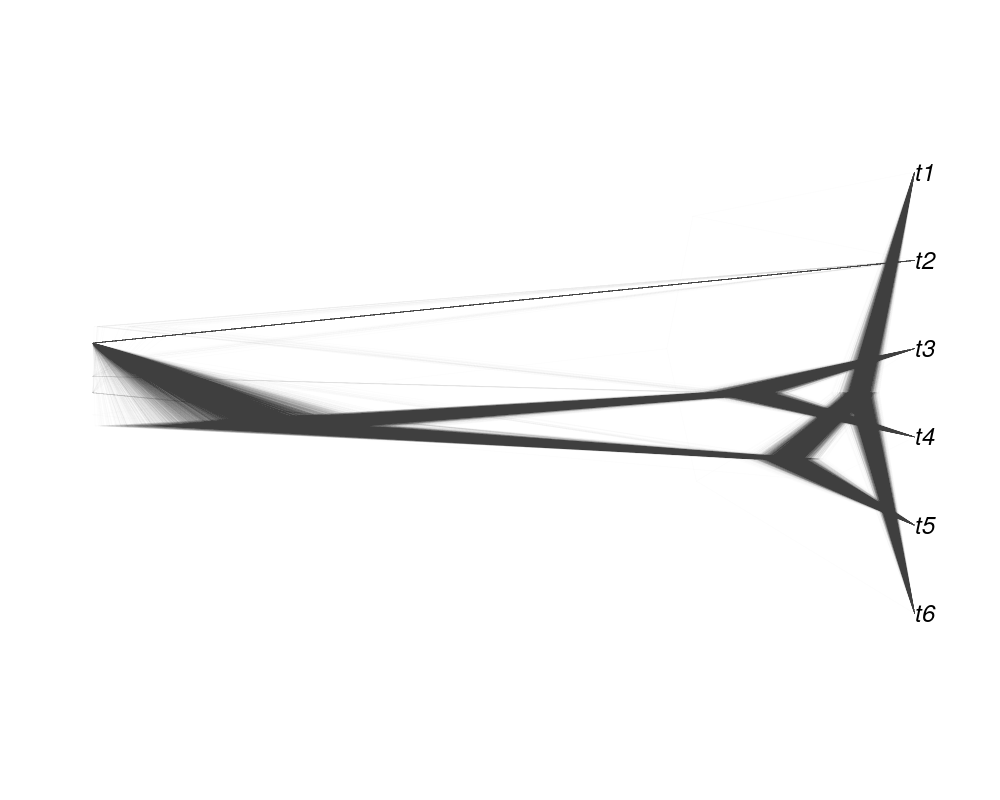
\includegraphics[height=0.45\textheight]{pirouette_example_2/example_2_314/true_posterior_best.png}
    };   
    \node[state] (DB) [right of = DG, rectangle] {
      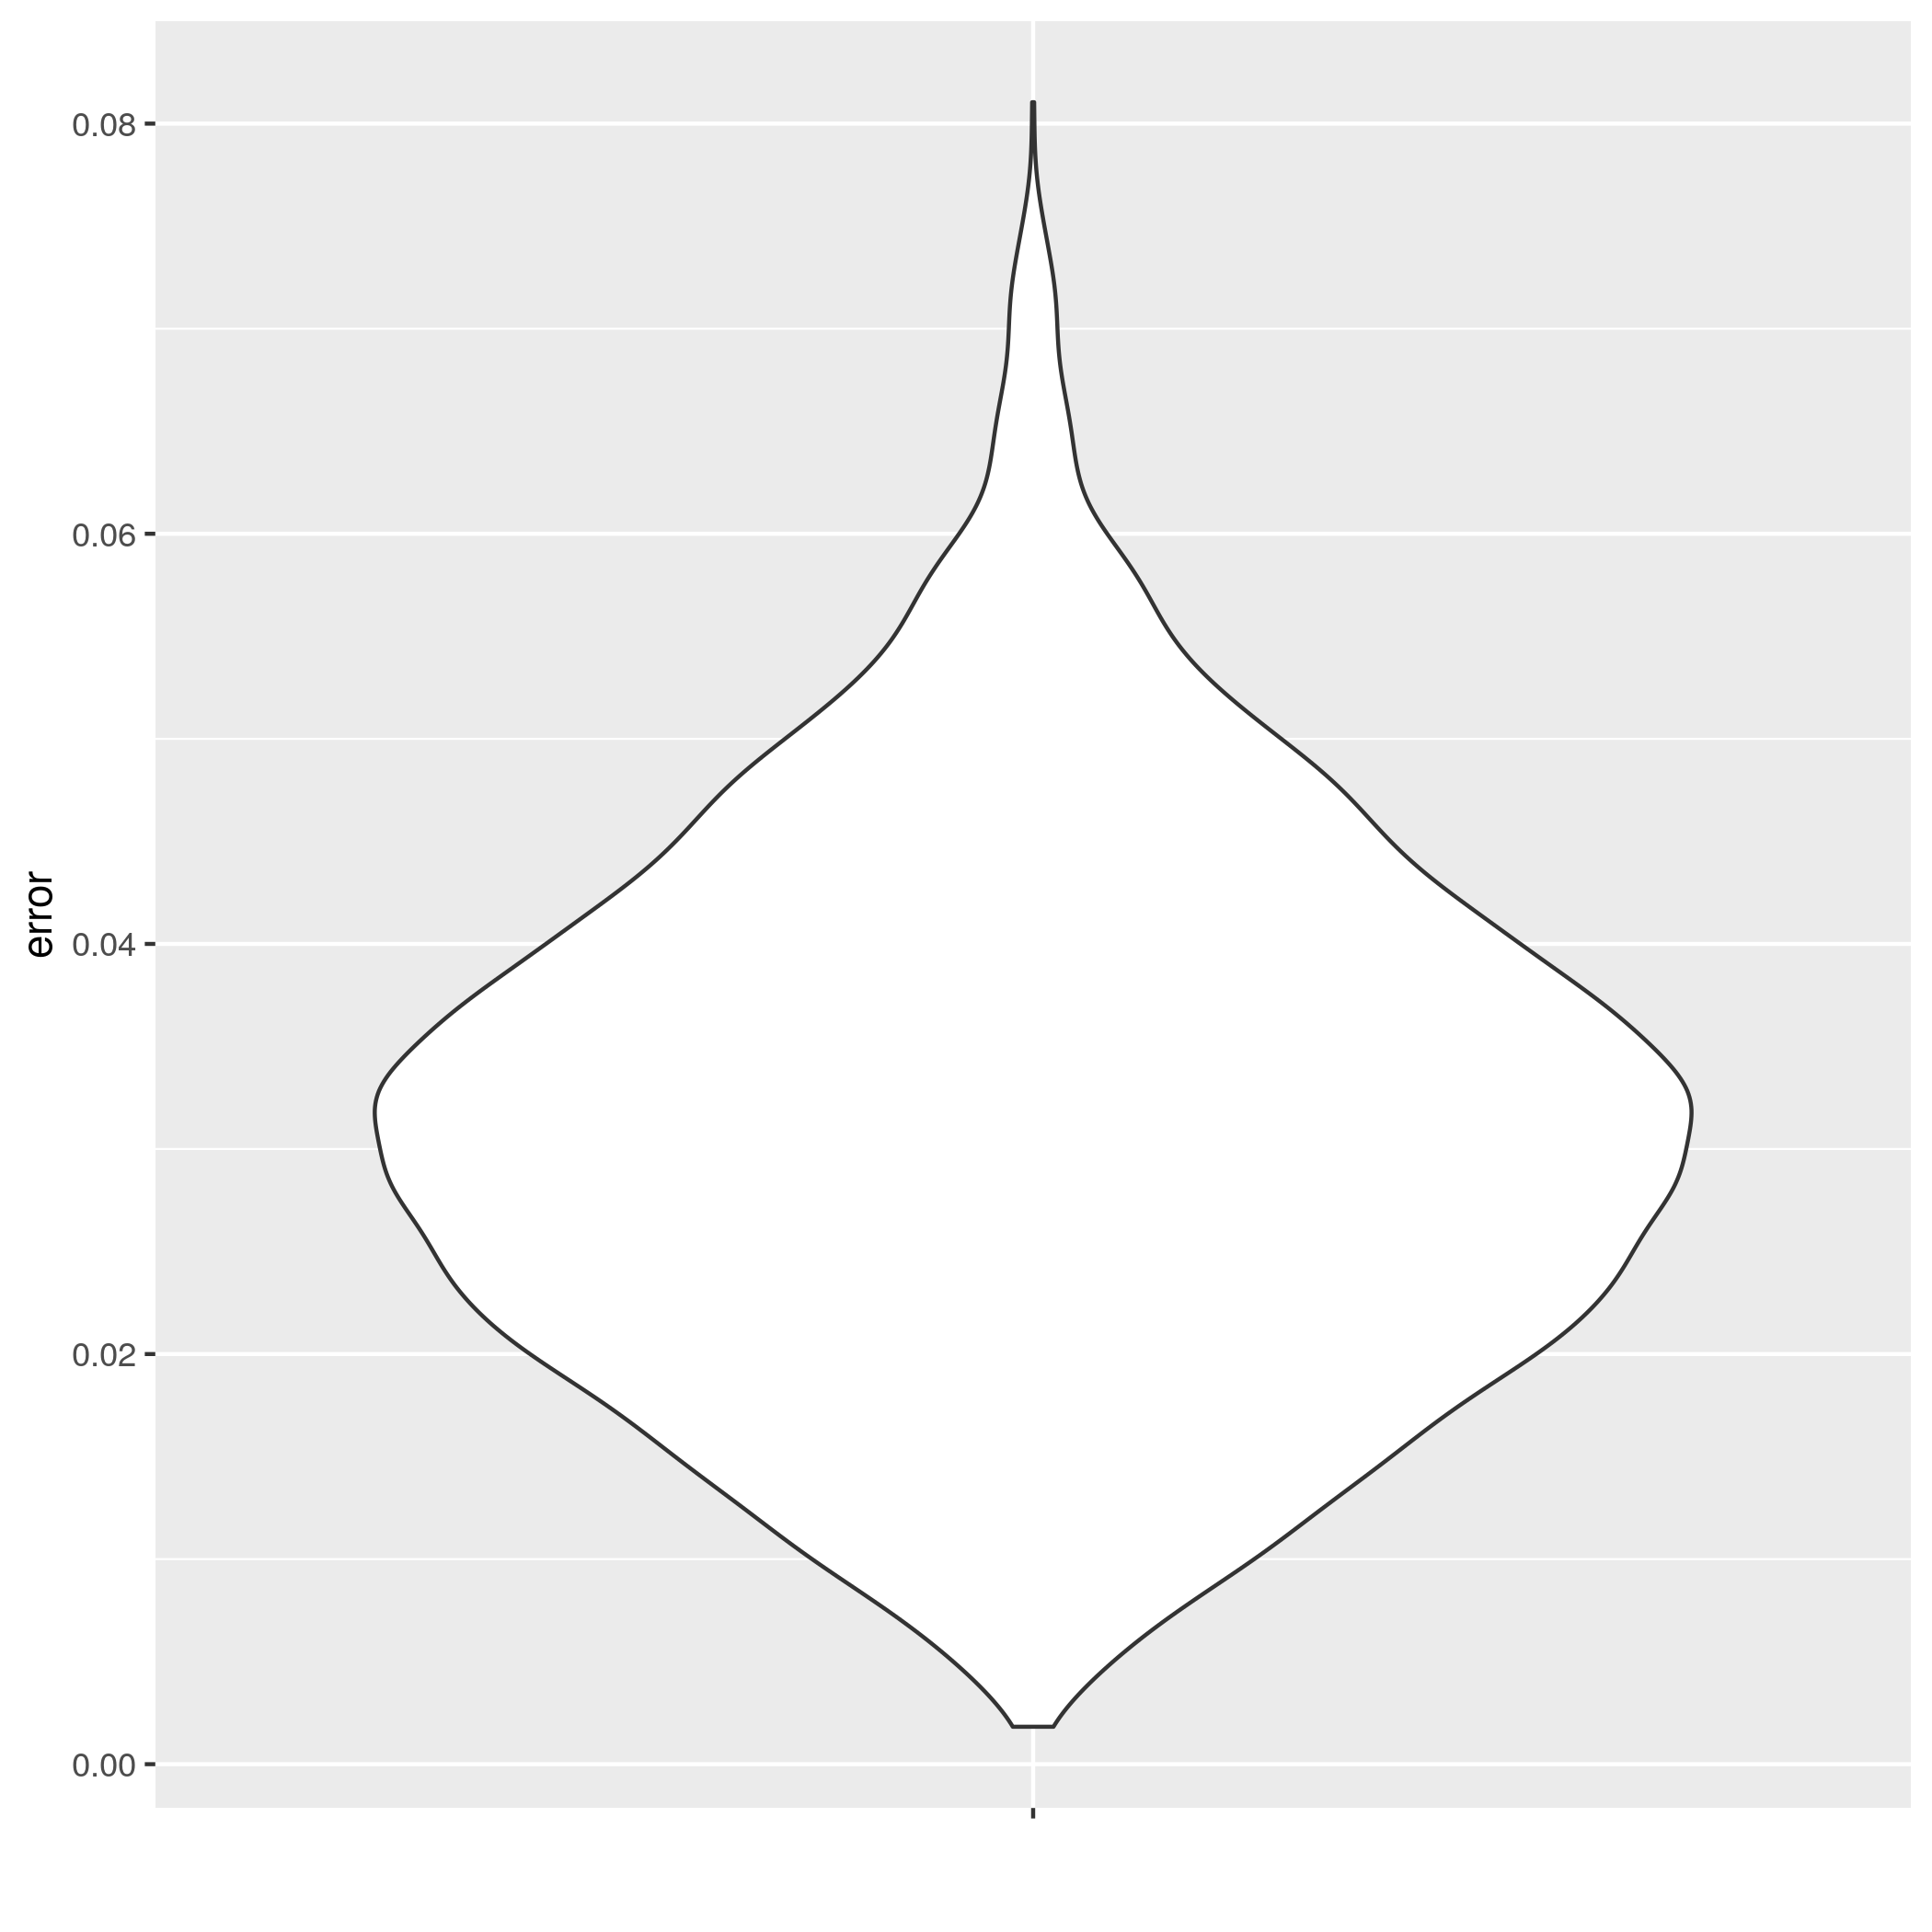
\includegraphics[height=0.3\textheight]{pirouette_example_2/example_2_314/true_error_violin_best.png}
    };   
    \path 
      (O) edge [anchor = south] node {} (A)
      (A) edge [anchor = south] node {} (B)
      (B) edge [anchor = south] node {} (CG)
      (CG) edge [anchor = south] node {} (DG)
      (B) edge [anchor = south] node {} (CB)
      (CB) edge [anchor = south] node {} (DB)
    ; 
    \end{tikzpicture}
  }
  \label{fig:example_2_full_pipeline}
  \caption{Comparing to other candidate models: full pipeline}
\end{figure}
%%%%%%%%%%%%%%%%%%%%%%%%%%%%%%%%%%%%%%%%%%%%%%%%%%%%%%%%%%%%%%%%%%%%%%%%%%%%%%%%

\input{pirouette_example_2/example_2_314/esses_gen.latex}

\input{pirouette_example_2/example_2_314/esses_best.latex}

\input{pirouette_example_2/example_2_314/evidence_true.latex}

%%%%%%%%%%%%%%%%%%%%%%%%%%%%%%%%%%%%%%%%%%%%%%%%%%%%%%%%%%%%%%%%%%%%%%%%%%%%%%%%
\subsection{Comparing to background noise}
%%%%%%%%%%%%%%%%%%%%%%%%%%%%%%%%%%%%%%%%%%%%%%%%%%%%%%%%%%%%%%%%%%%%%%%%%%%%%%%%

The code used in this part of the article can be found at 
\url{https://github.com/richelbilderbeek/pirouette_example_3}.

%%%%%%%%%%%%%%%%%%%%%%%%%%%%%%%%%%%%%%%%%%%%%%%%%%%%%%%%%%%%%%%%%%%%%%%%%%%%%%%%
\begin{figure}[H]
  \centering
  \resizebox {1.0\columnwidth} {!} {
    \begin{tikzpicture}[
      ->,>=stealth',shorten >=1pt,auto,
      node distance=0.5\textheight, 
      semithick
    ]   
    \tikzstyle{every state}=[]
    \node[state, draw=none] (O) [] {
    };   
    \node[state] (A) [right of = O, rectangle] {
      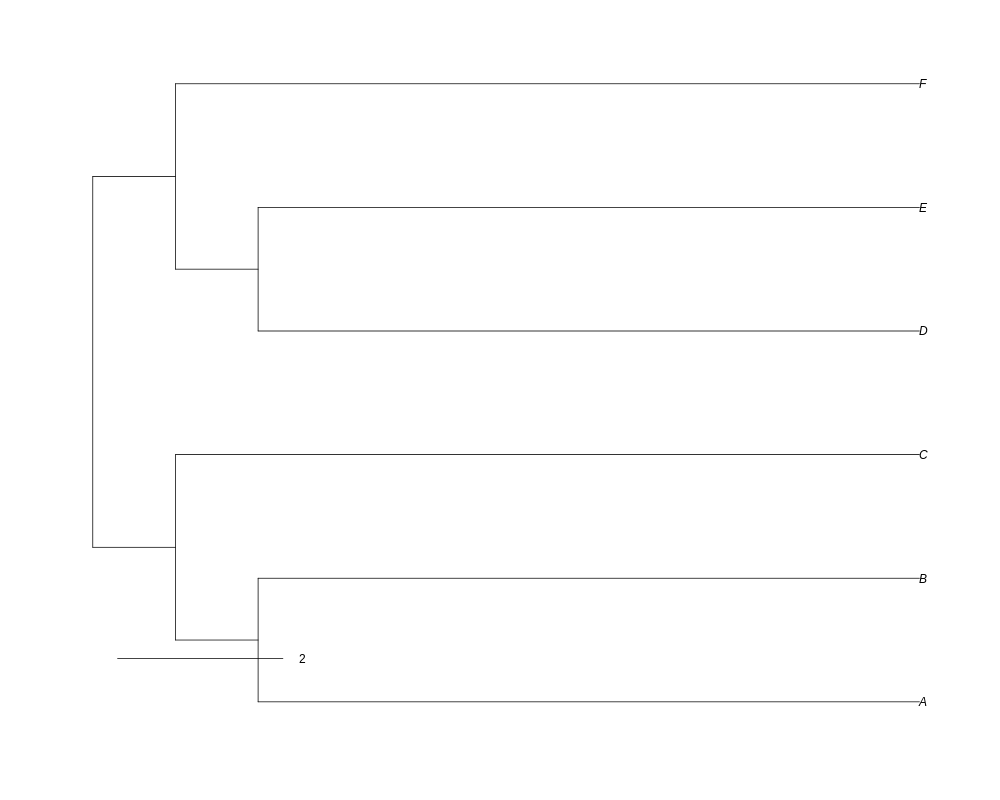
\includegraphics[height=0.4\textheight]{pirouette_example_3/example_3_314/true_tree.png}
    };   
    \node[state] (B) [below of = A, rectangle] {
      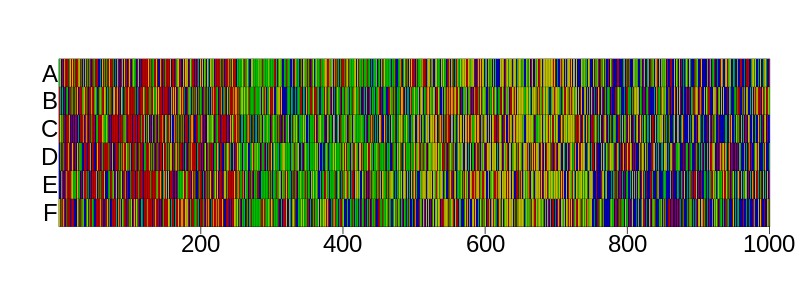
\includegraphics[height=0.25\textheight]{pirouette_example_3/example_3_314/true_alignment.png}
    };   
    \node[state] (CG) [below of = B, rectangle] {
      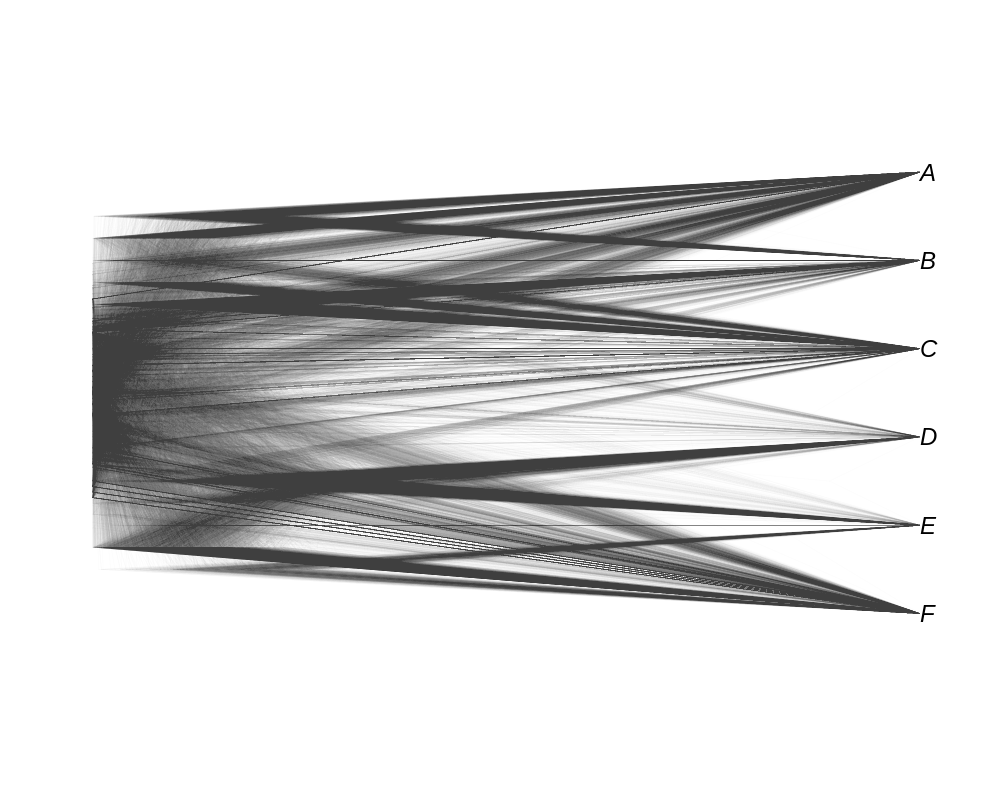
\includegraphics[height=0.3\textheight]{pirouette_example_3/example_3_314/true_posterior_gen.png}
    };   
    \node[state] (DG) [below of = CG, rectangle] {
      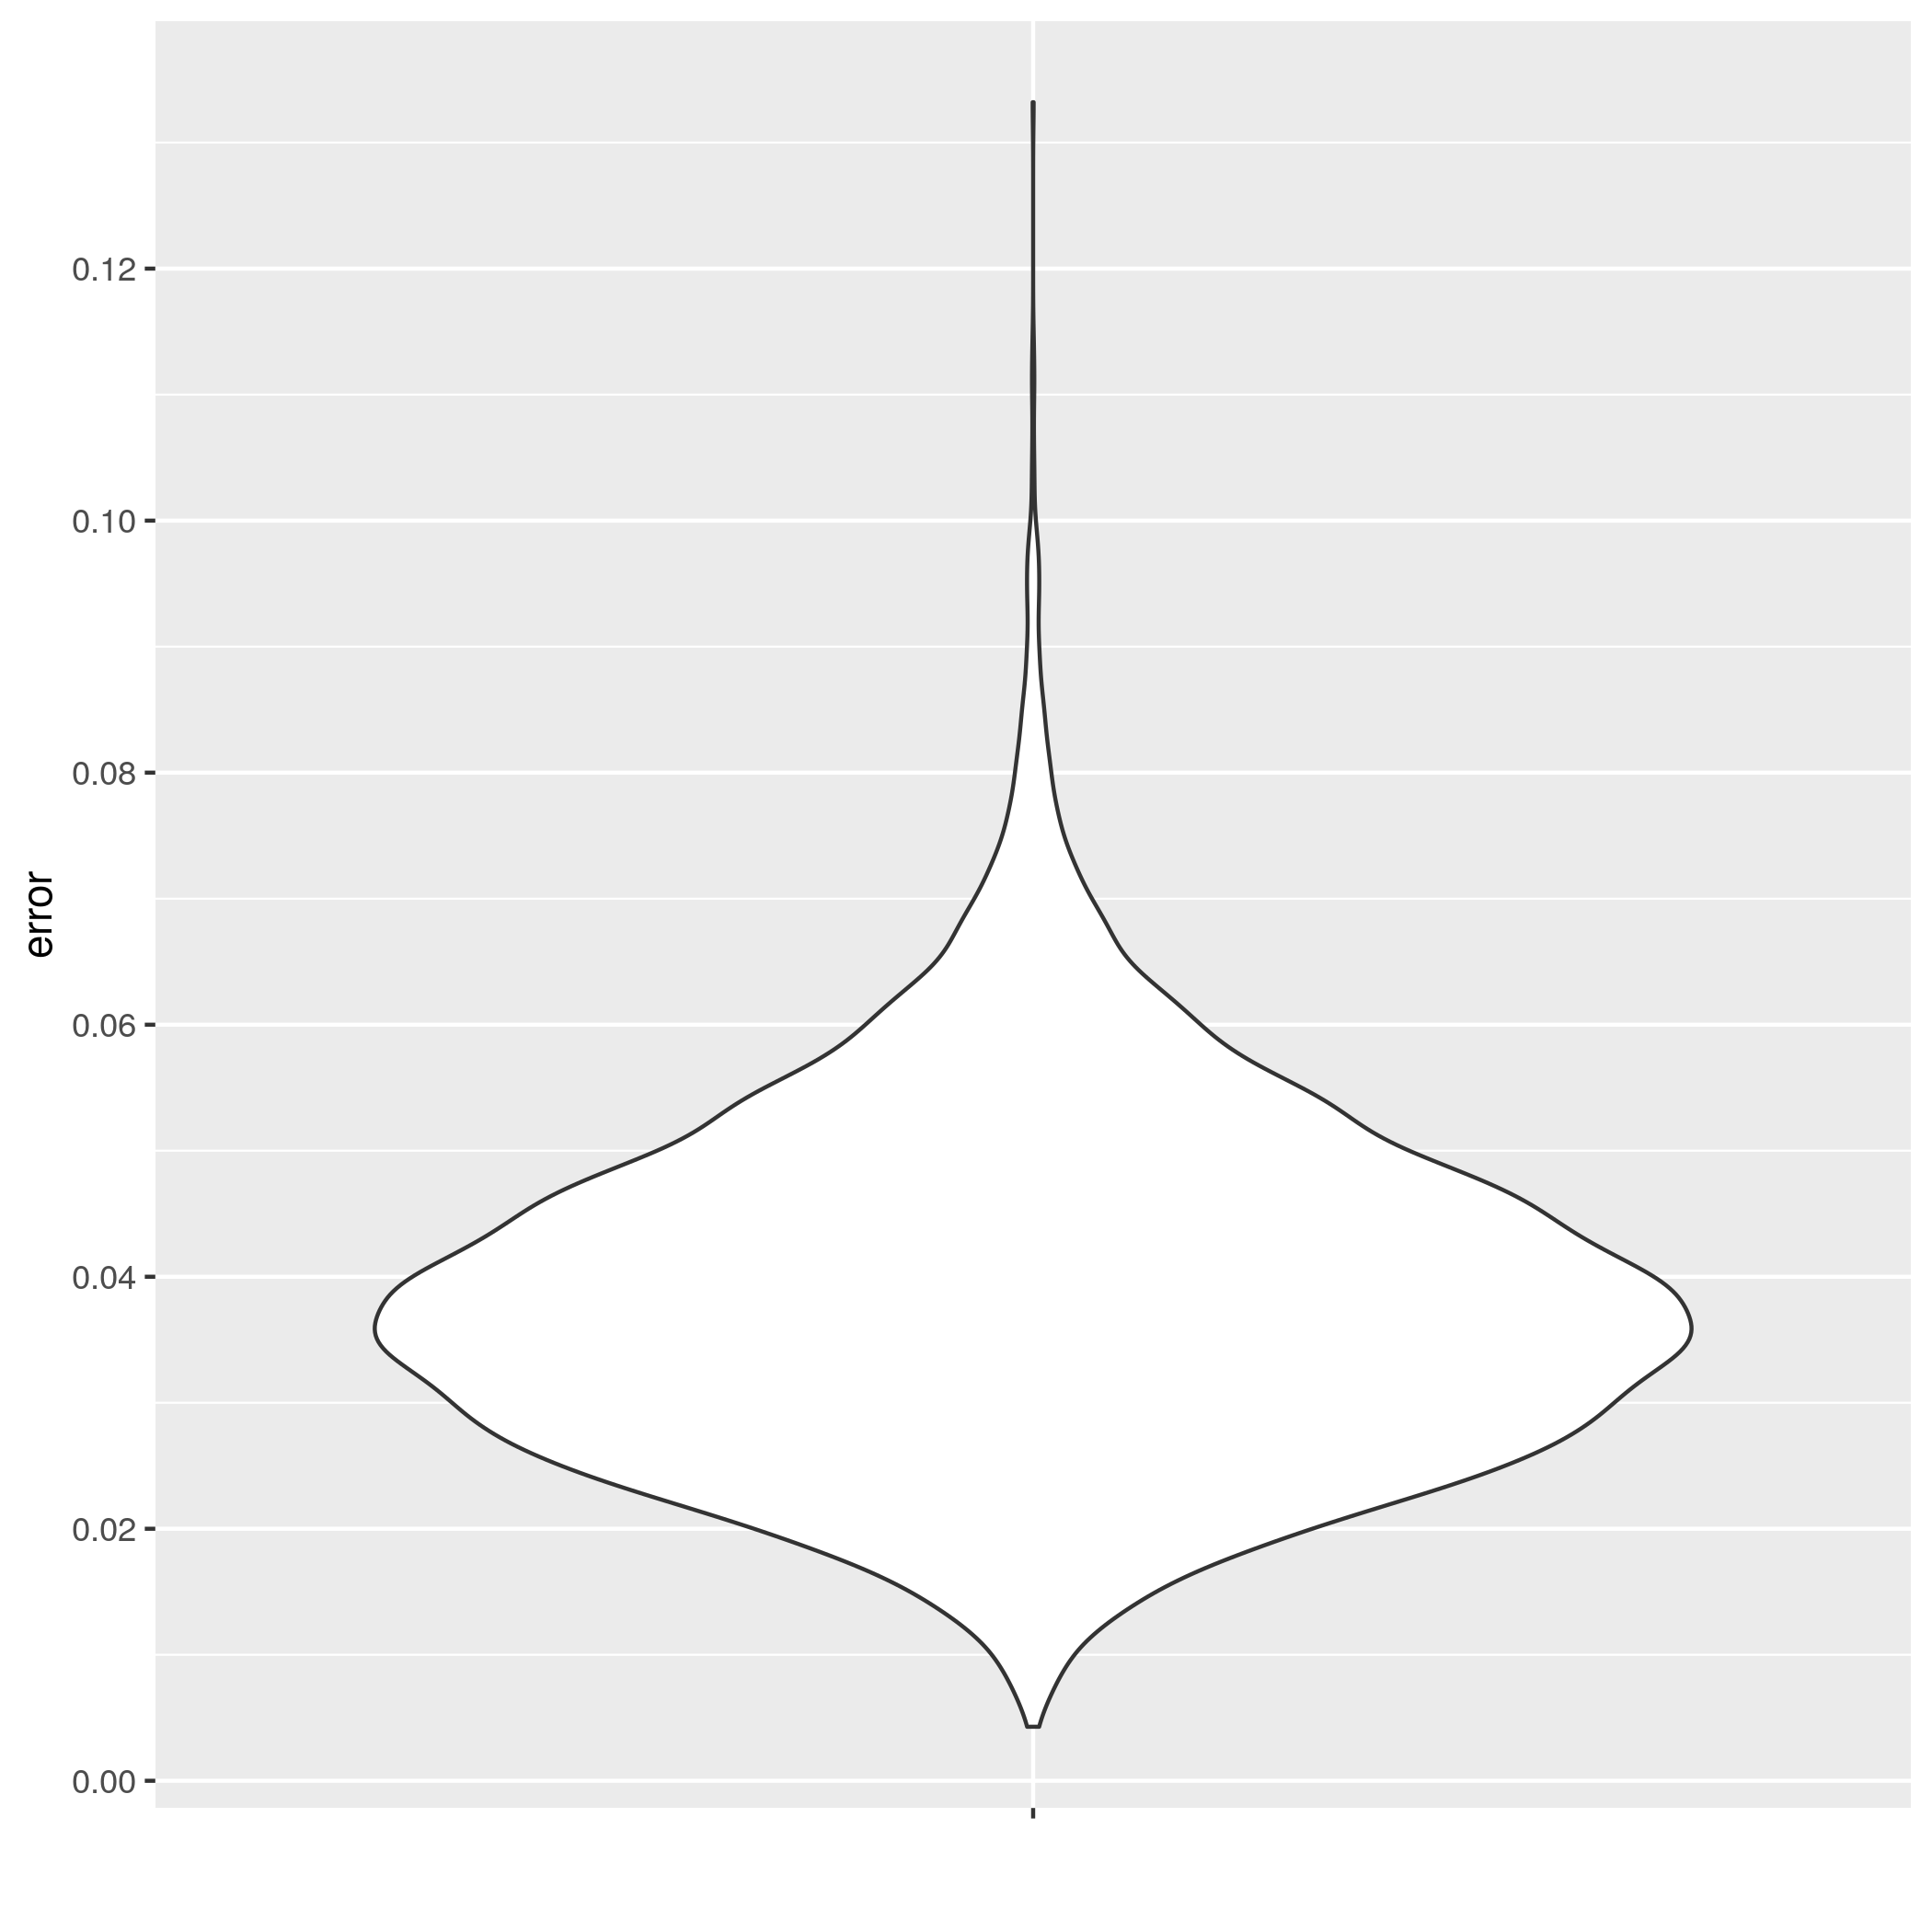
\includegraphics[height=0.3\textheight]{pirouette_example_3/example_3_314/true_error_violin_gen.png}
    };   
    \node[state] (CB) [right of = CG, rectangle] {
      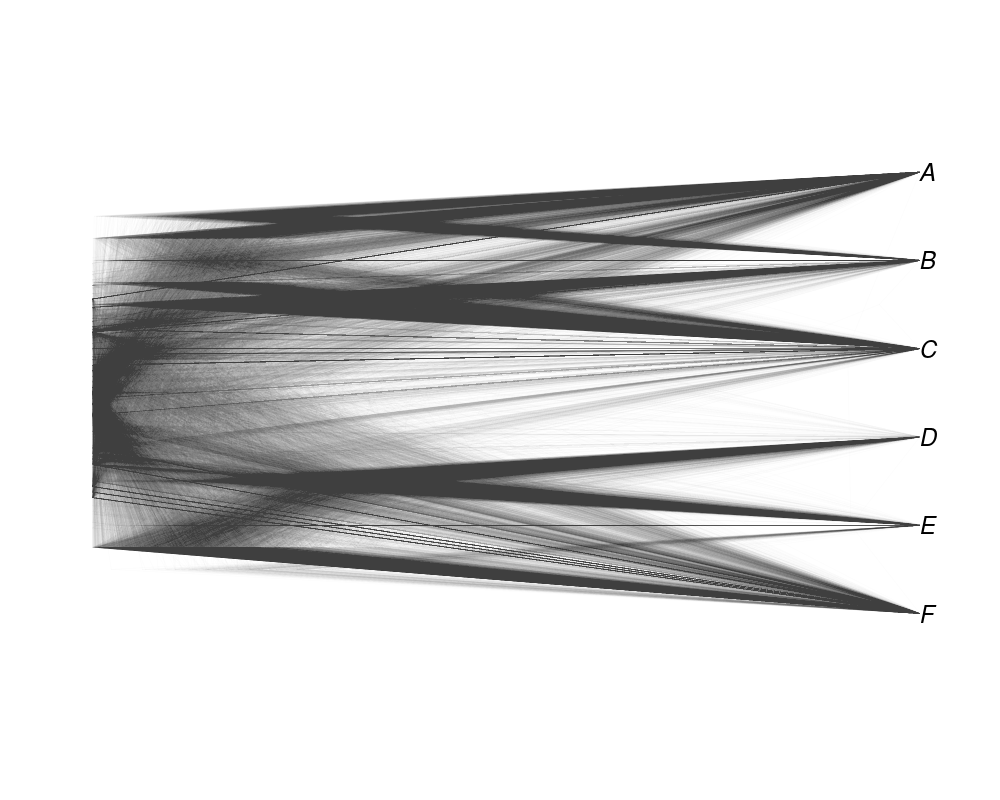
\includegraphics[height=0.3\textheight]{pirouette_example_3/example_3_314/true_posterior_best.png}
    };   
    \node[state] (DB) [below of = CB, rectangle] {
      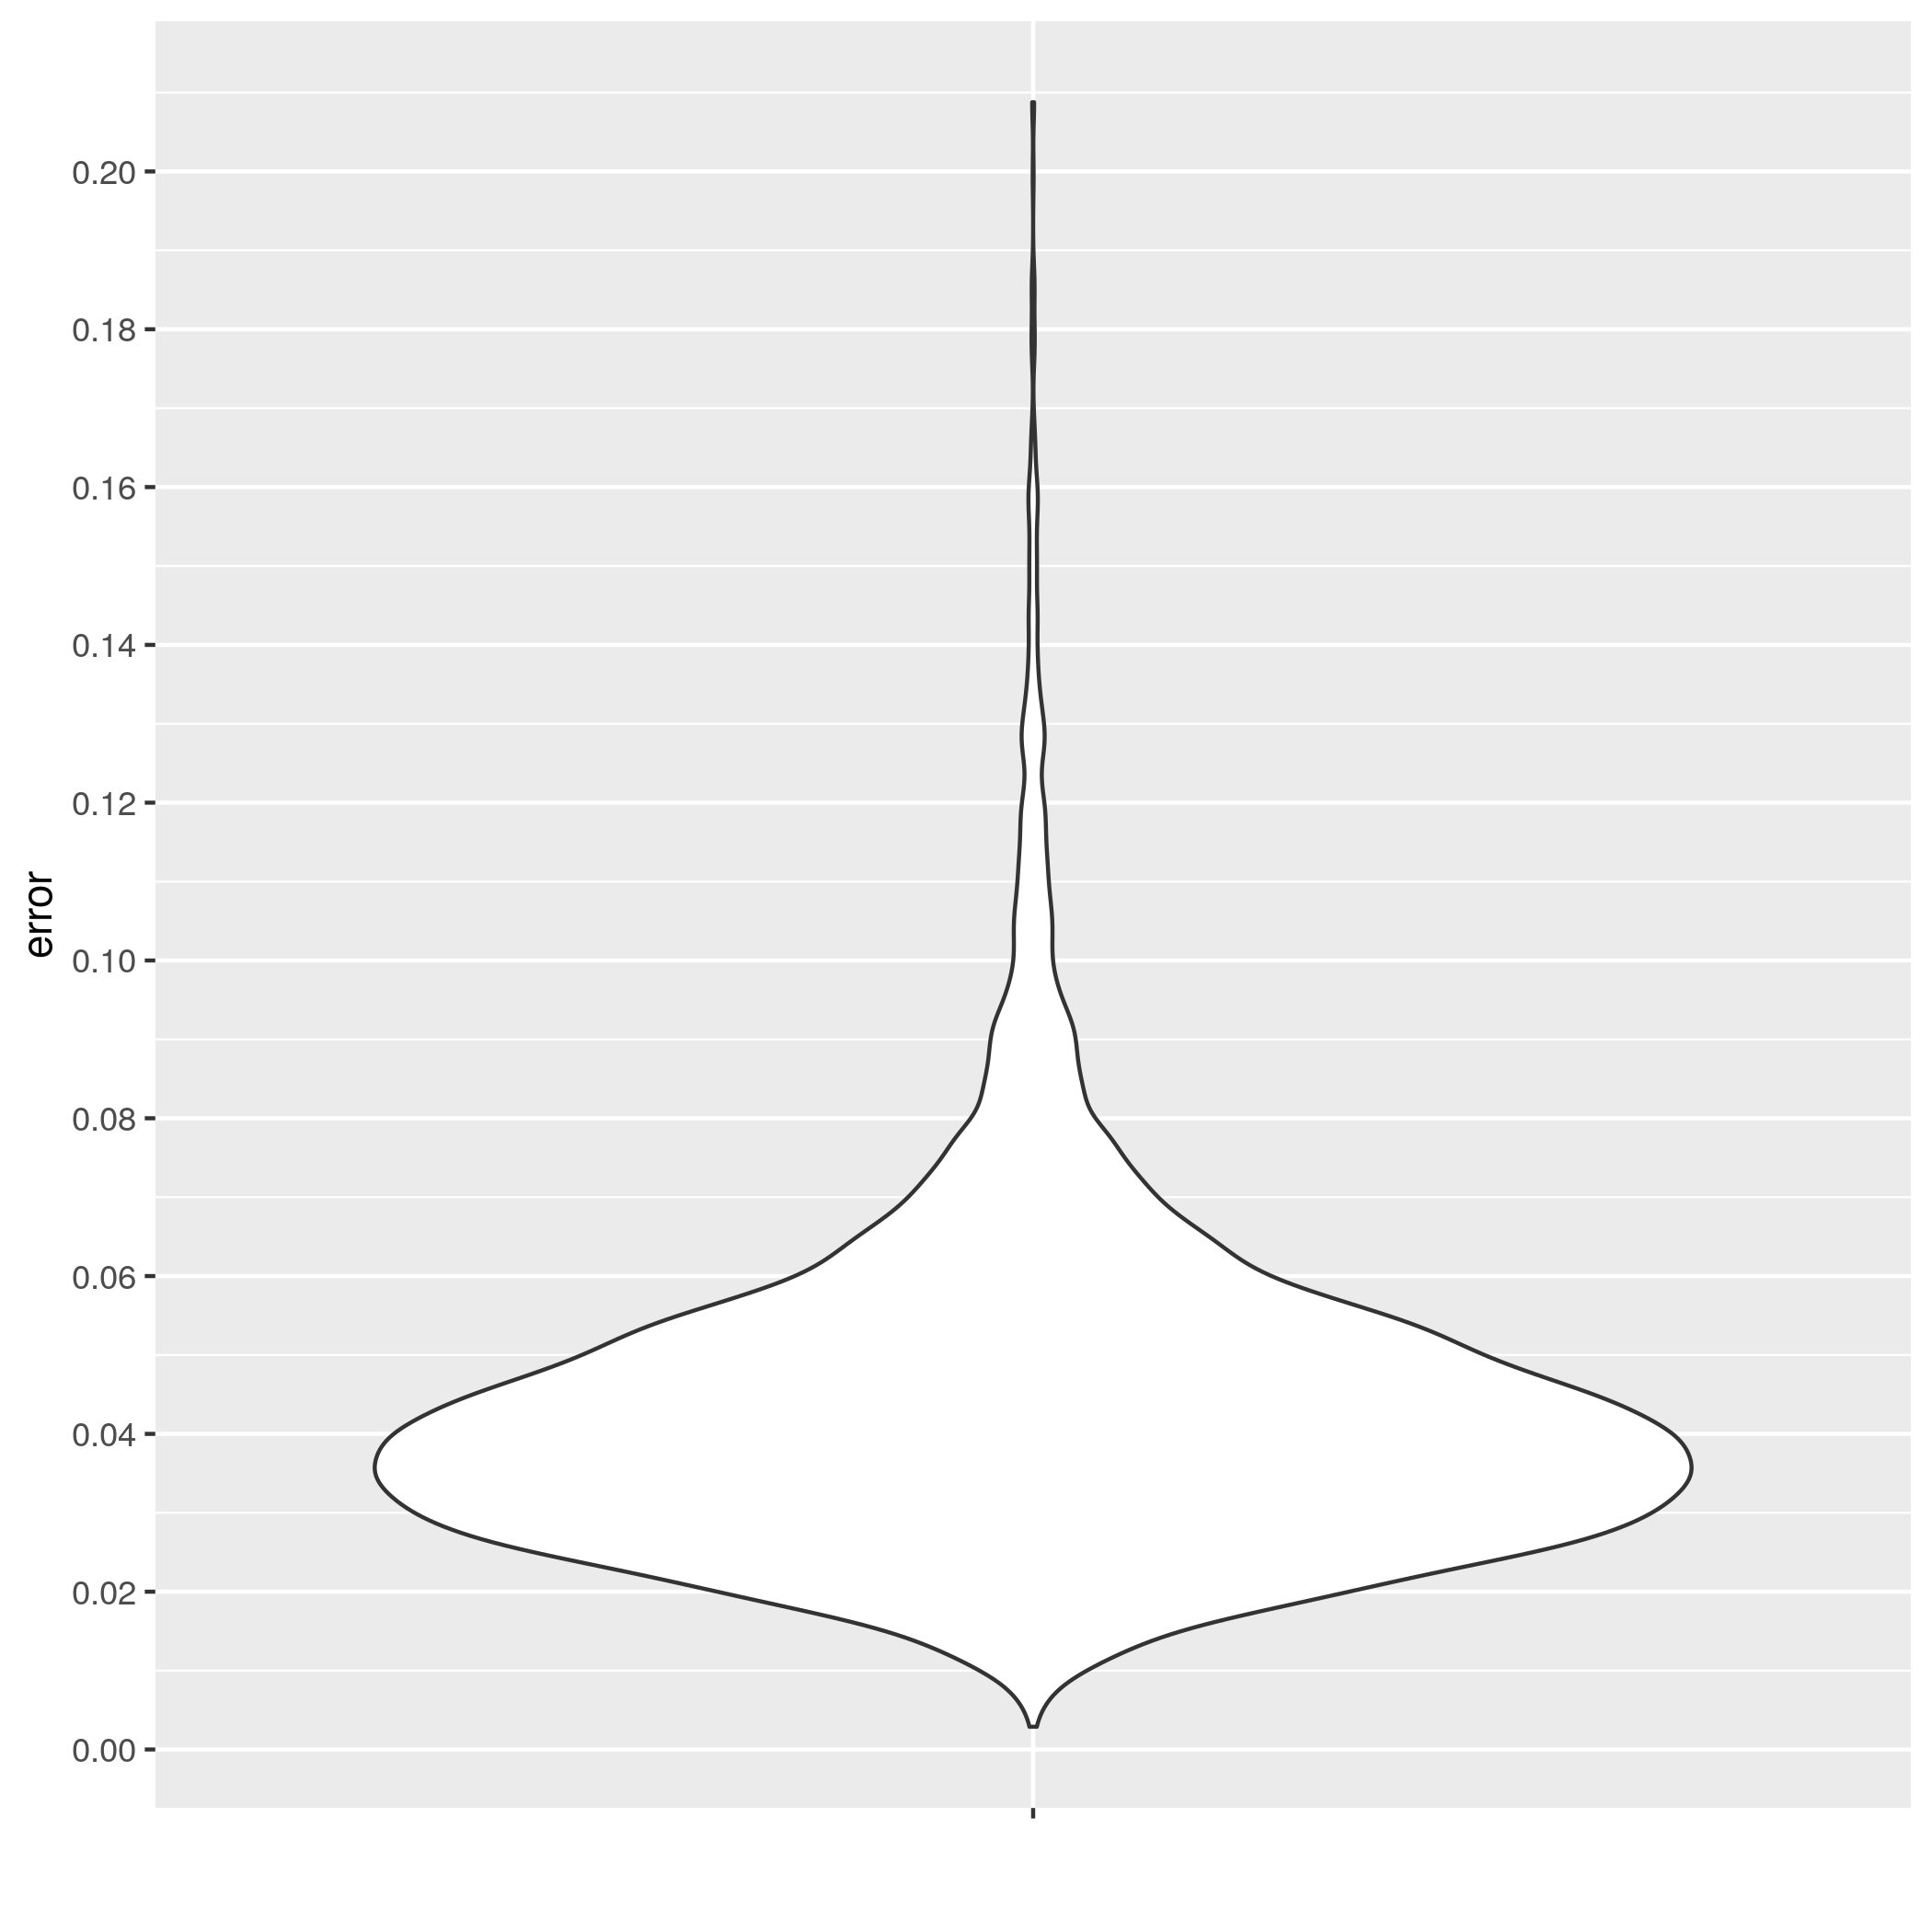
\includegraphics[height=0.3\textheight]{pirouette_example_3/example_3_314/true_error_violin_best.png}
    };   
    \node[state] (AT) [right of = A, rectangle, node distance=0.8\textheight] {
      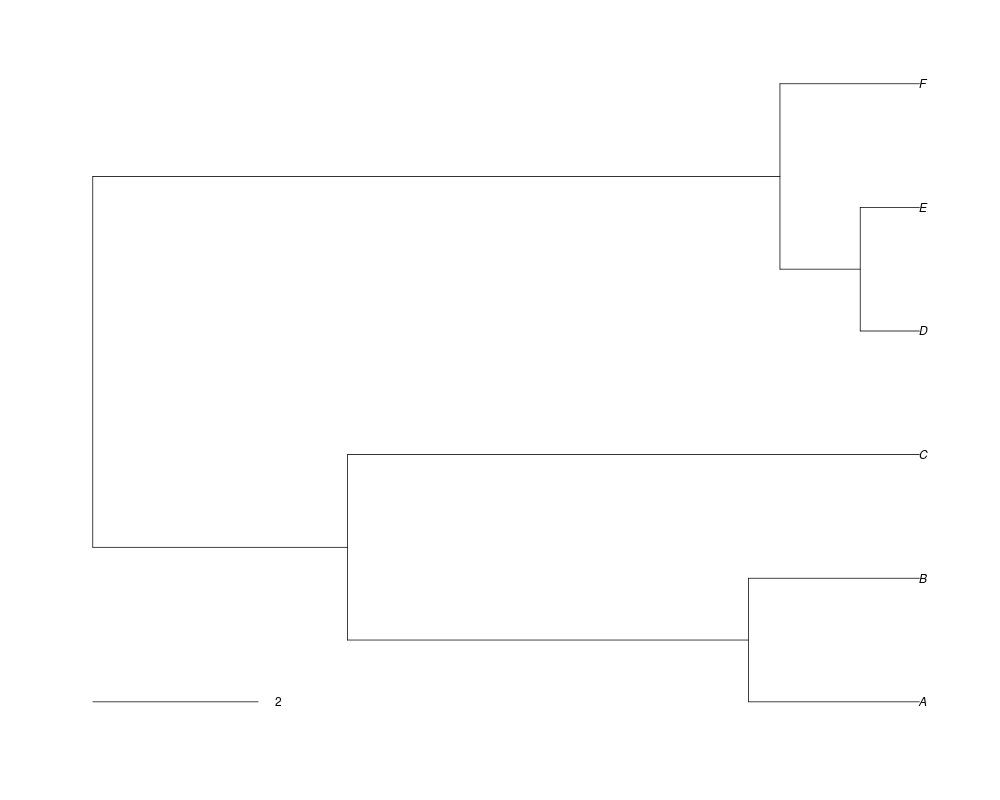
\includegraphics[height=0.4\textheight]{pirouette_example_3/example_3_314/twin_tree.png}
    };   
    \node[state] (BT) [below of = AT, rectangle] {
      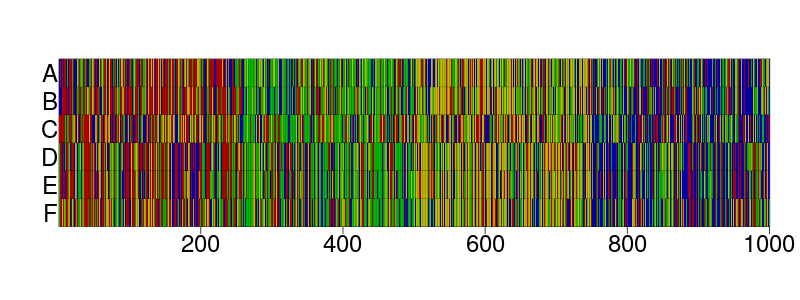
\includegraphics[height=0.25\textheight]{pirouette_example_3/example_3_314/twin_alignment.png}
    };   
    \node[state] (CTG) [right of = CB, rectangle] {
      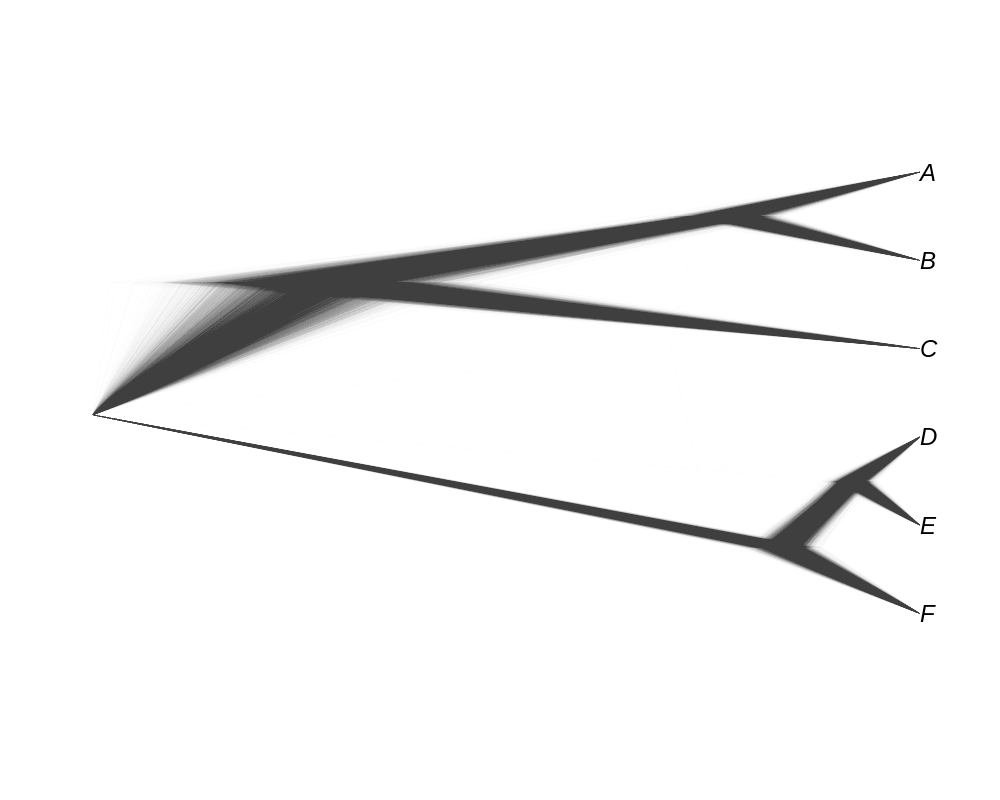
\includegraphics[height=0.3\textheight]{pirouette_example_3/example_3_314/twin_posterior_gen.png}
    };   
    \node[state] (DTG) [below of = CTG, rectangle] {
      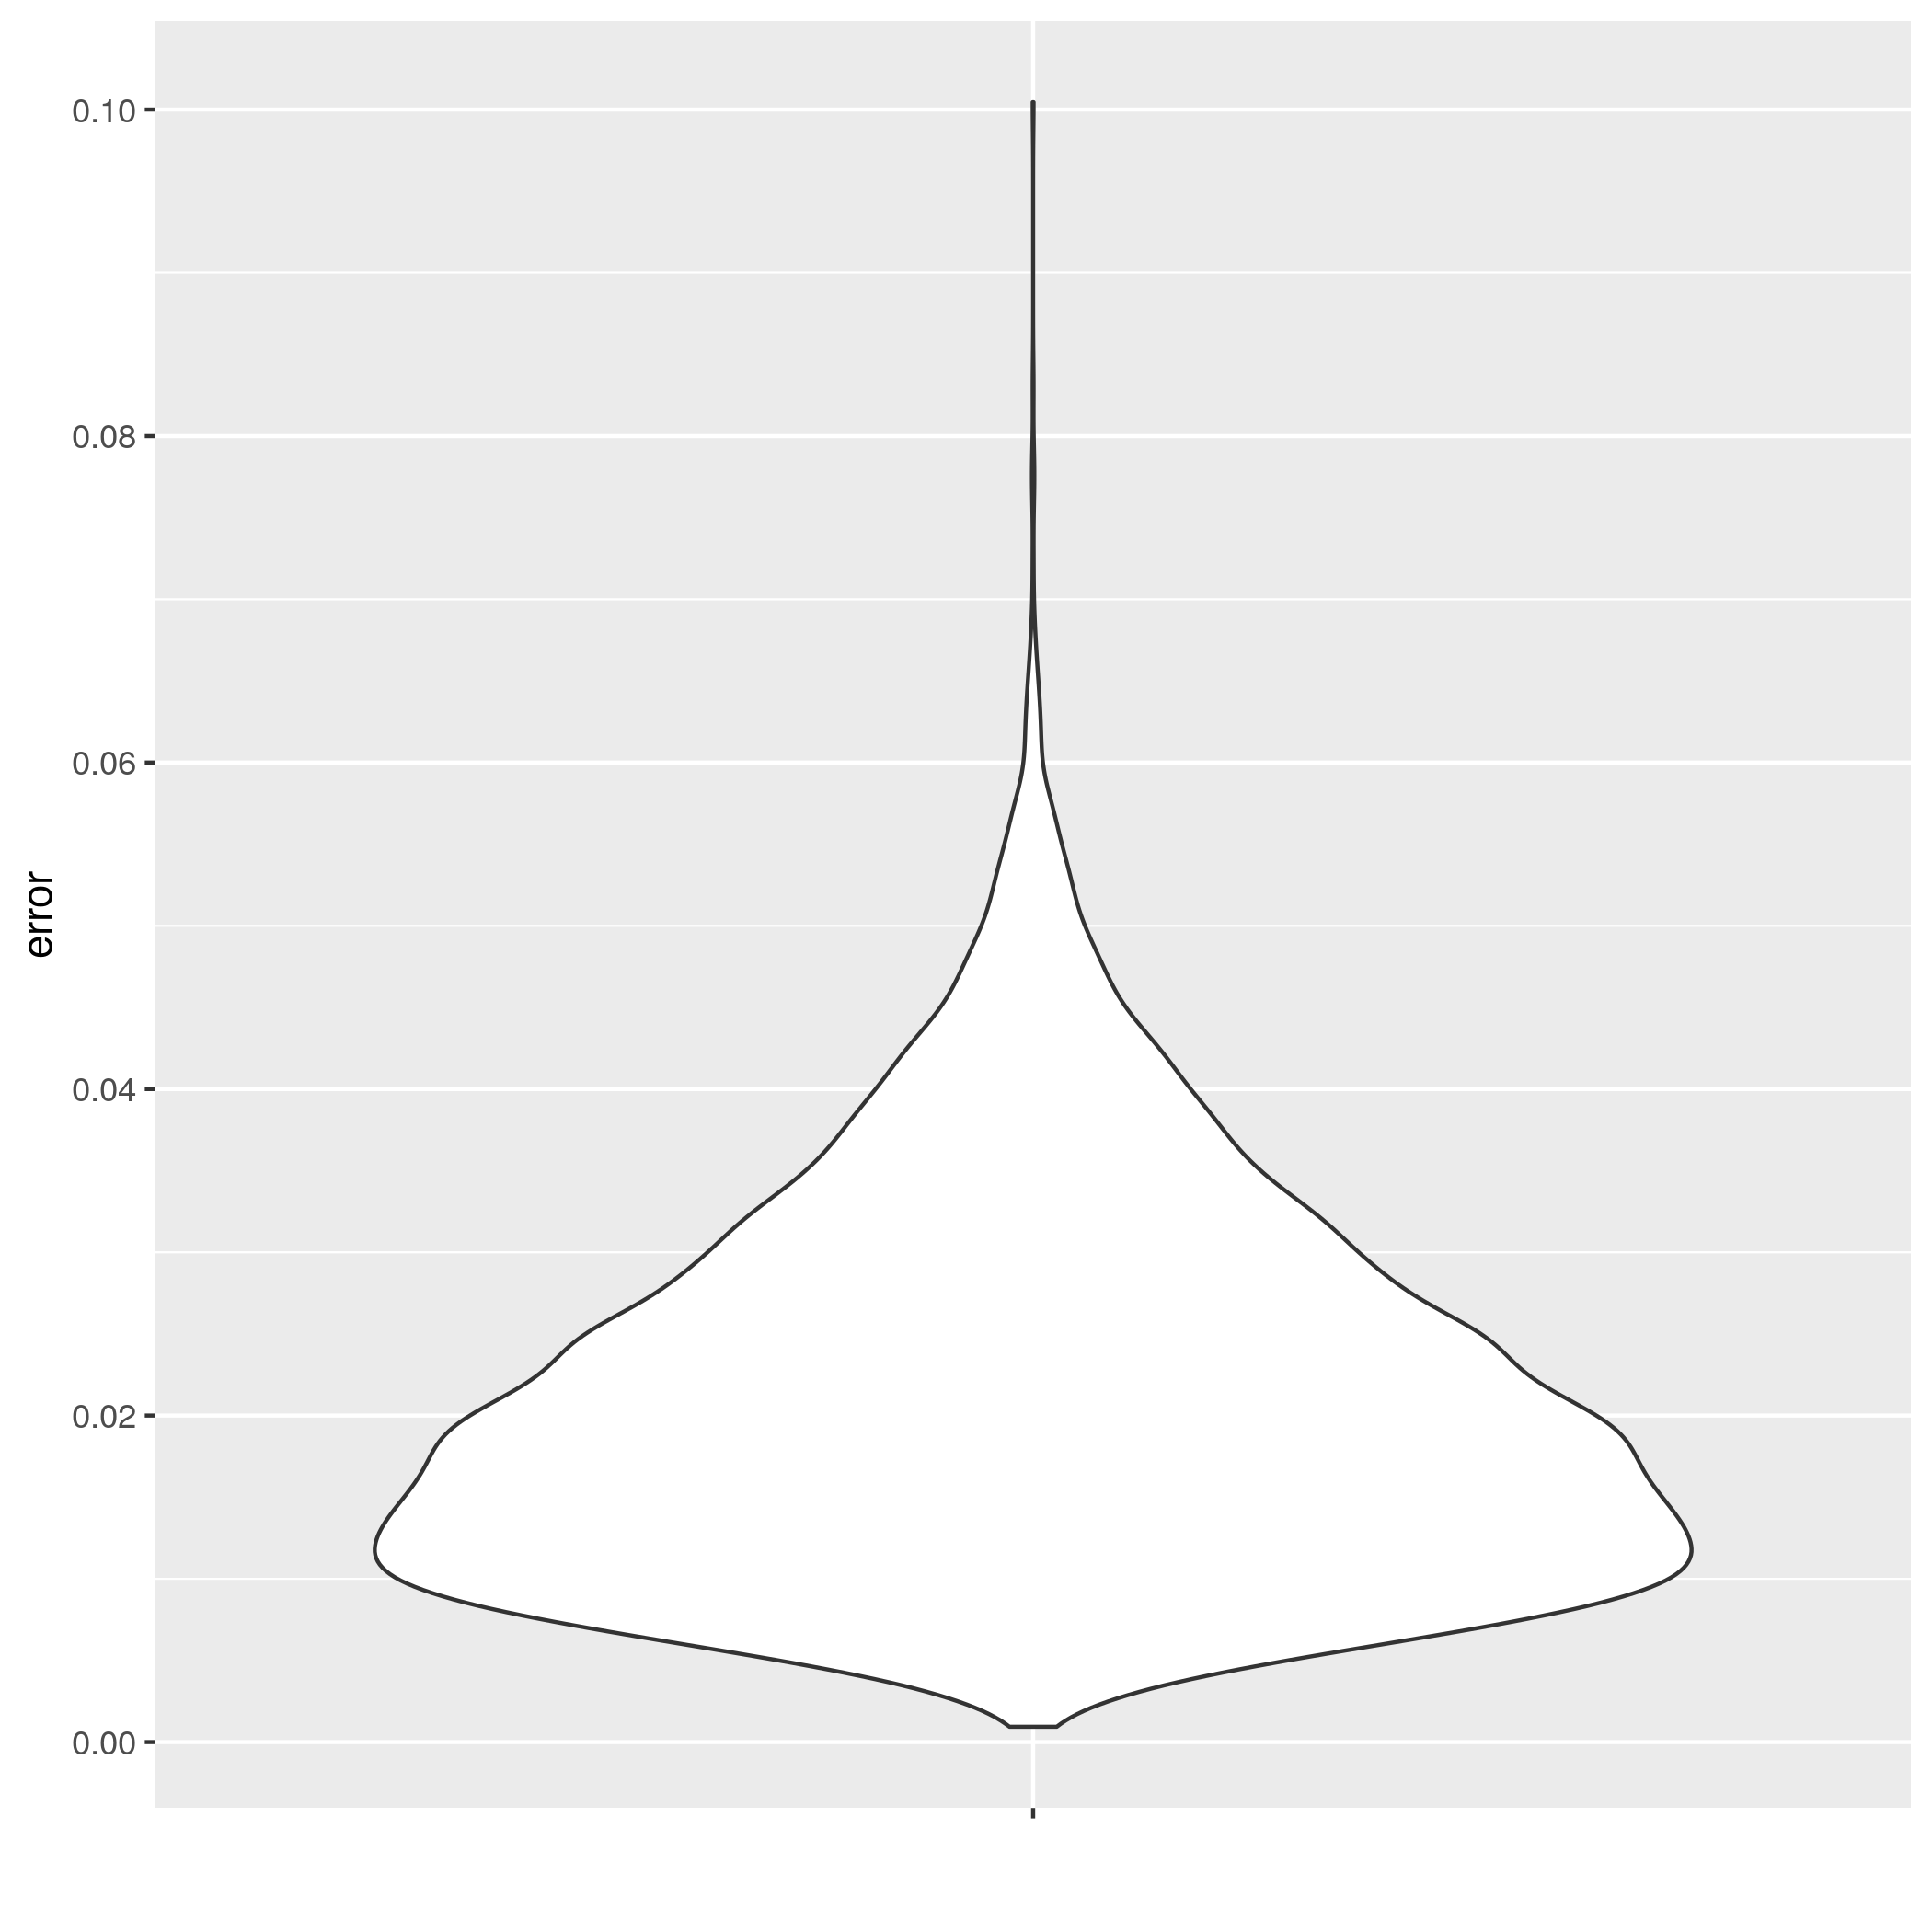
\includegraphics[height=0.3\textheight]{pirouette_example_3/example_3_314/twin_error_violin_gen.png}
    };   
    \node[state] (CTB) [right of = CTG, rectangle] {
      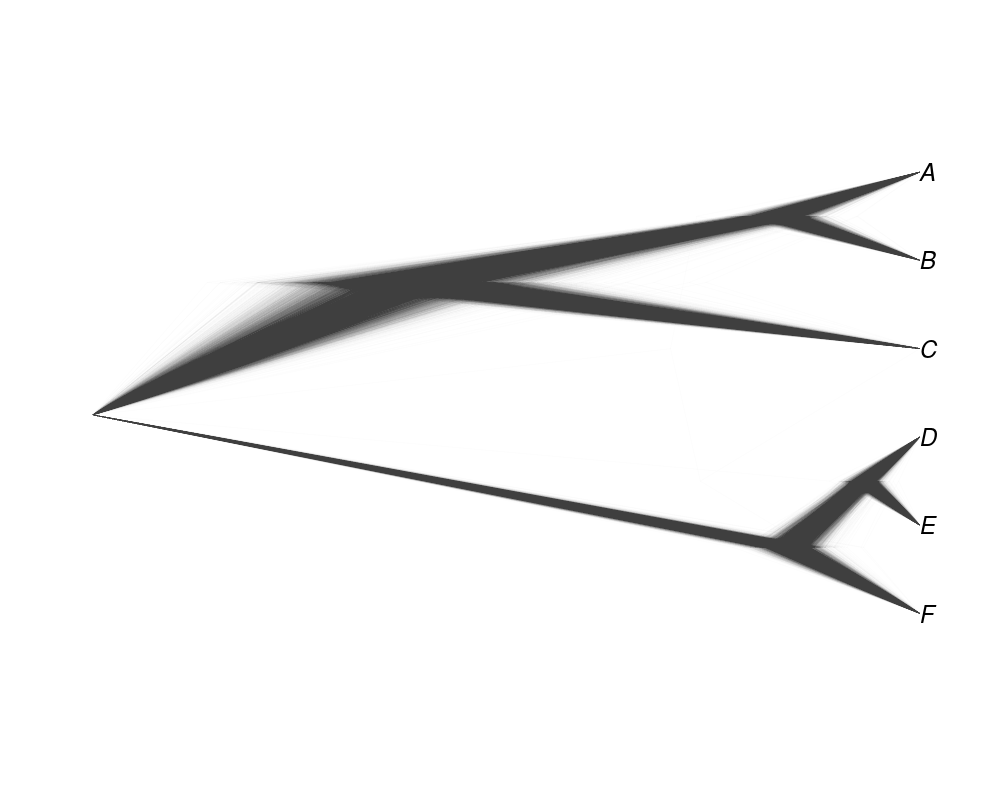
\includegraphics[height=0.3\textheight]{pirouette_example_3/example_3_314/twin_posterior_best.png}
    };   
    \node[state] (DTB) [below of = CTB, rectangle] {
      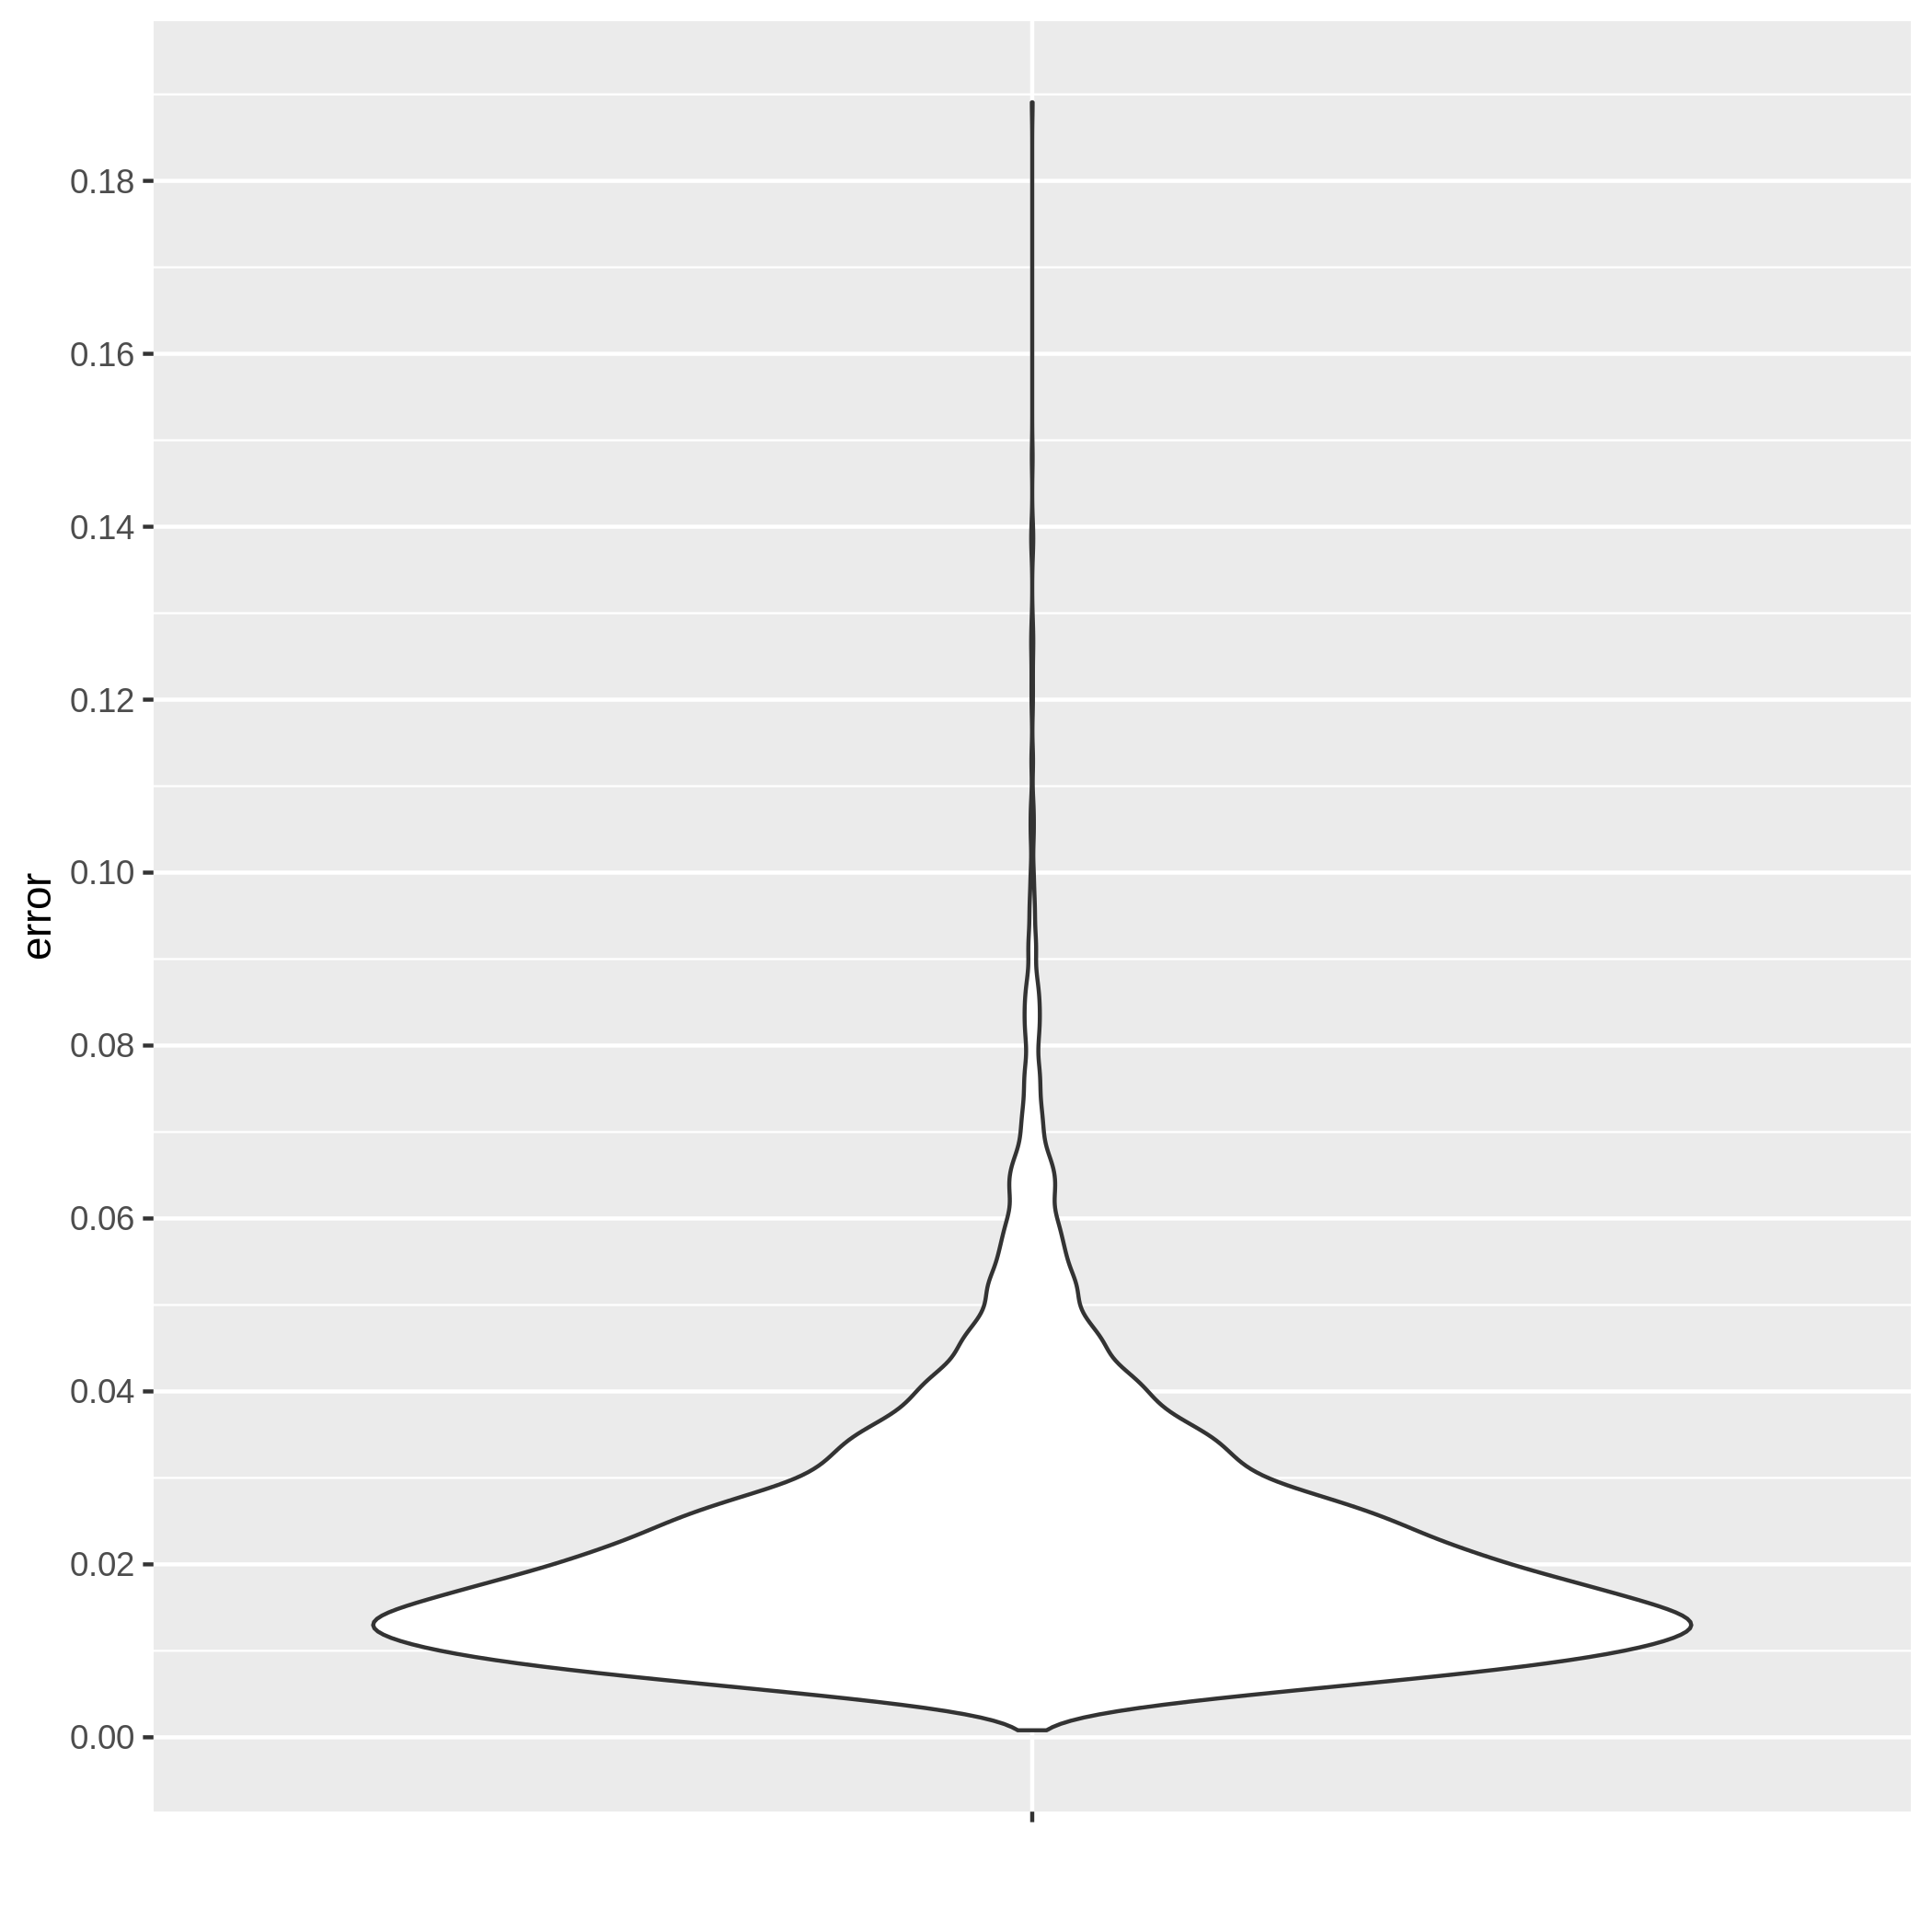
\includegraphics[height=0.3\textheight]{pirouette_example_3/example_3_314/twin_error_violin_best.png}
    };   
    \path 
      (O) edge [anchor = south] node {} (A)
      (A) edge [anchor = south] node {} (B)
      (B) edge [anchor = south] node {} (CG)
      (CG) edge [anchor = south] node {} (DG)
      (B) edge [anchor = south east] node {} (CB)
      (CB) edge [anchor = south] node {} (DB)
      (A) edge [anchor = east] node {} (AT)
      (AT) edge [anchor = south] node {} (BT)
      (BT) edge [anchor = south east] node {} (CTG)
      (CTG) edge [anchor = south] node {} (DTG)
      (BT) edge [anchor = south] node {} (CTB)
      (CTB) edge [anchor = south] node {} (DTB)
    ; 
    \end{tikzpicture}
  }
  \label{fig:example_3_full_pipeline}
  \caption{Comparing to background noise: full pipeline}
\end{figure}
%%%%%%%%%%%%%%%%%%%%%%%%%%%%%%%%%%%%%%%%%%%%%%%%%%%%%%%%%%%%%%%%%%%%%%%%%%%%%%%%

\input{pirouette_example_3/example_3_314/esses_gen.latex}

\input{pirouette_example_3/example_3_314/esses_best.latex}

\input{pirouette_example_3/example_3_314/esses_twin_gen.latex}

\input{pirouette_example_3/example_3_314/esses_twin_best.latex}

\input{pirouette_example_3/example_3_314/evidence_true.latex}

\input{pirouette_example_3/example_3_314/evidence_twin.latex}

%%%%%%%%%%%%%%%%%%%%%%%%%%%%%%%%%%%%%%%%%%%%%%%%%%%%%%%%%%%%%%%%%%%%%%%%%%%%%%%%
\subsection{The effect of the number of taxa}
%%%%%%%%%%%%%%%%%%%%%%%%%%%%%%%%%%%%%%%%%%%%%%%%%%%%%%%%%%%%%%%%%%%%%%%%%%%%%%%%

The code used in this part of the article can be found at 
\url{https://github.com/richelbilderbeek/pirouette_example_20}. 

\begin{figure}[H]
  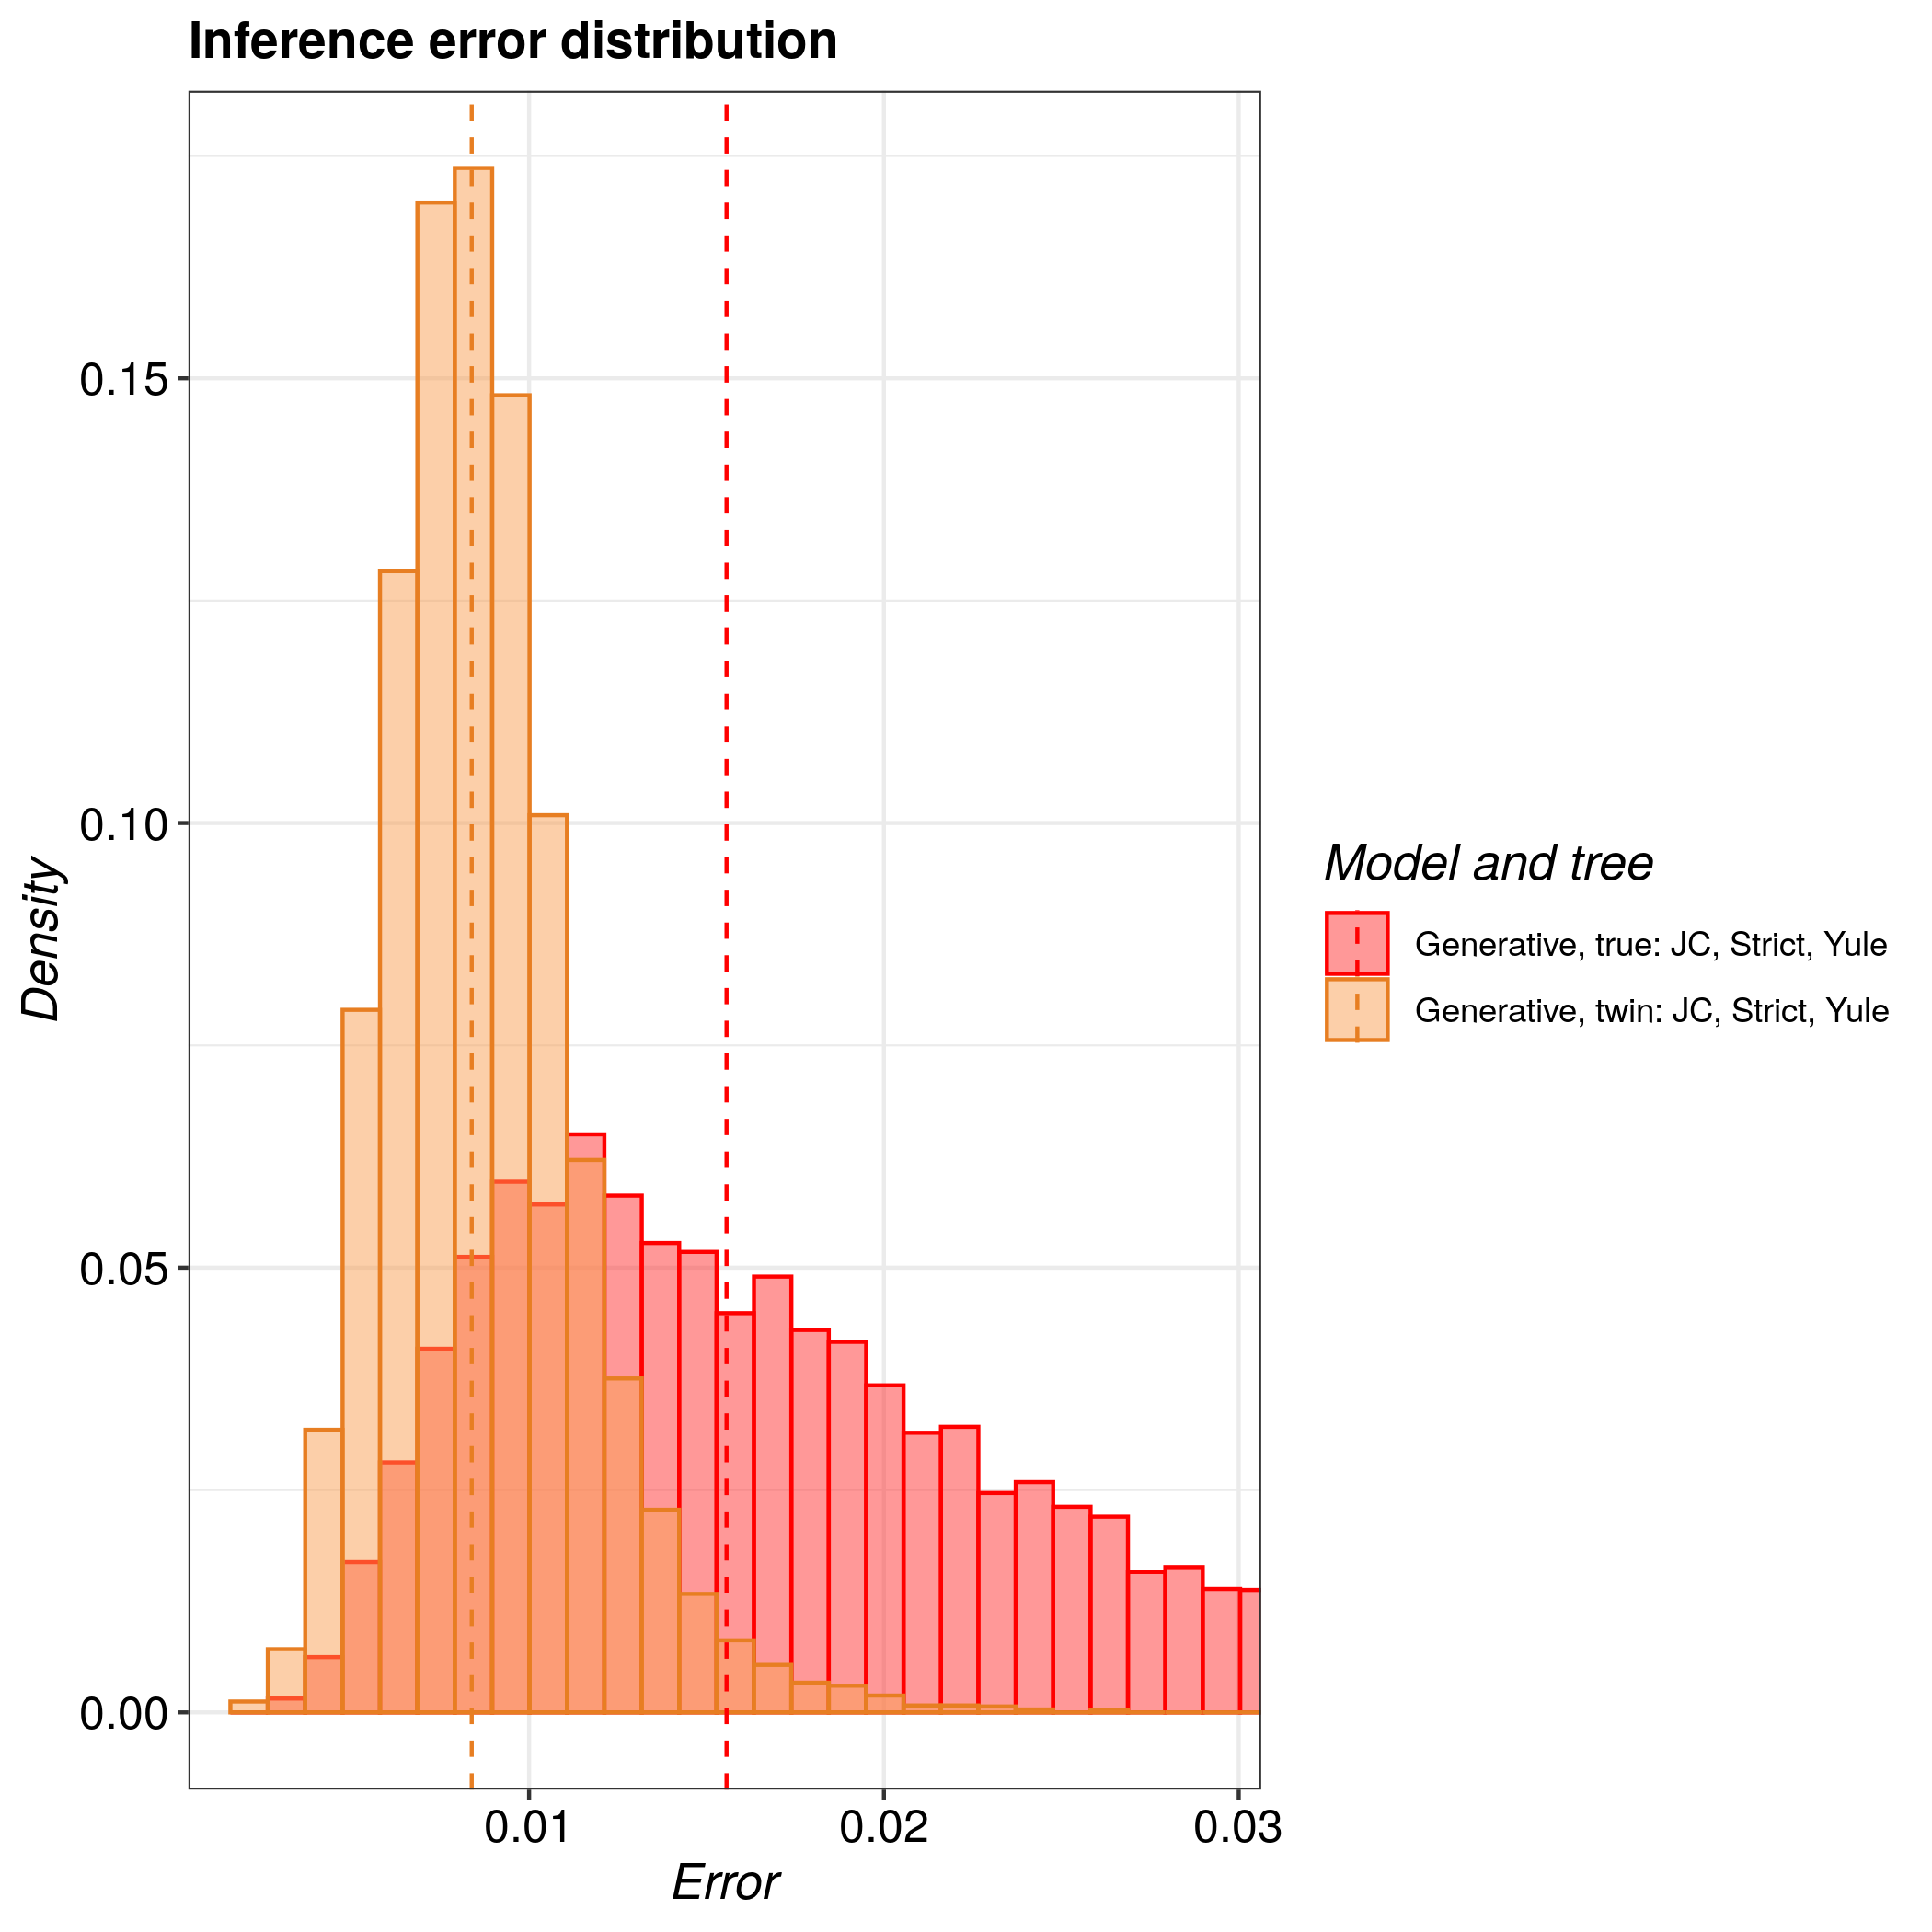
\includegraphics[width=\textwidth]{pirouette_example_20/example_20_314/errors.png}
  \caption{10 taxa}
\end{figure}

\begin{figure}[H]
  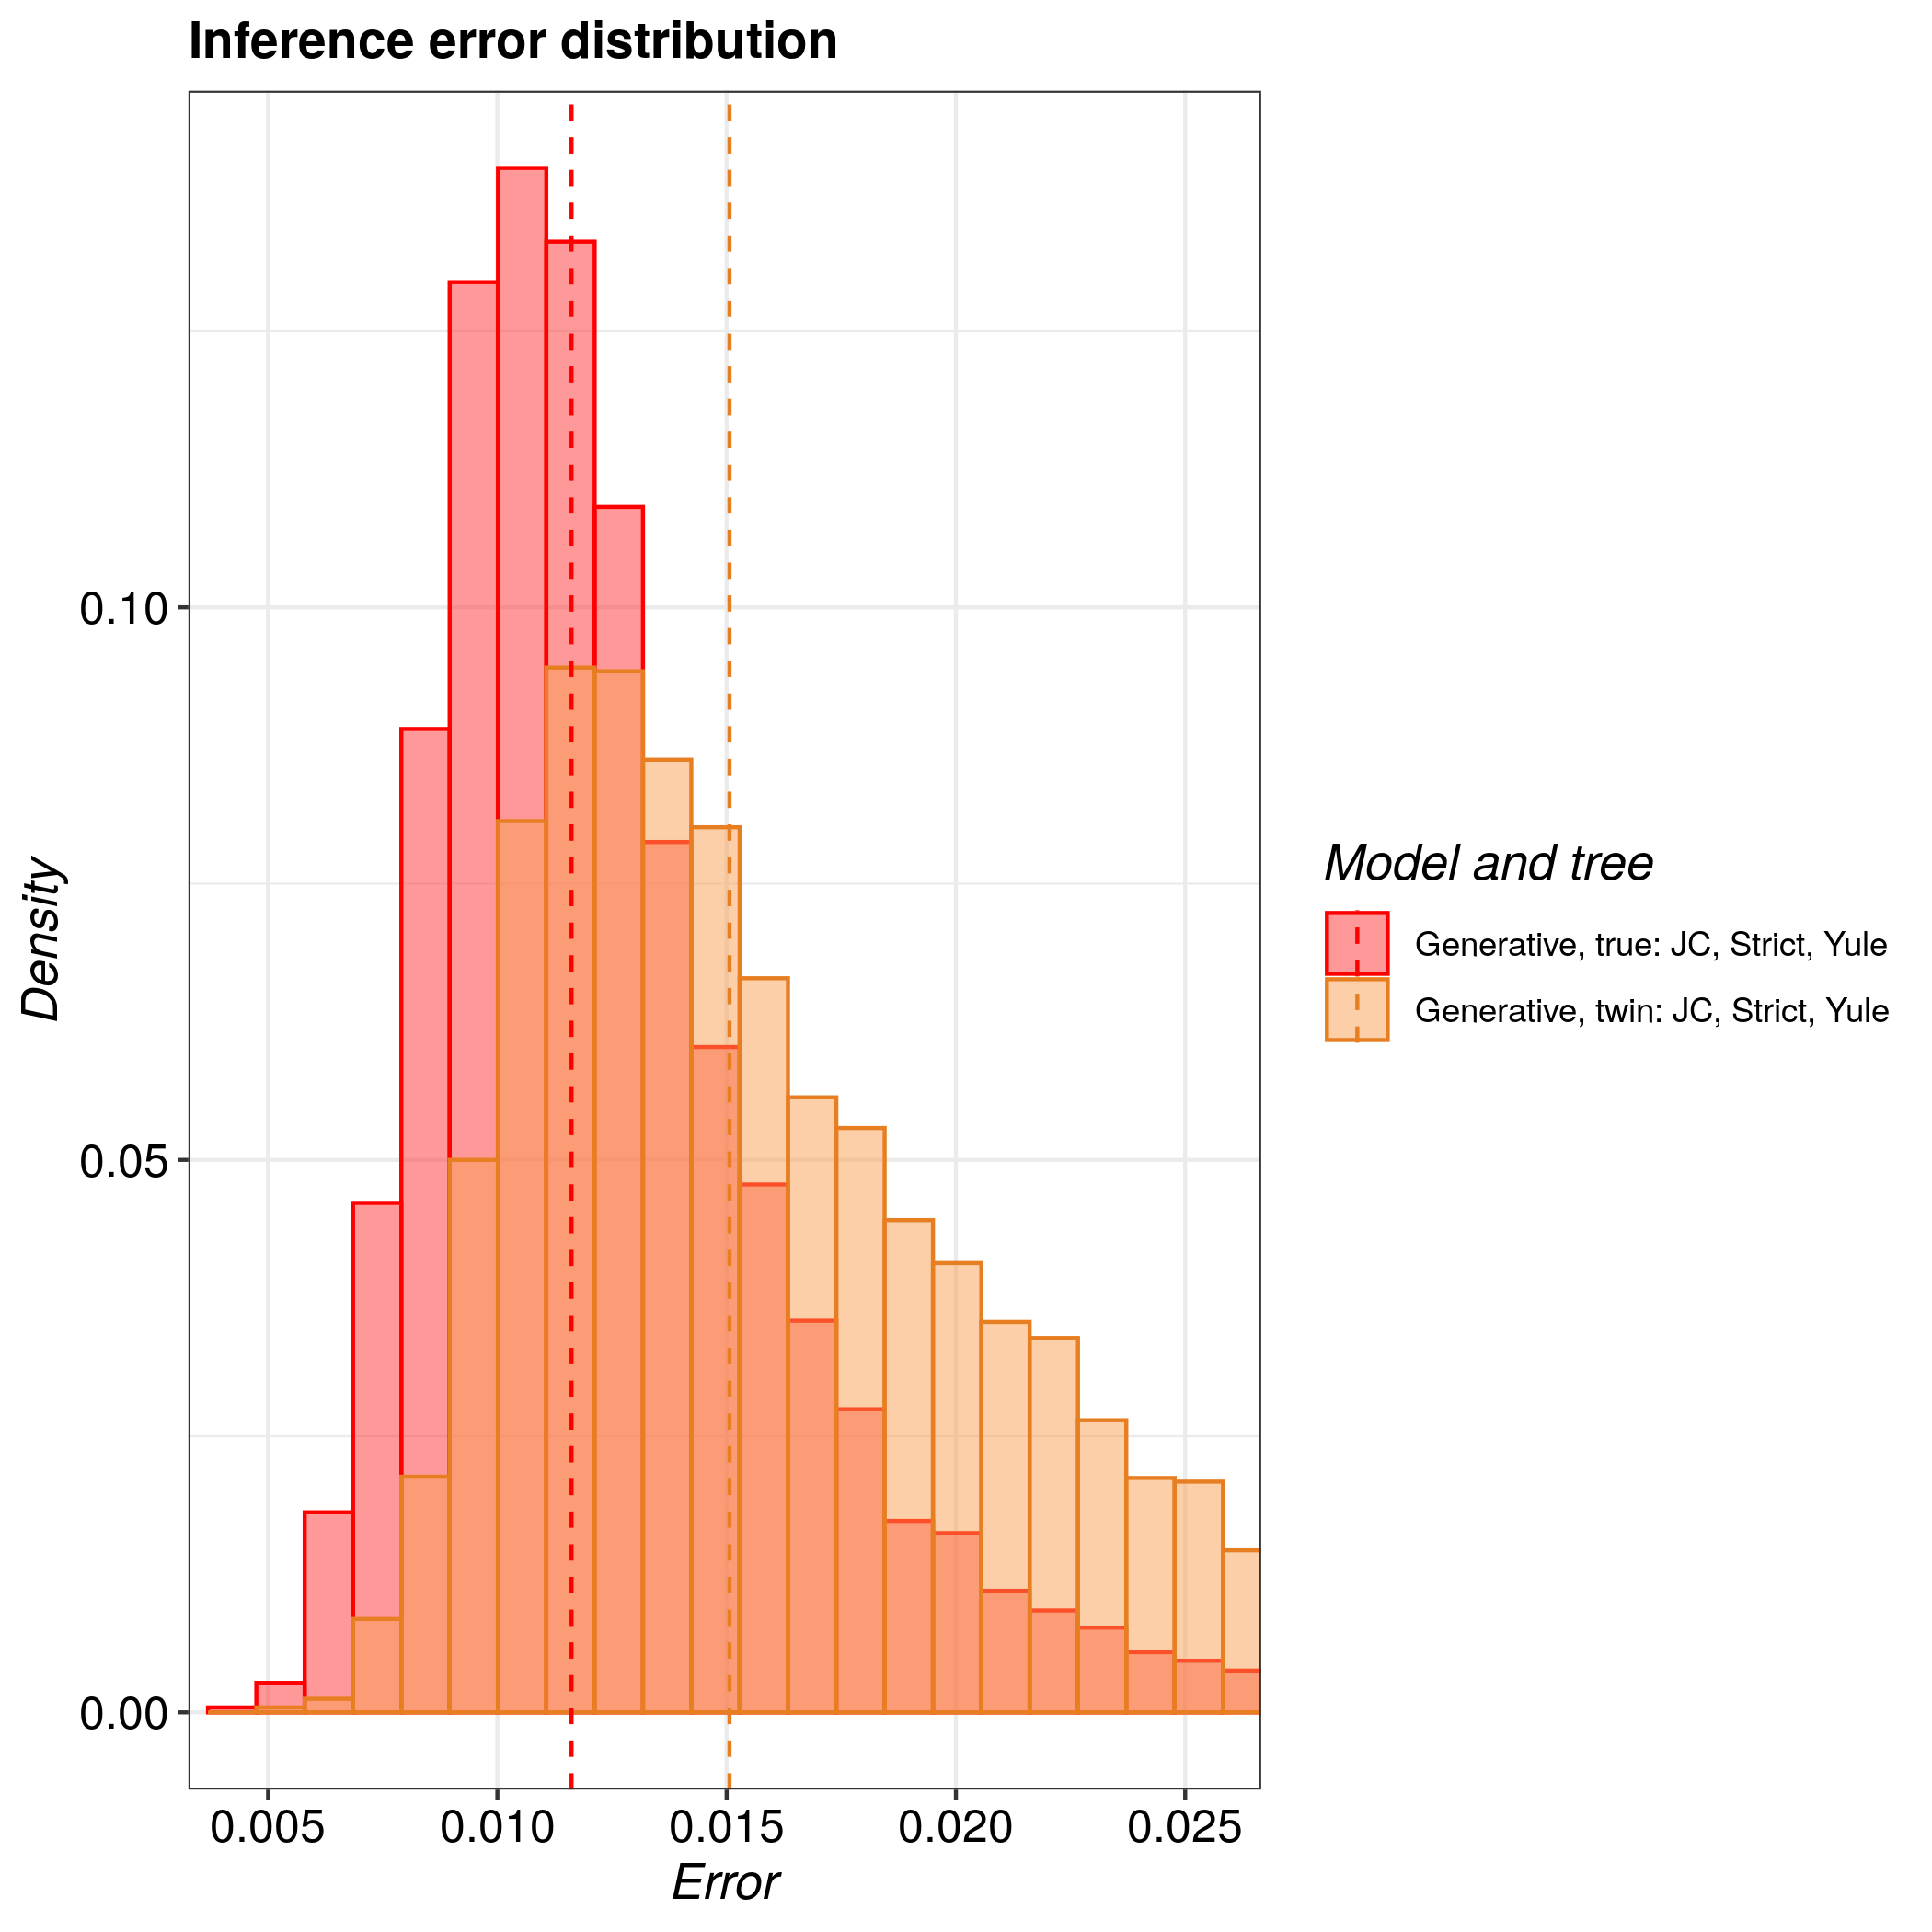
\includegraphics[width=\textwidth]{pirouette_example_20/example_20_315/errors.png}
  \caption{20 taxa}
\end{figure}

\begin{figure}[H]
  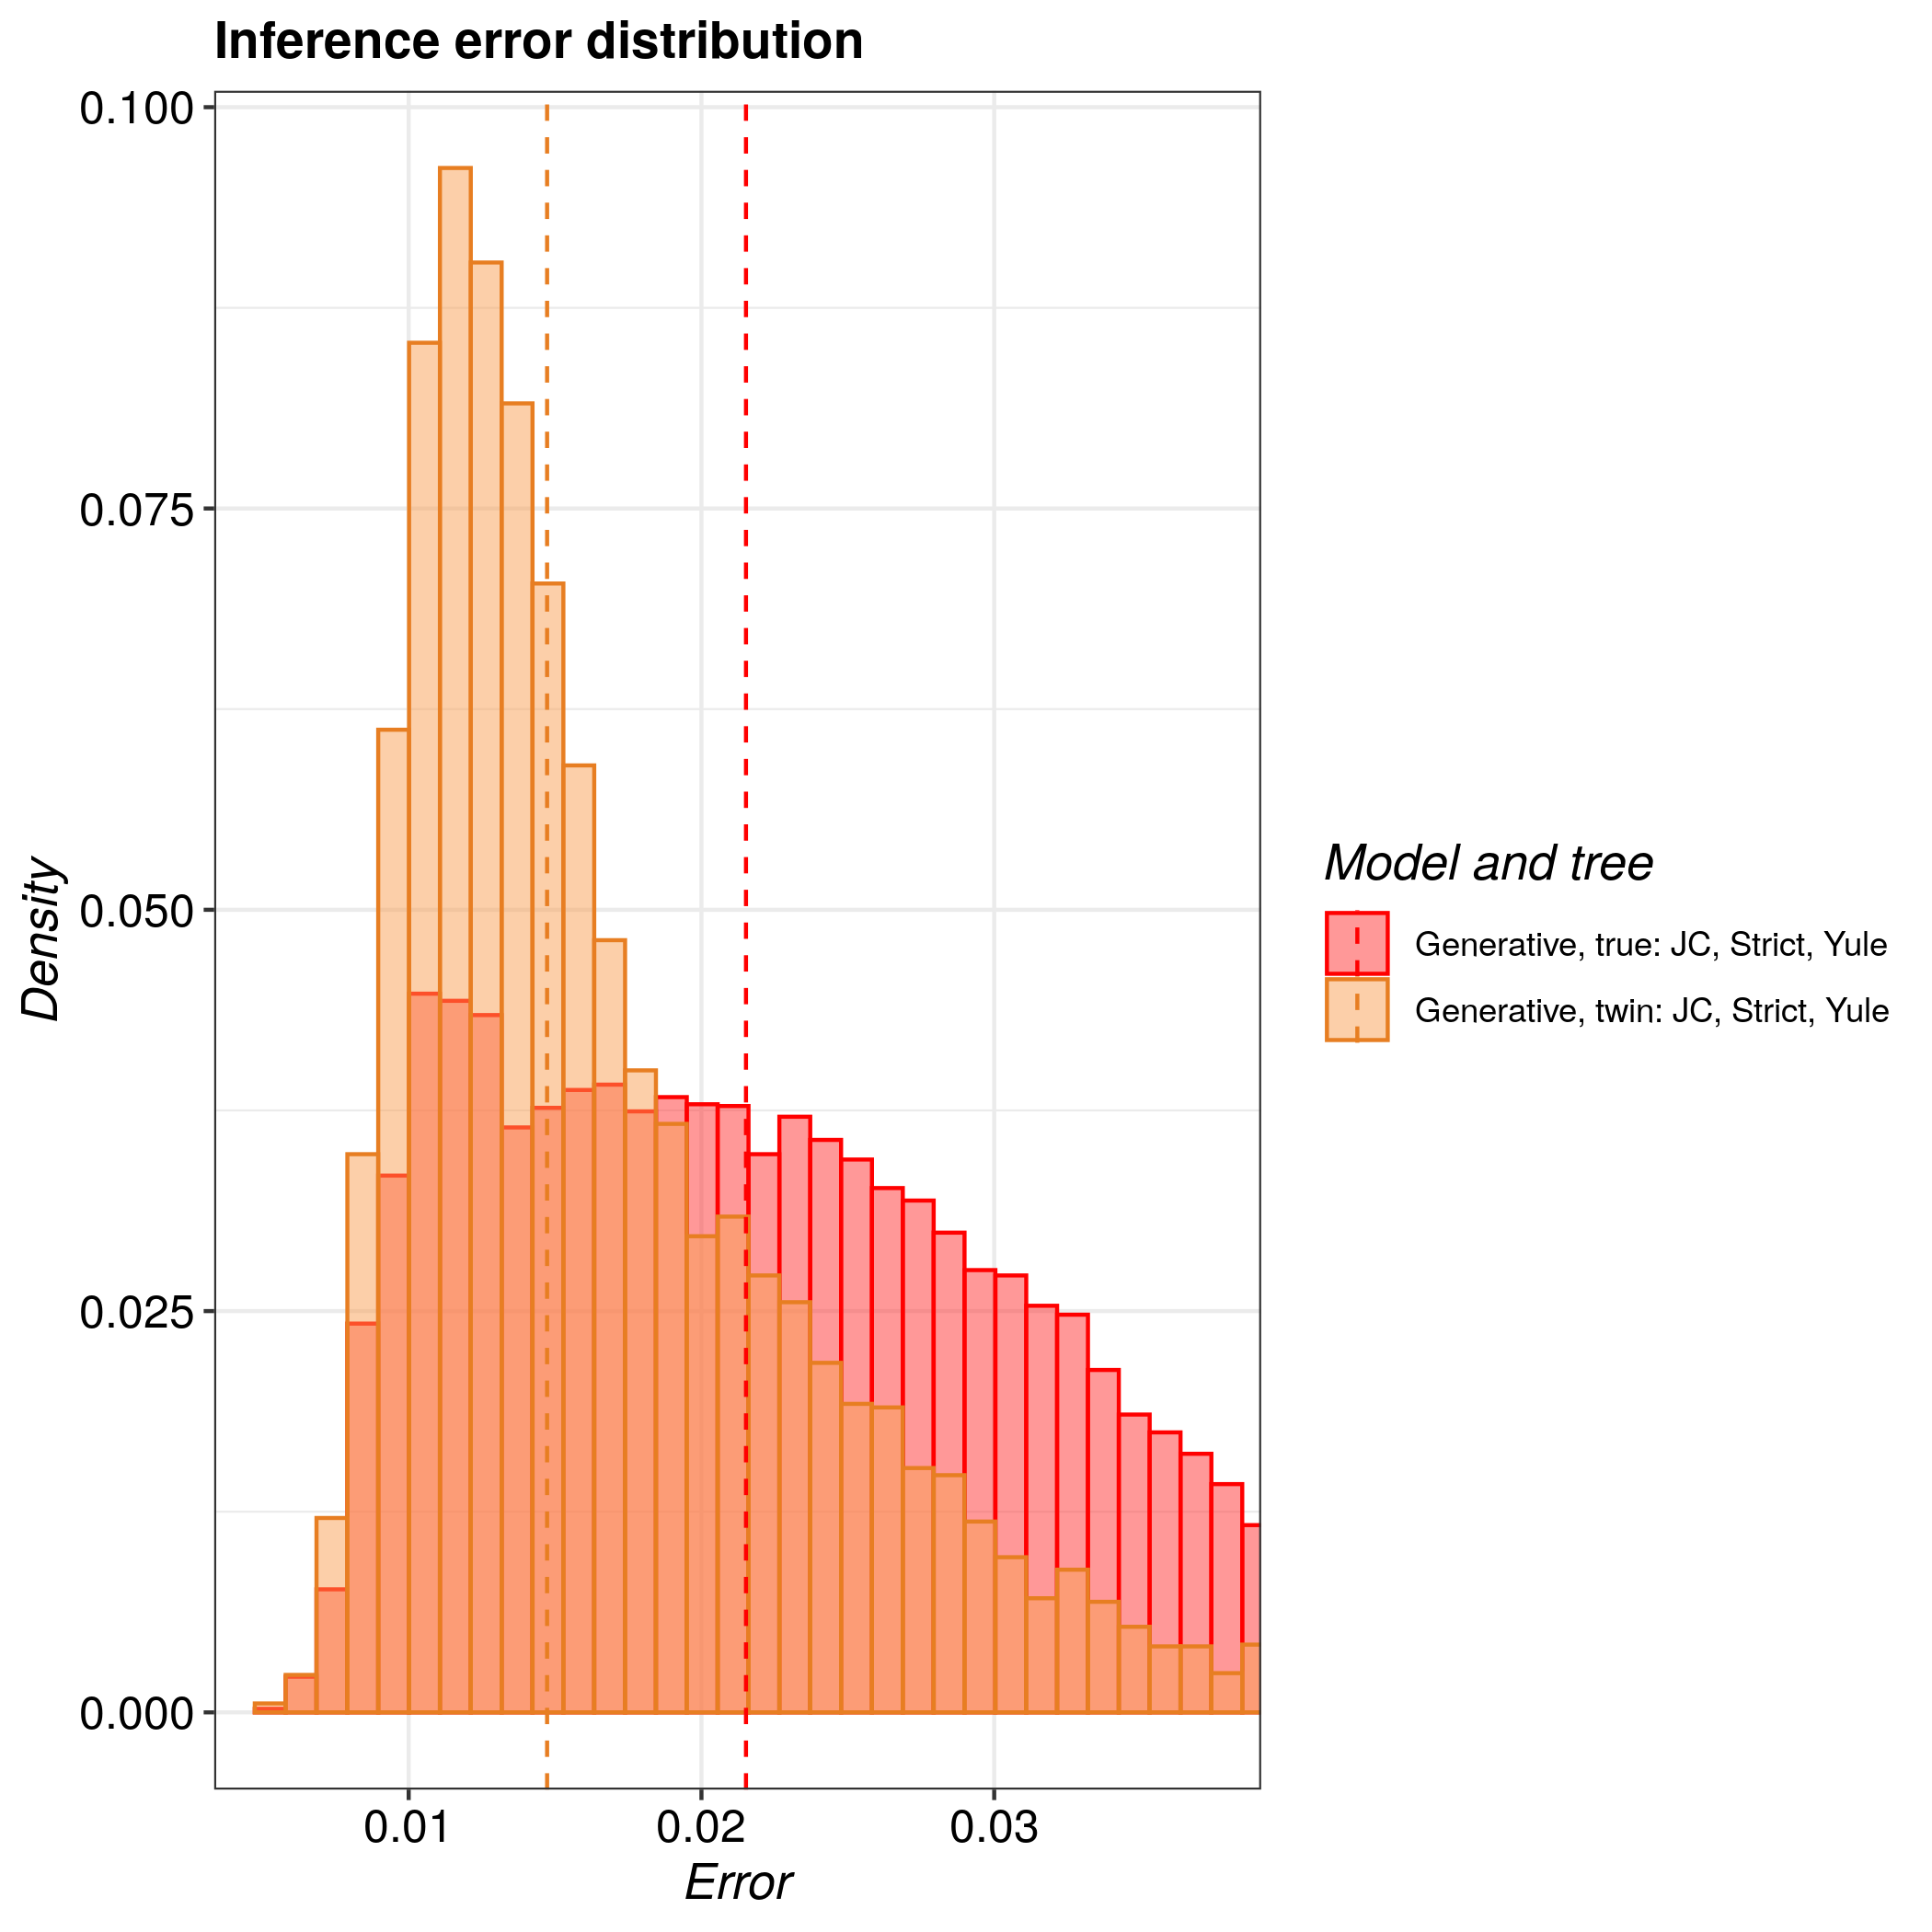
\includegraphics[width=\textwidth]{pirouette_example_20/example_20_316/errors.png}
  \caption{30 taxa}
\end{figure}

\begin{figure}[H]
  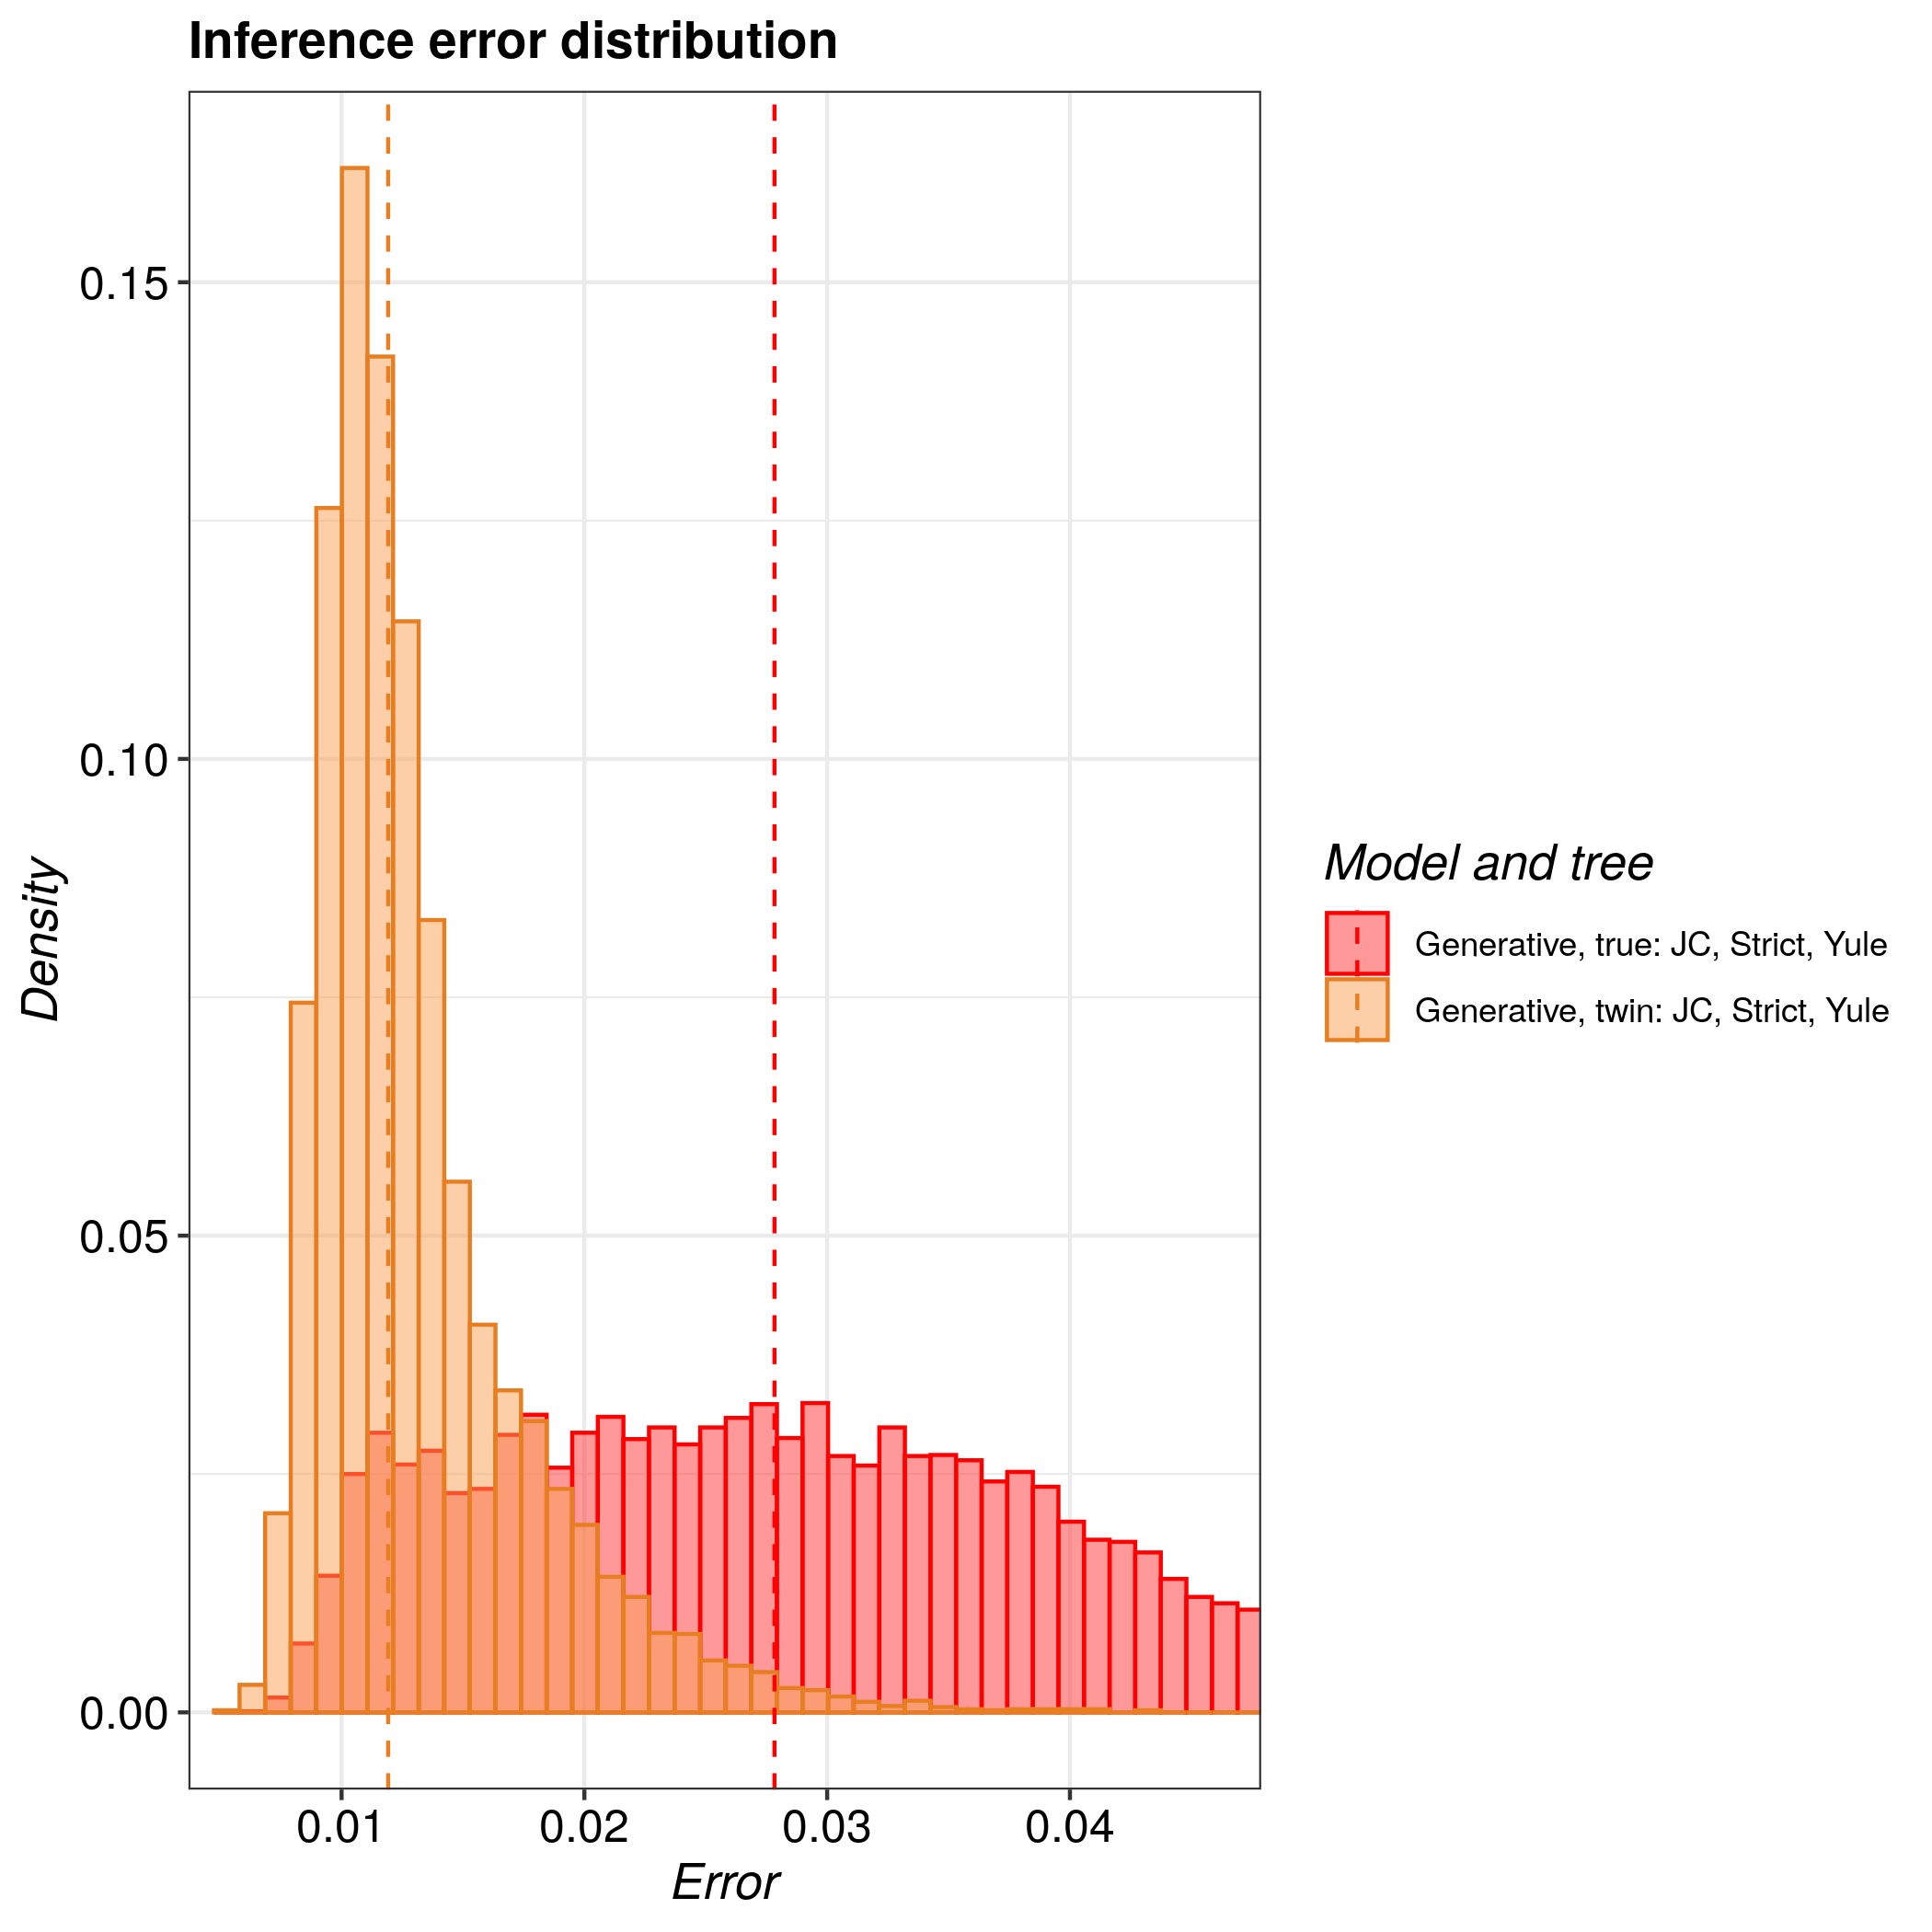
\includegraphics[width=\textwidth]{pirouette_example_20/example_20_317/errors.png}
  \caption{40 taxa}
\end{figure}

%%%%%%%%%%%%%%%%%%%%%%%%%%%%%%%%%%%%%%%%%%%%%%%%%%%%%%%%%%%%%%%%%%%%%%%%%%%%%%%%
\subsection{The effect of DNA sequence length}
%%%%%%%%%%%%%%%%%%%%%%%%%%%%%%%%%%%%%%%%%%%%%%%%%%%%%%%%%%%%%%%%%%%%%%%%%%%%%%%%

The code used in this part of the article can be found at 
\url{https://github.com/richelbilderbeek/pirouette_example_21}.

\begin{figure}[H]
  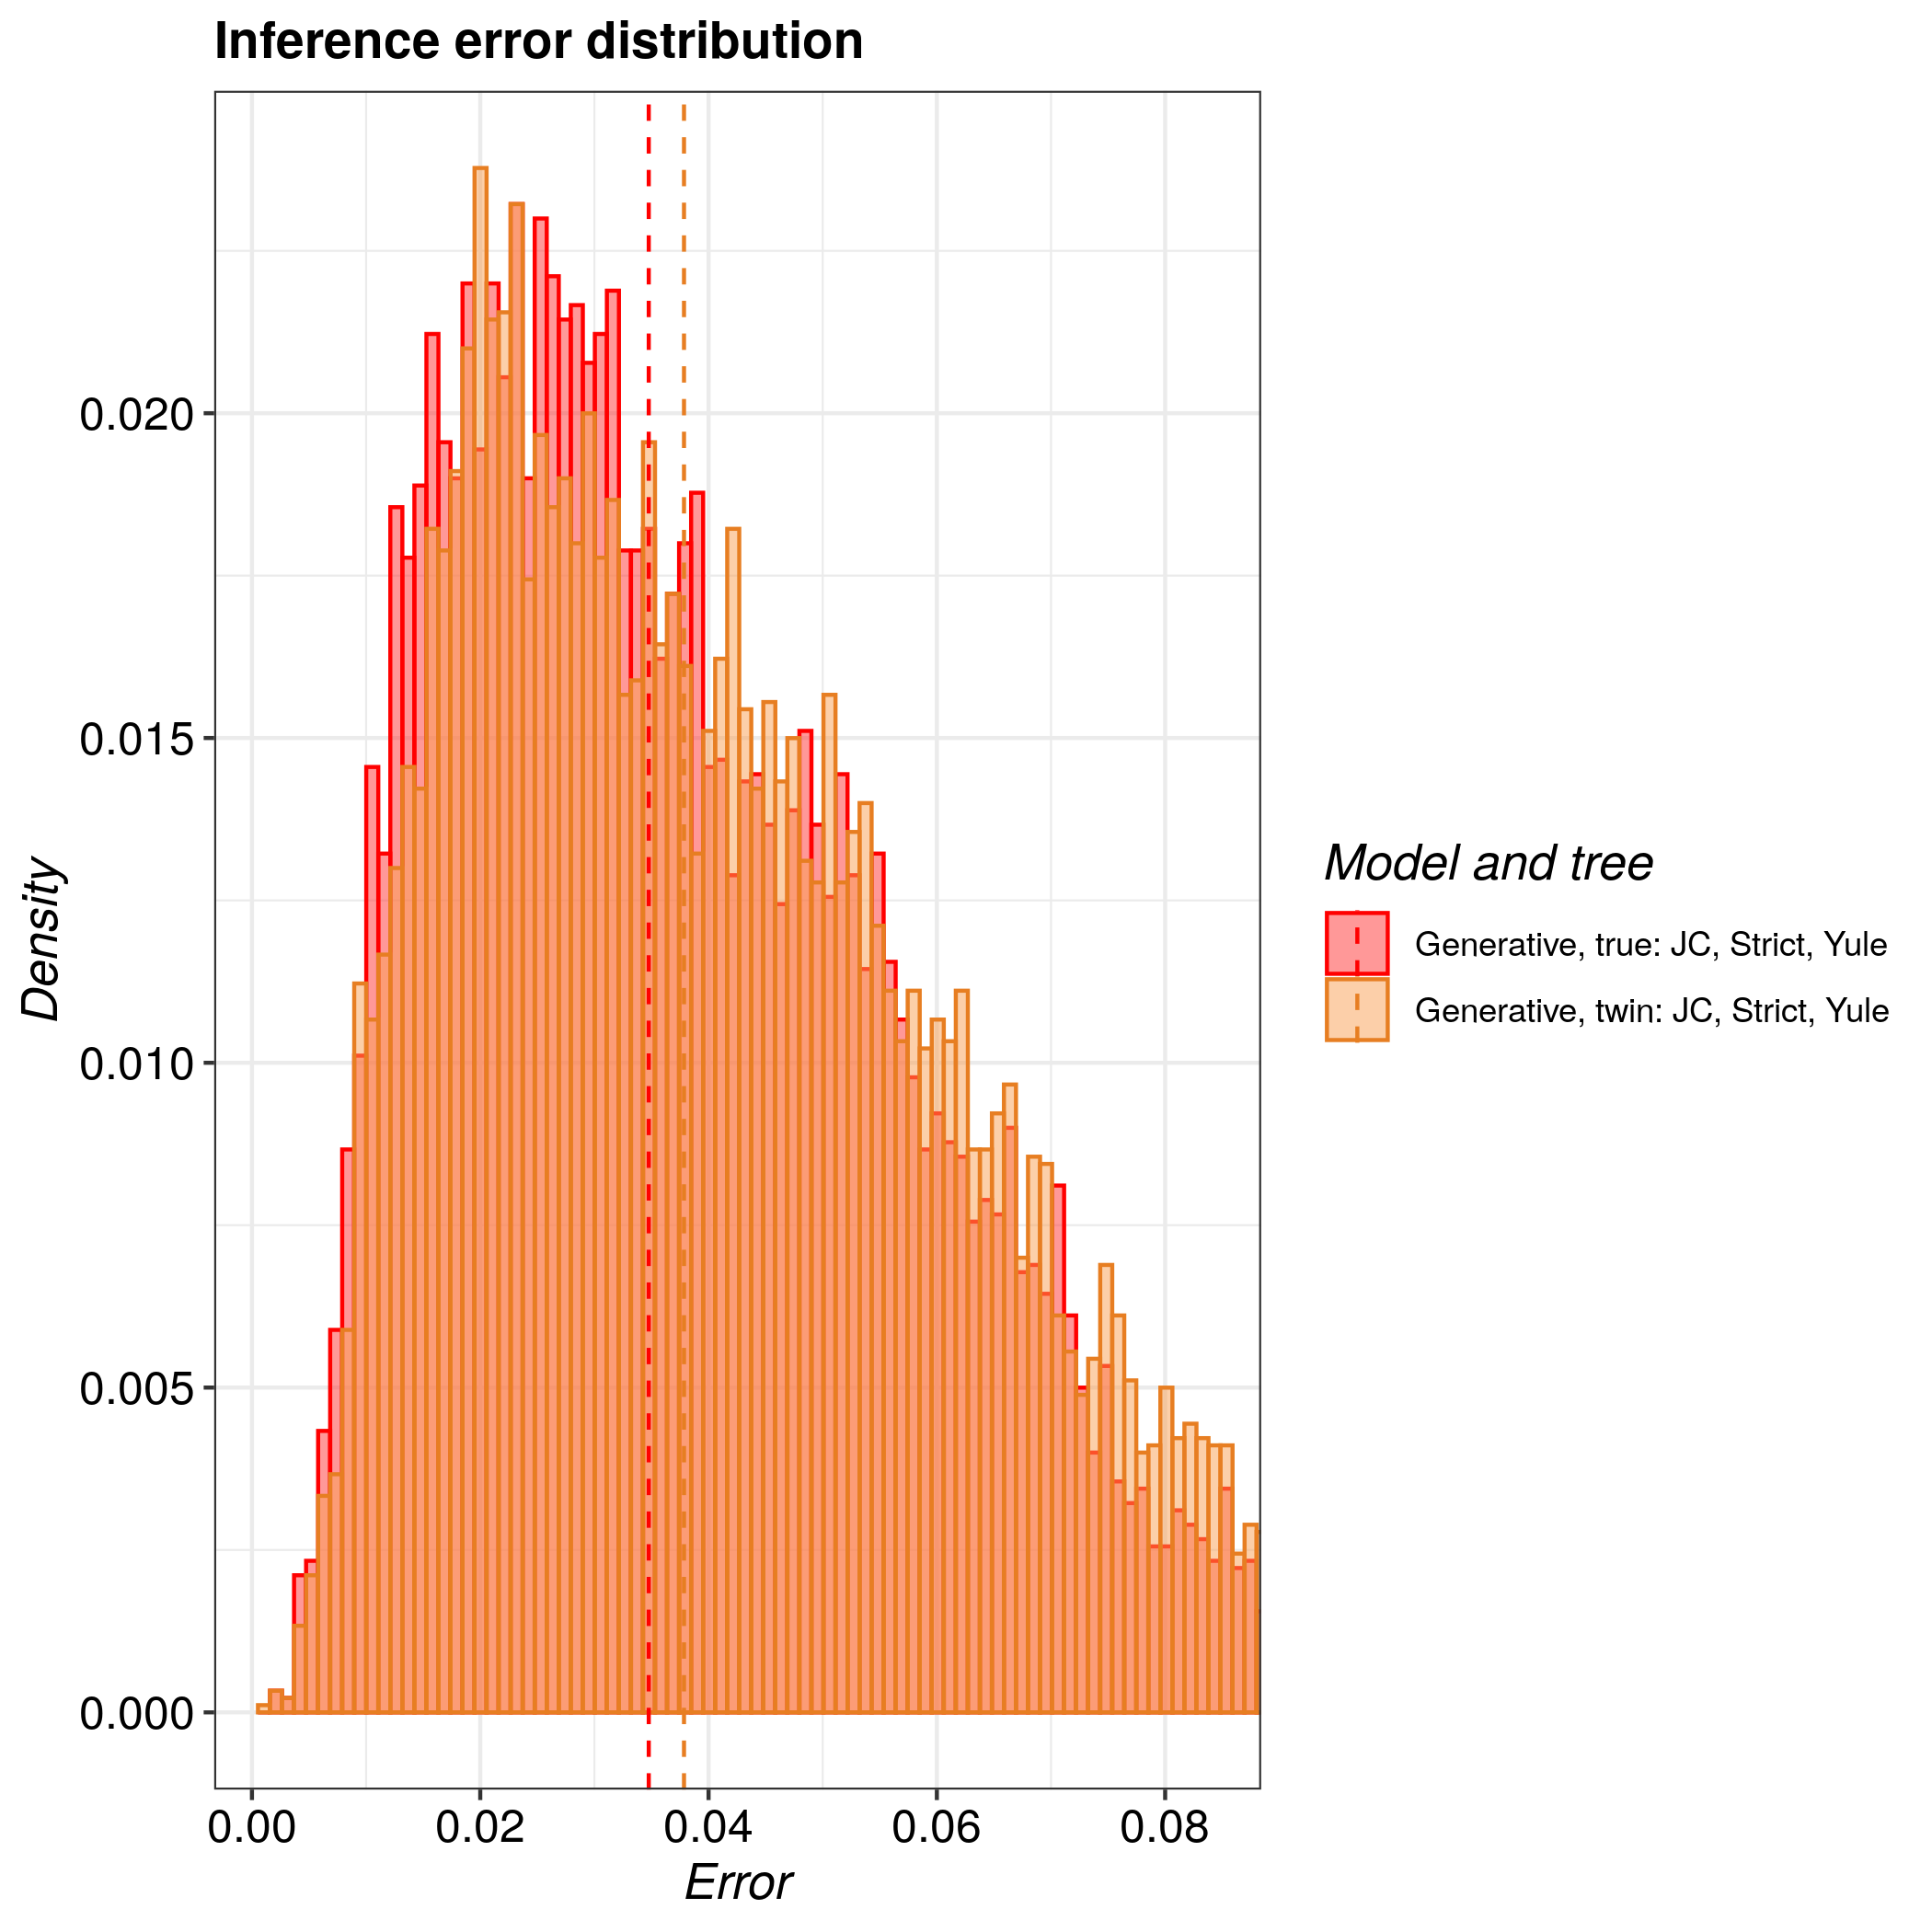
\includegraphics[width=\textwidth]{pirouette_example_21/example_21_314/errors.png}
  \caption{100 nucleotides}
\end{figure}

\begin{figure}[H]
  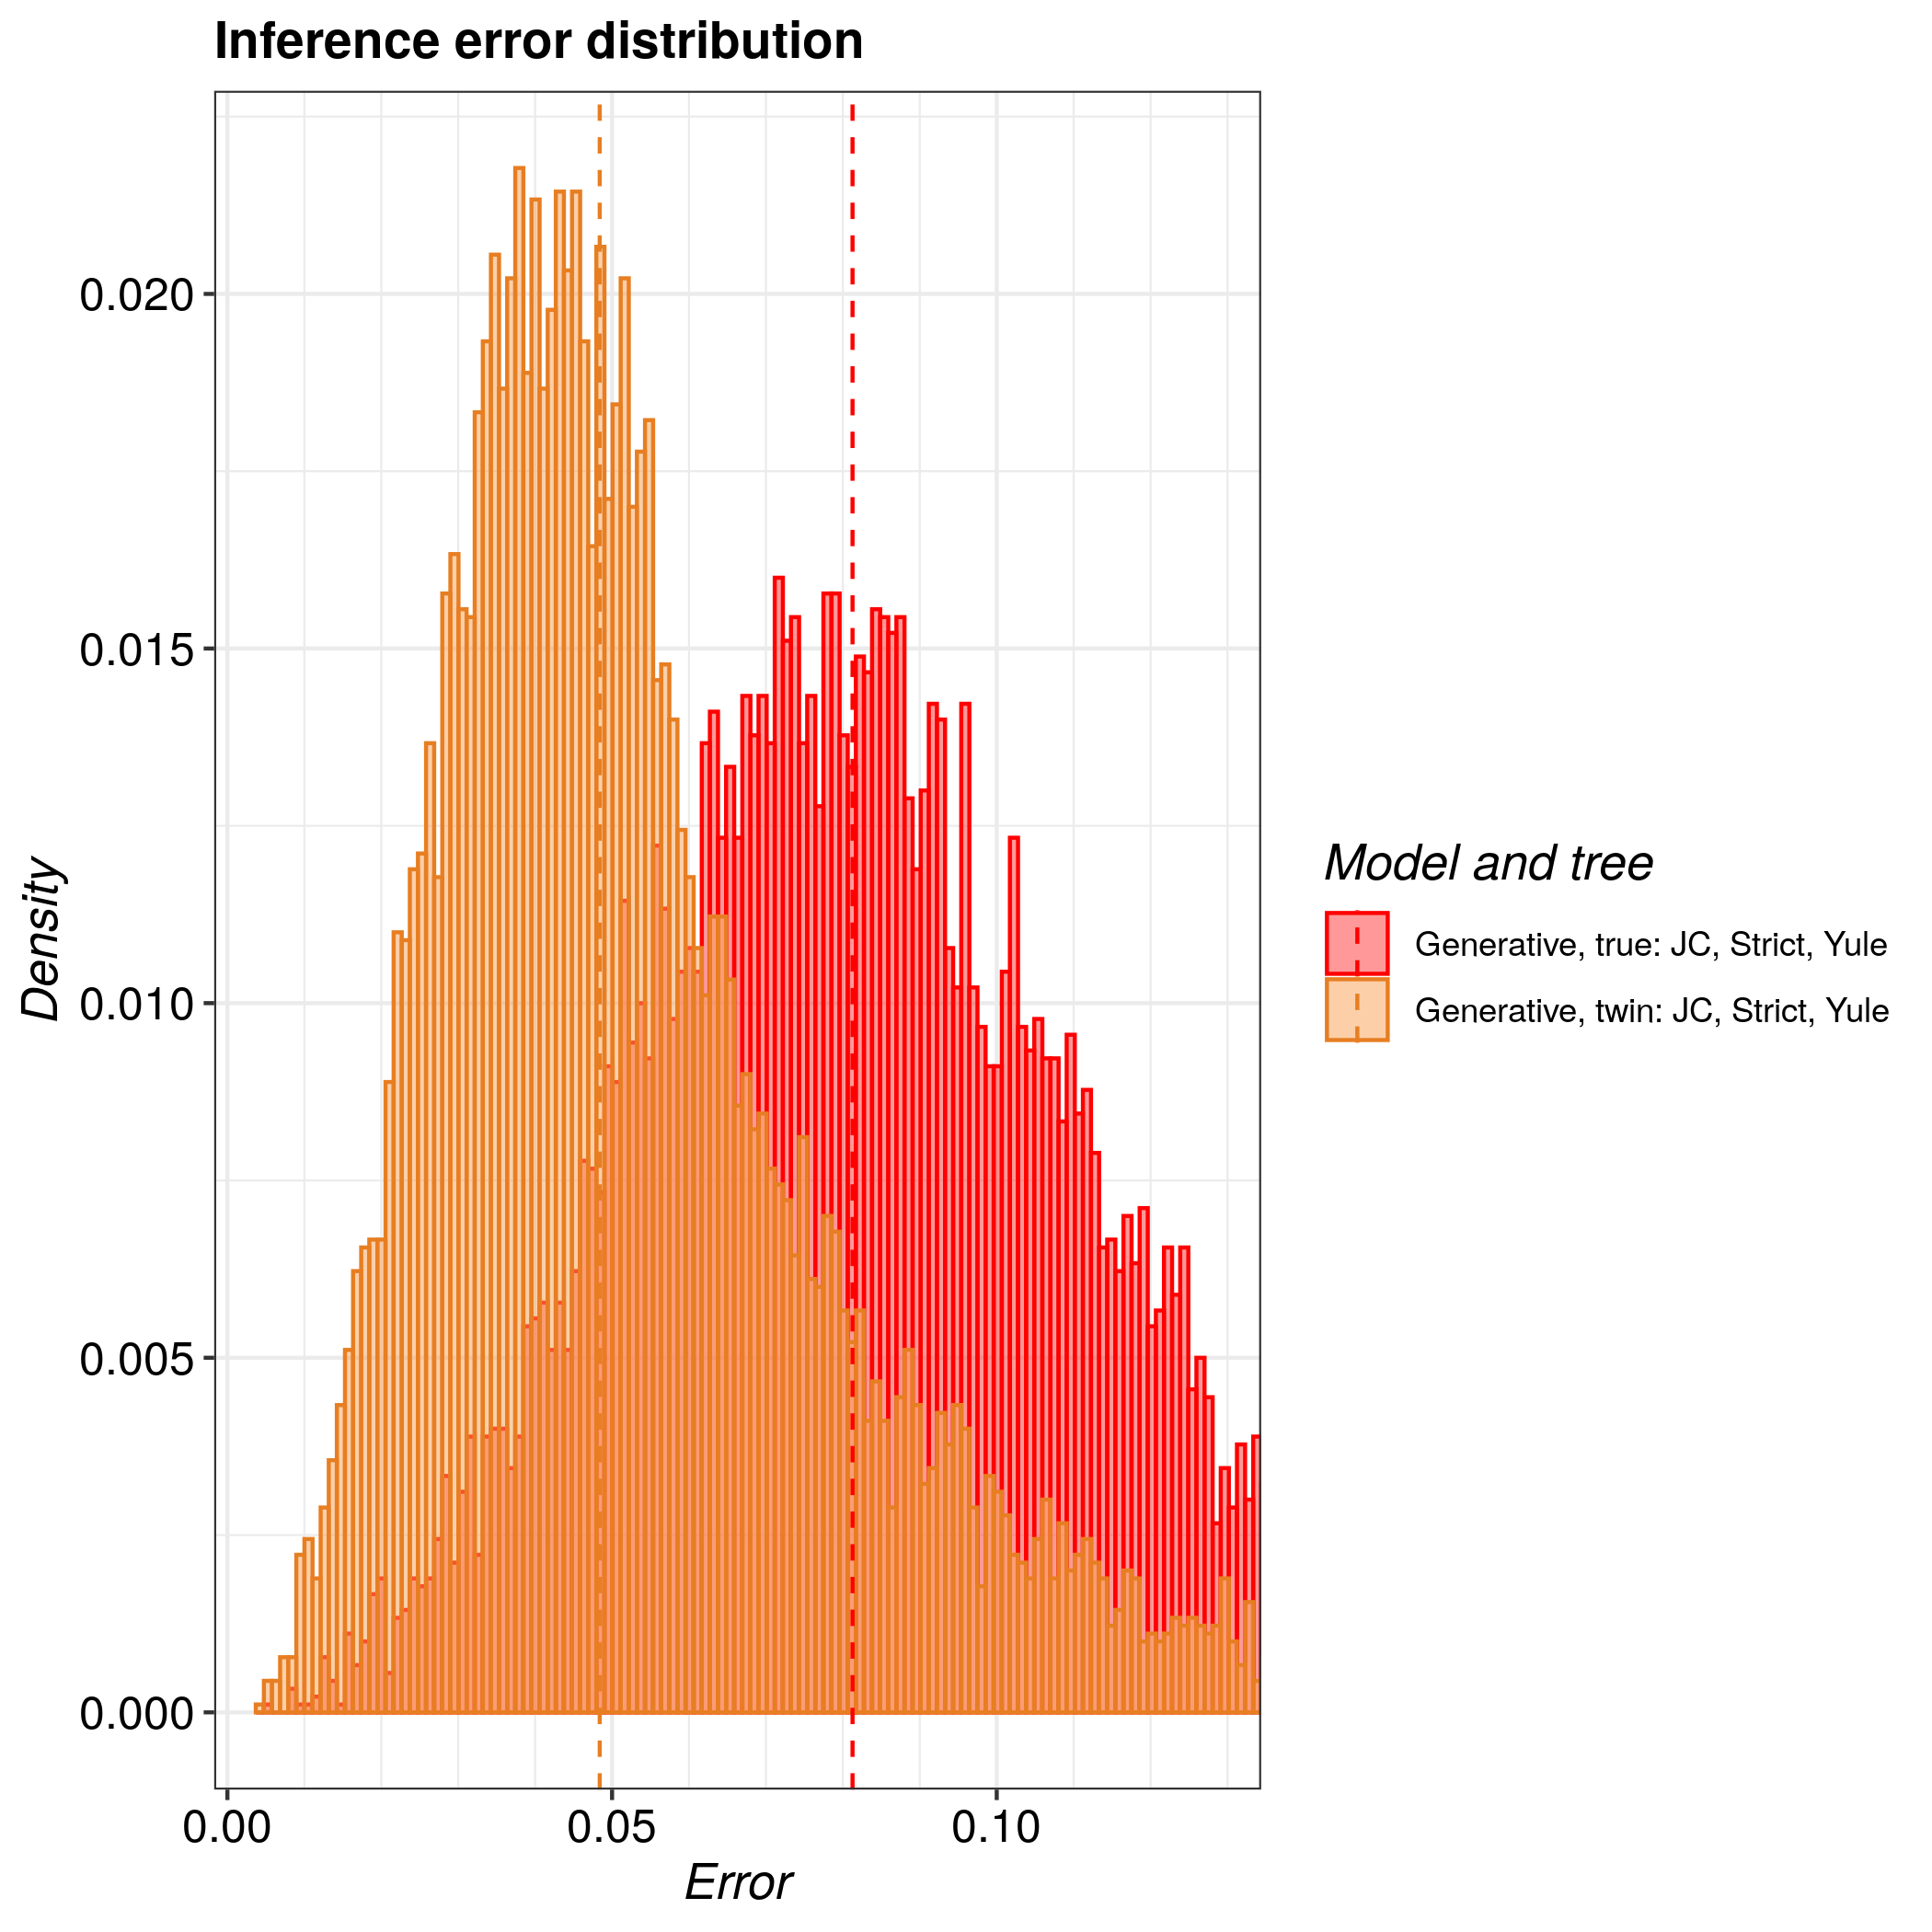
\includegraphics[width=\textwidth]{pirouette_example_21/example_21_315/errors.png}
  \caption{248 nucleotides}
\end{figure}

\begin{figure}[H]
  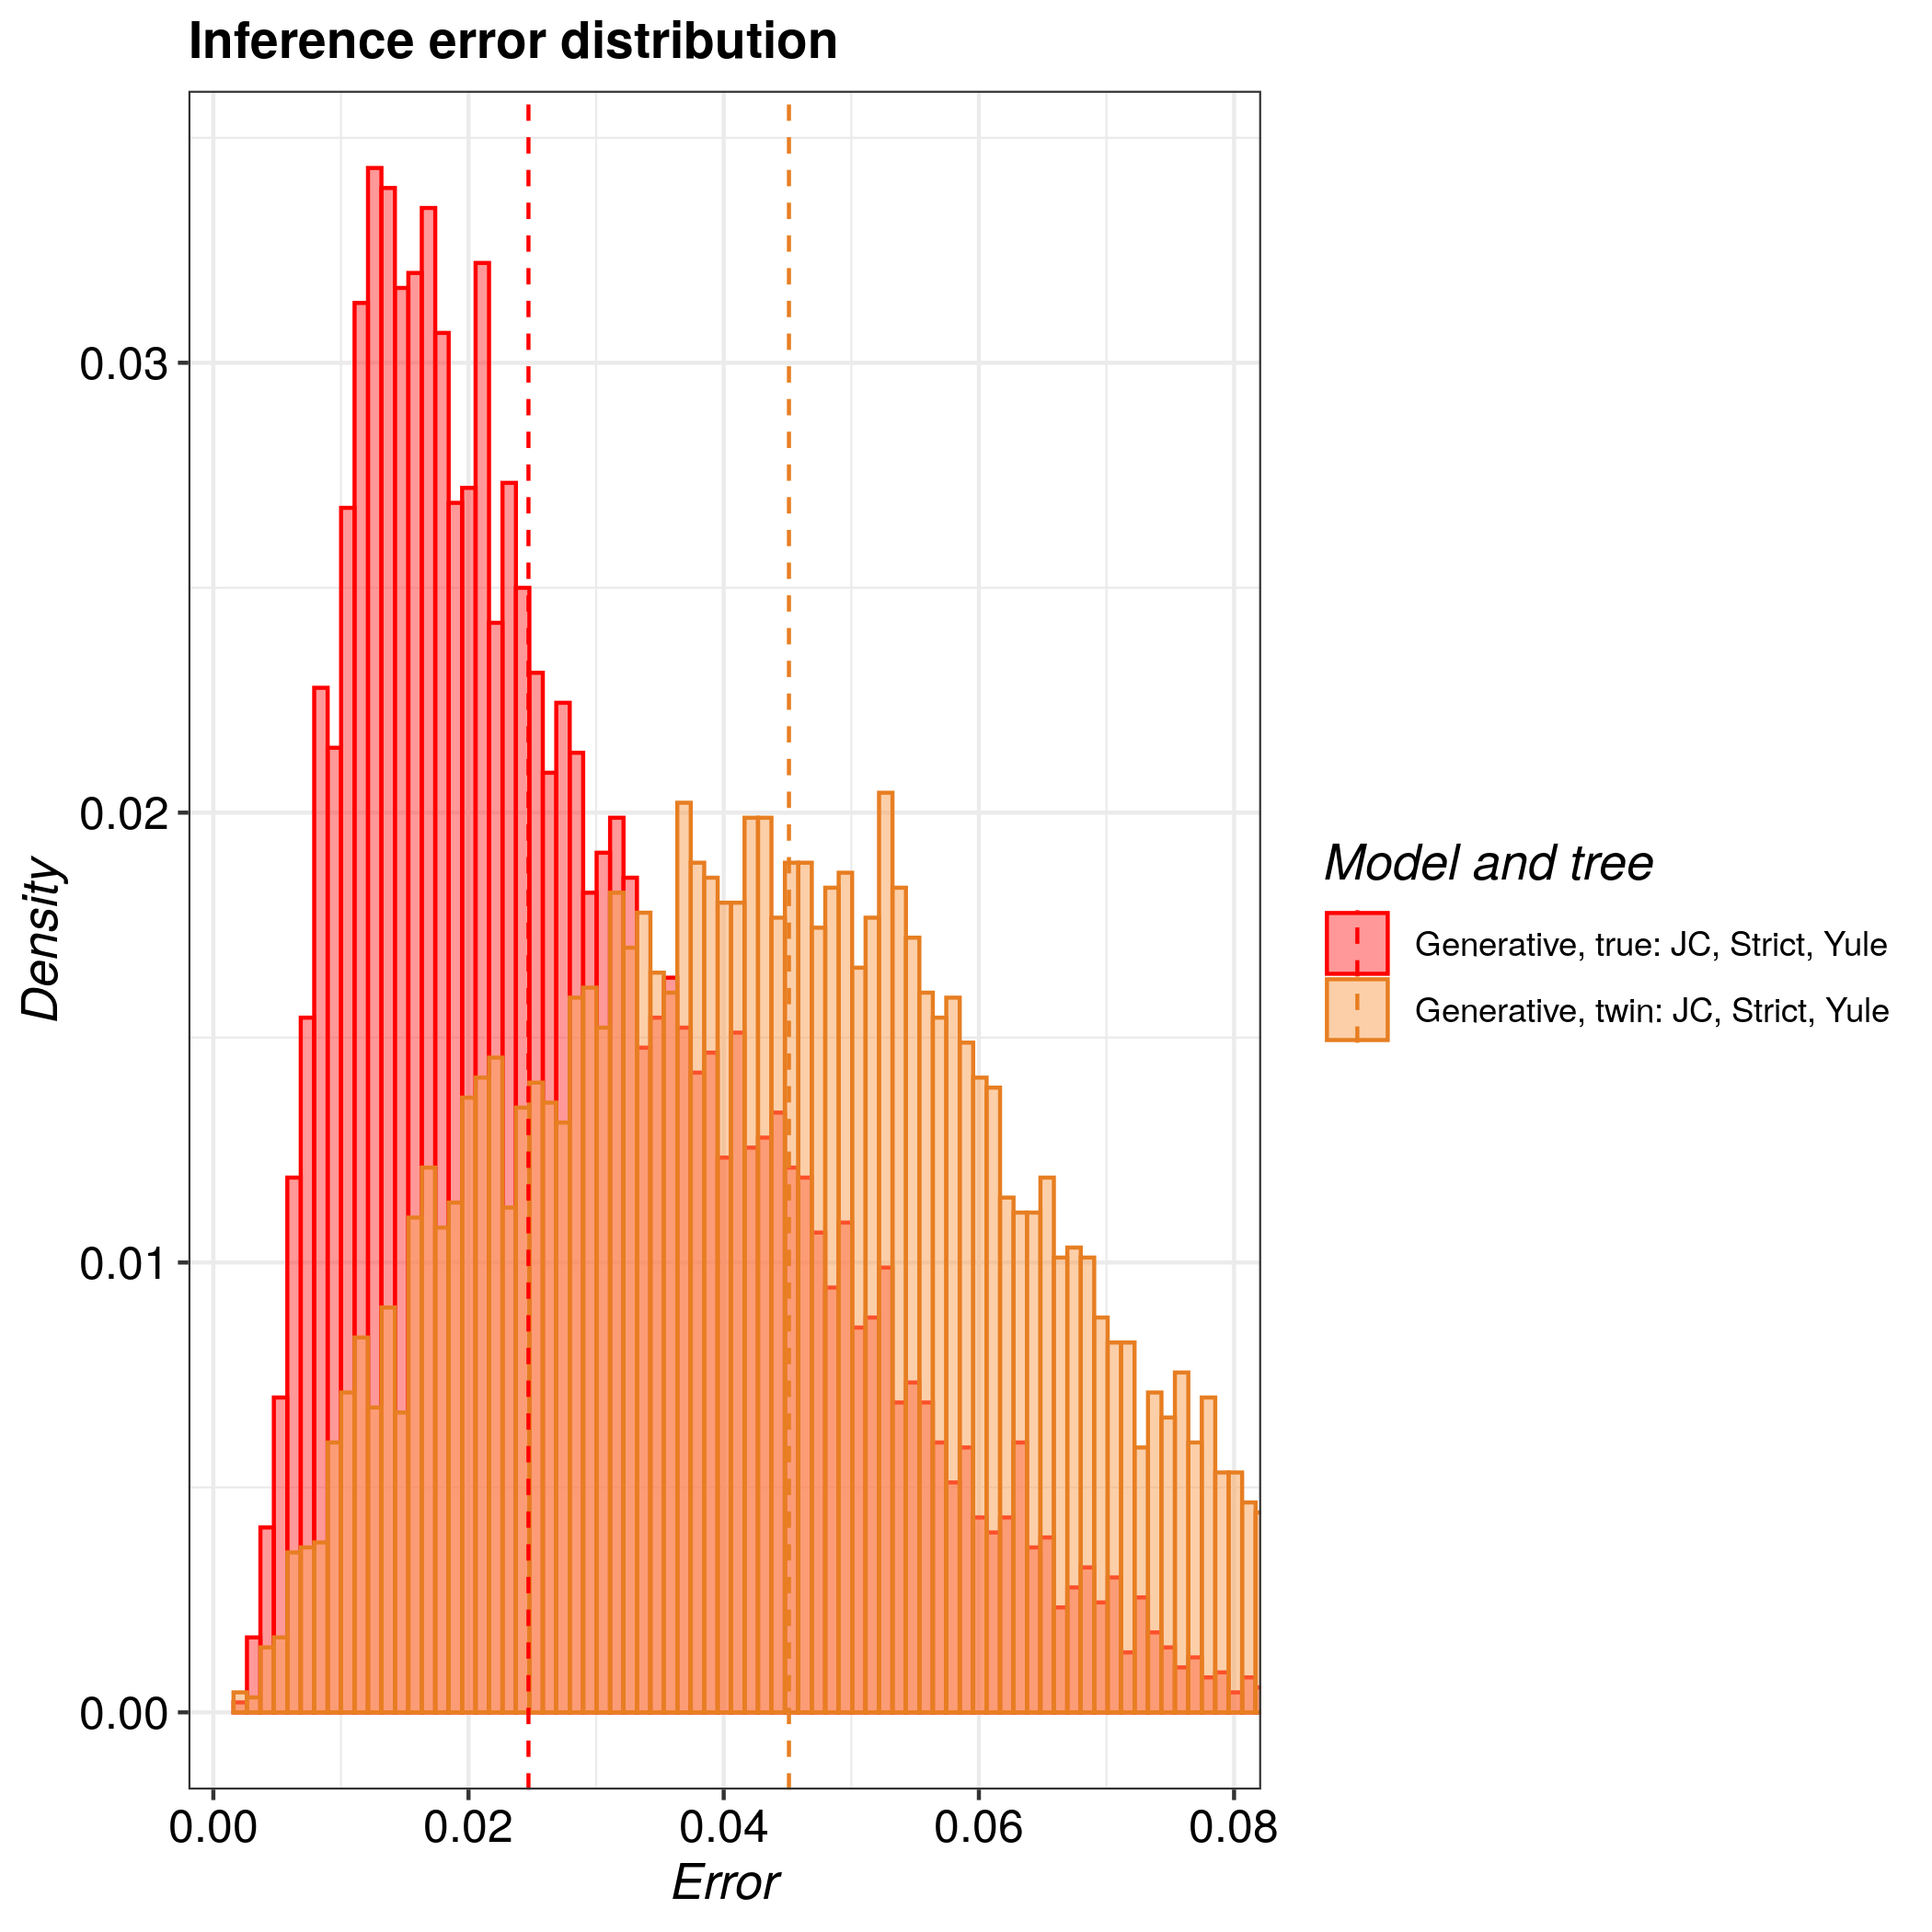
\includegraphics[width=\textwidth]{pirouette_example_21/example_21_316/errors.png}
  \caption{500 nucleotides}
\end{figure}

\begin{figure}[H]
  \includegraphics[width=\textwidth]{pirouette_example_21/example_21_317/errors.png}
  \caption{1000 nucleotides}
\end{figure}

\begin{figure}[H]
  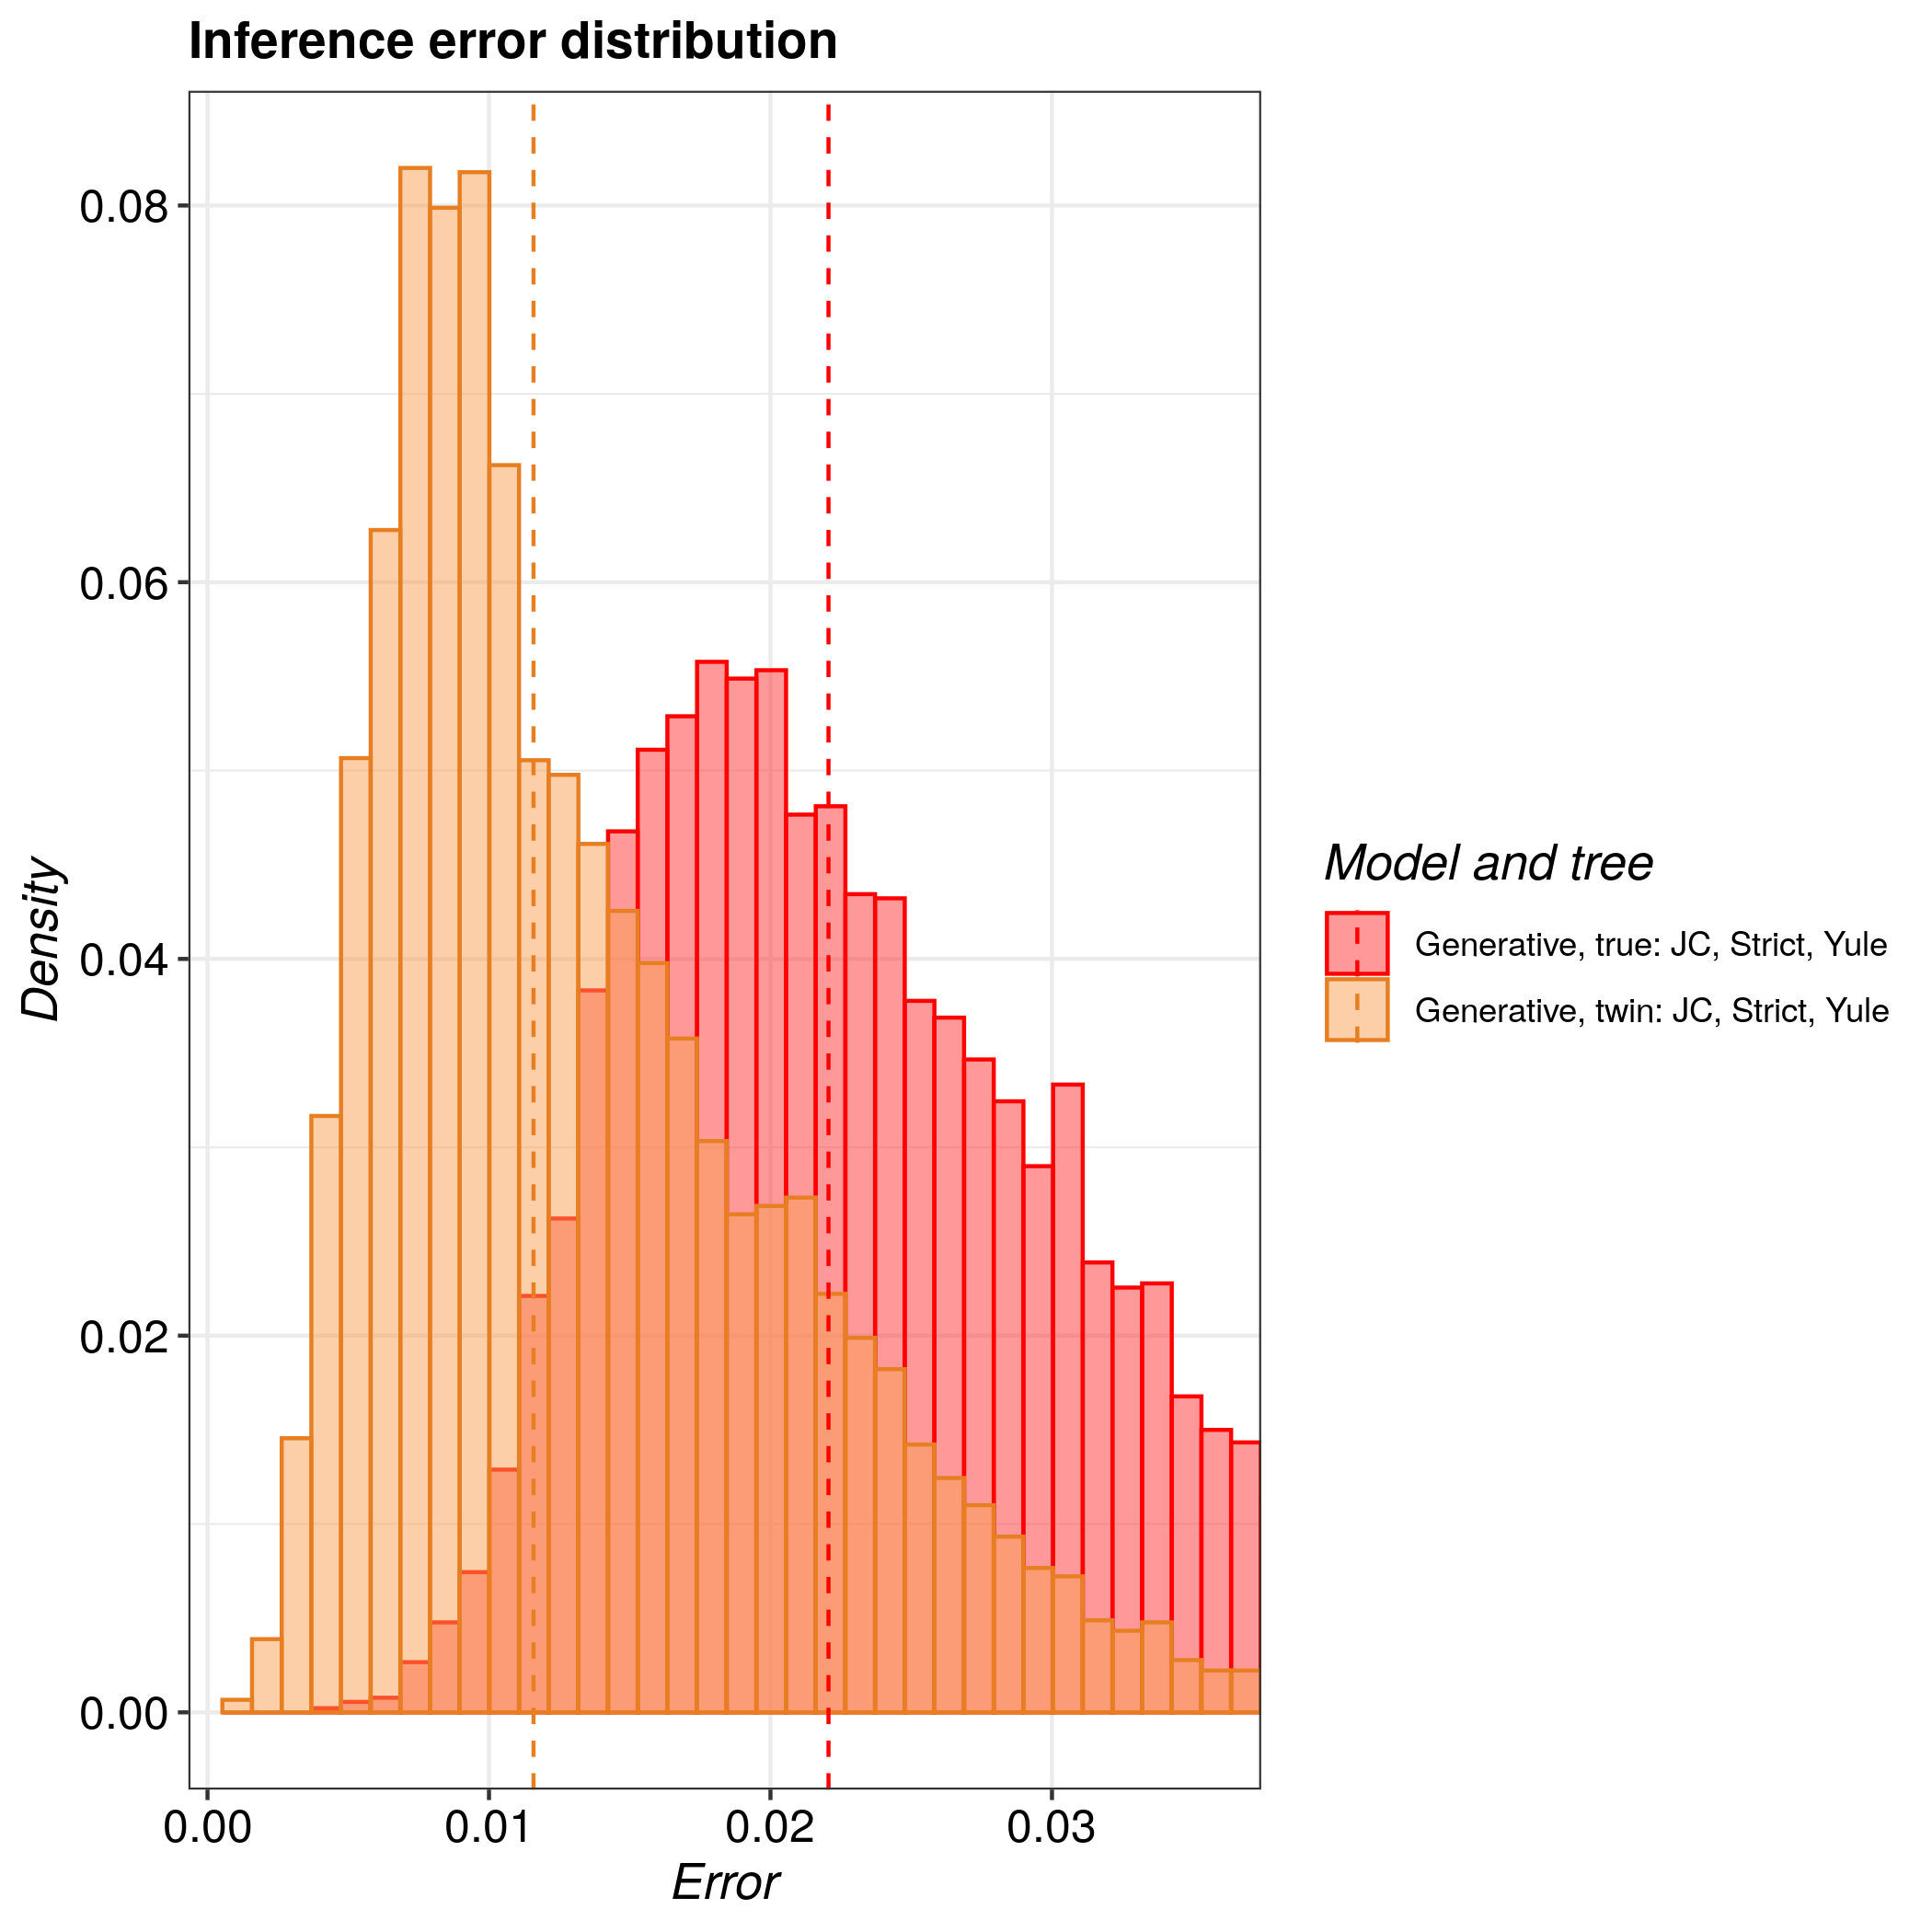
\includegraphics[width=\textwidth]{pirouette_example_21/example_21_318/errors.png}
  \caption{2000 nucleotides}
\end{figure}

\begin{figure}[H]
  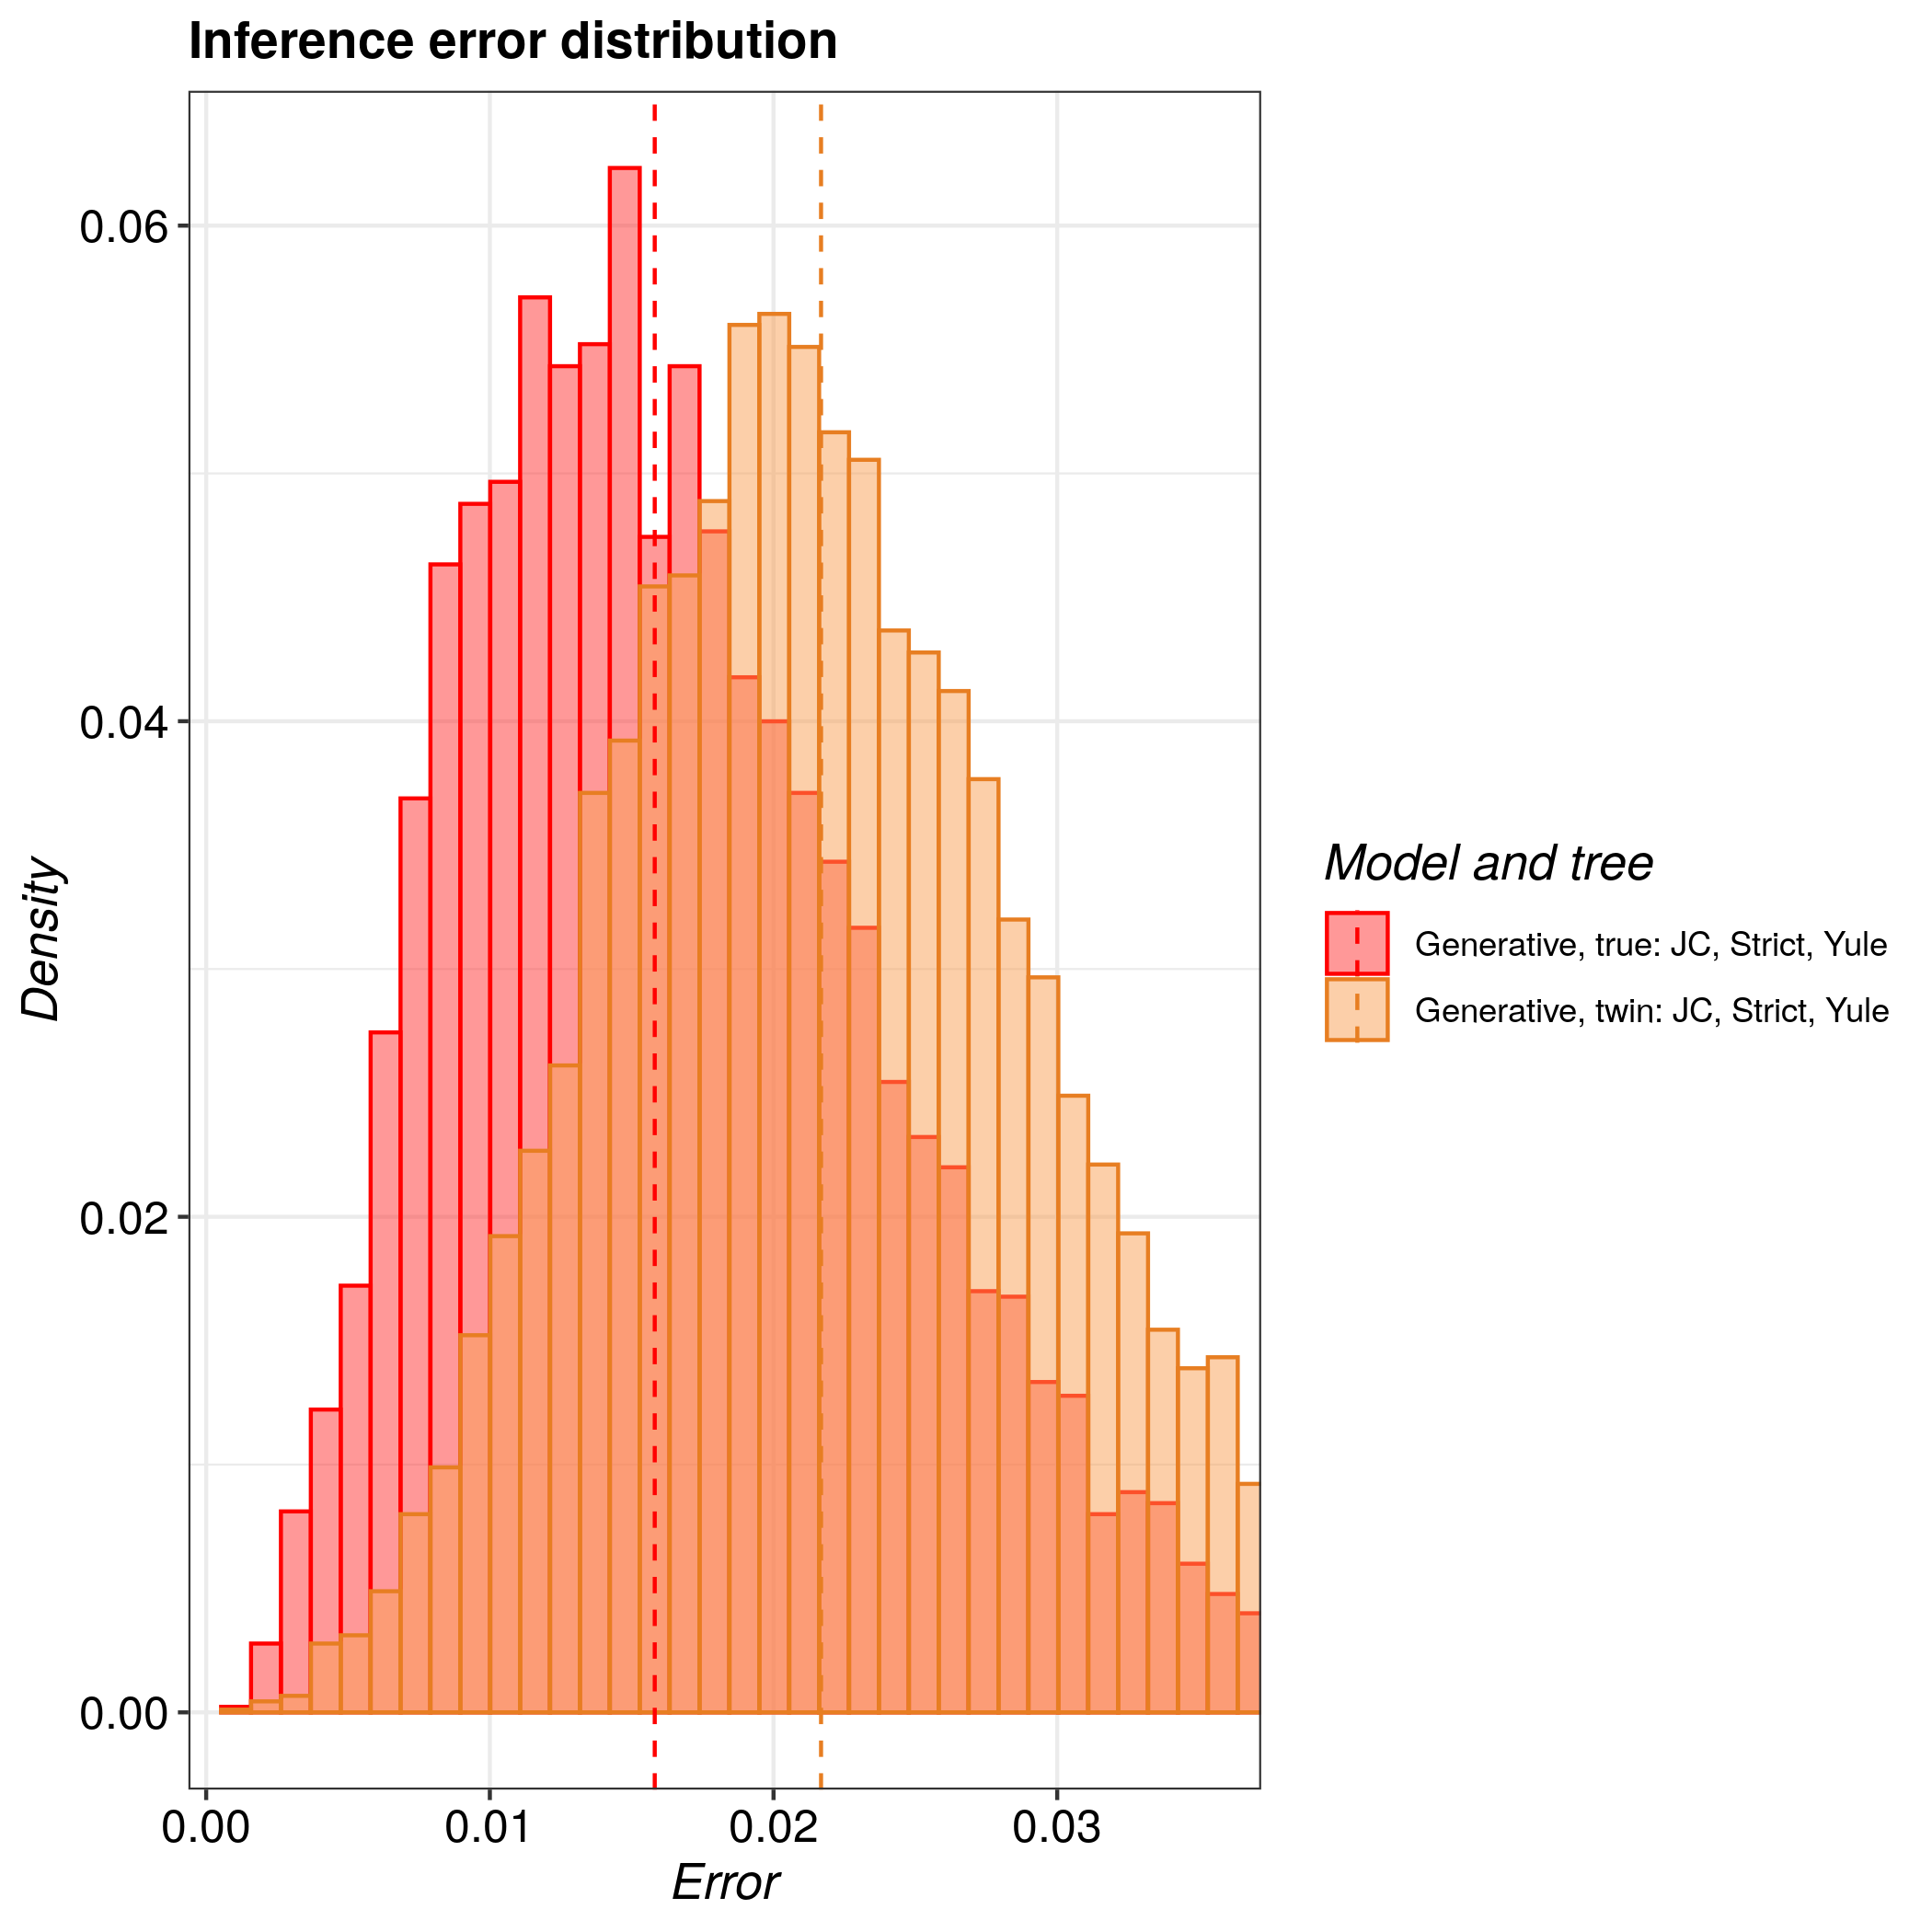
\includegraphics[width=\textwidth]{pirouette_example_21/example_21_319/errors.png}
  \caption{4000 nucleotides}
\end{figure}

\begin{figure}[H]
  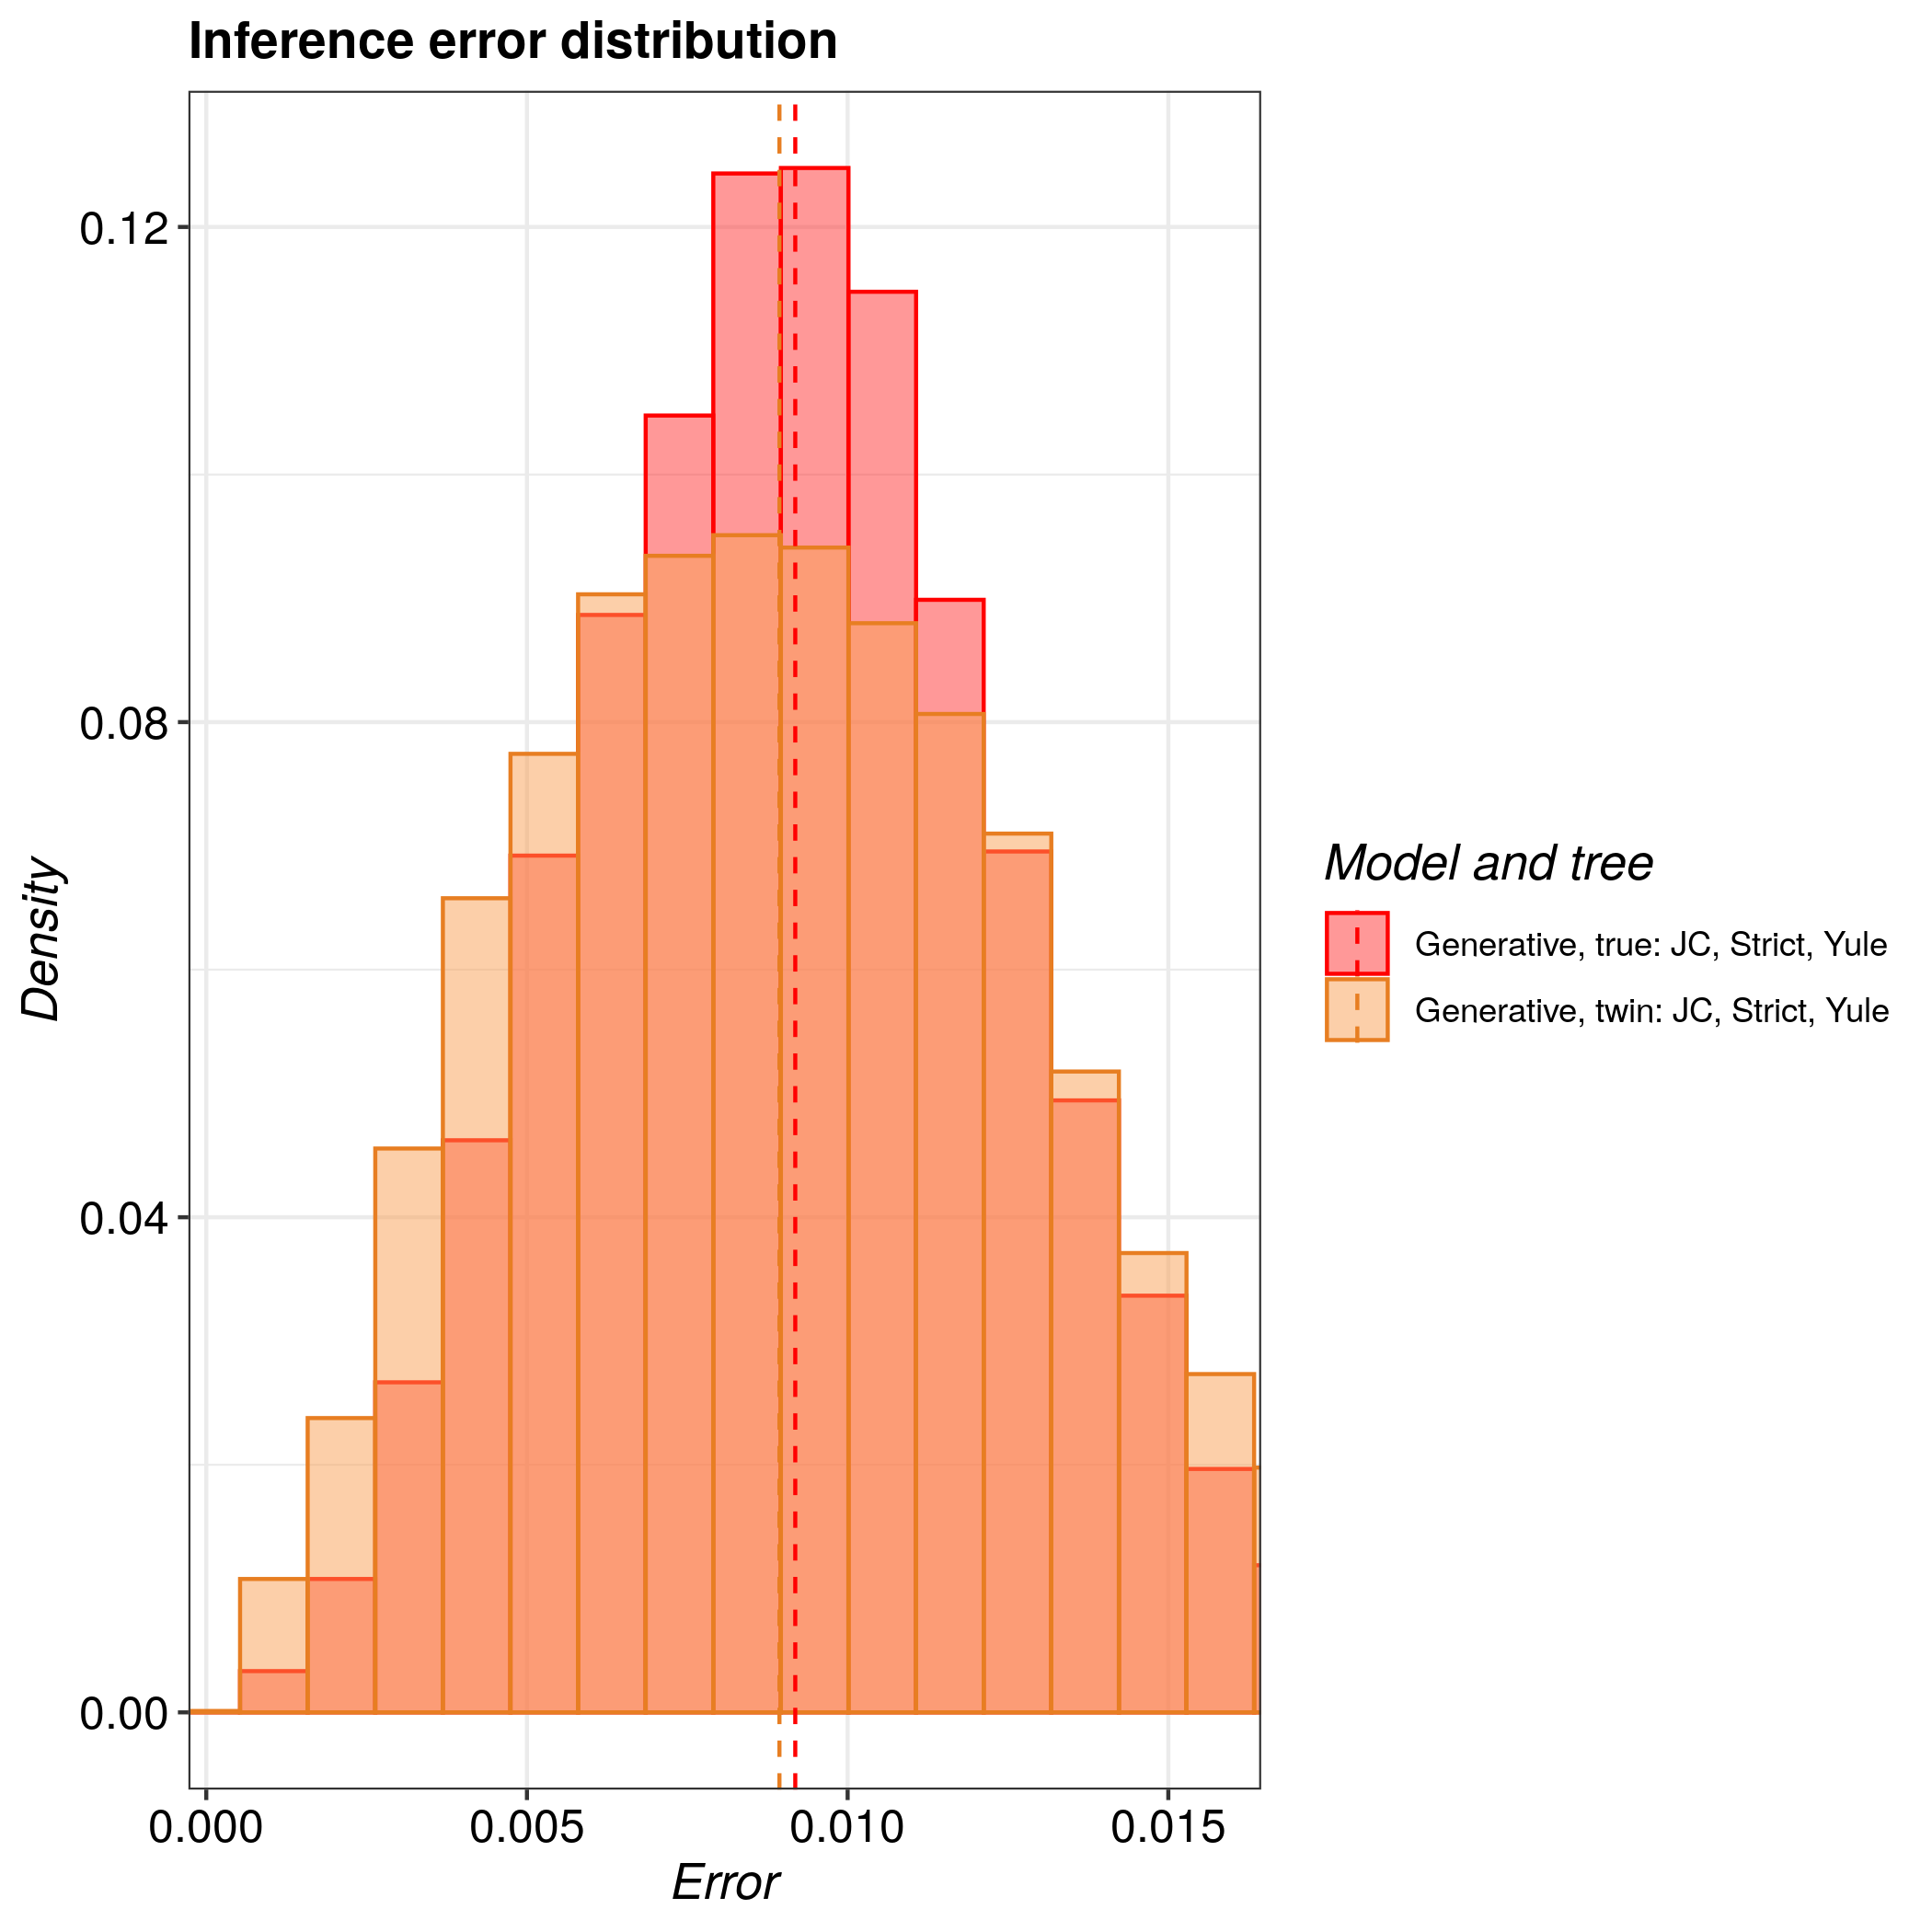
\includegraphics[width=\textwidth]{pirouette_example_21/example_21_320/errors.png}
  \caption{8000 nucleotides}
\end{figure}

\begin{figure}[H]
  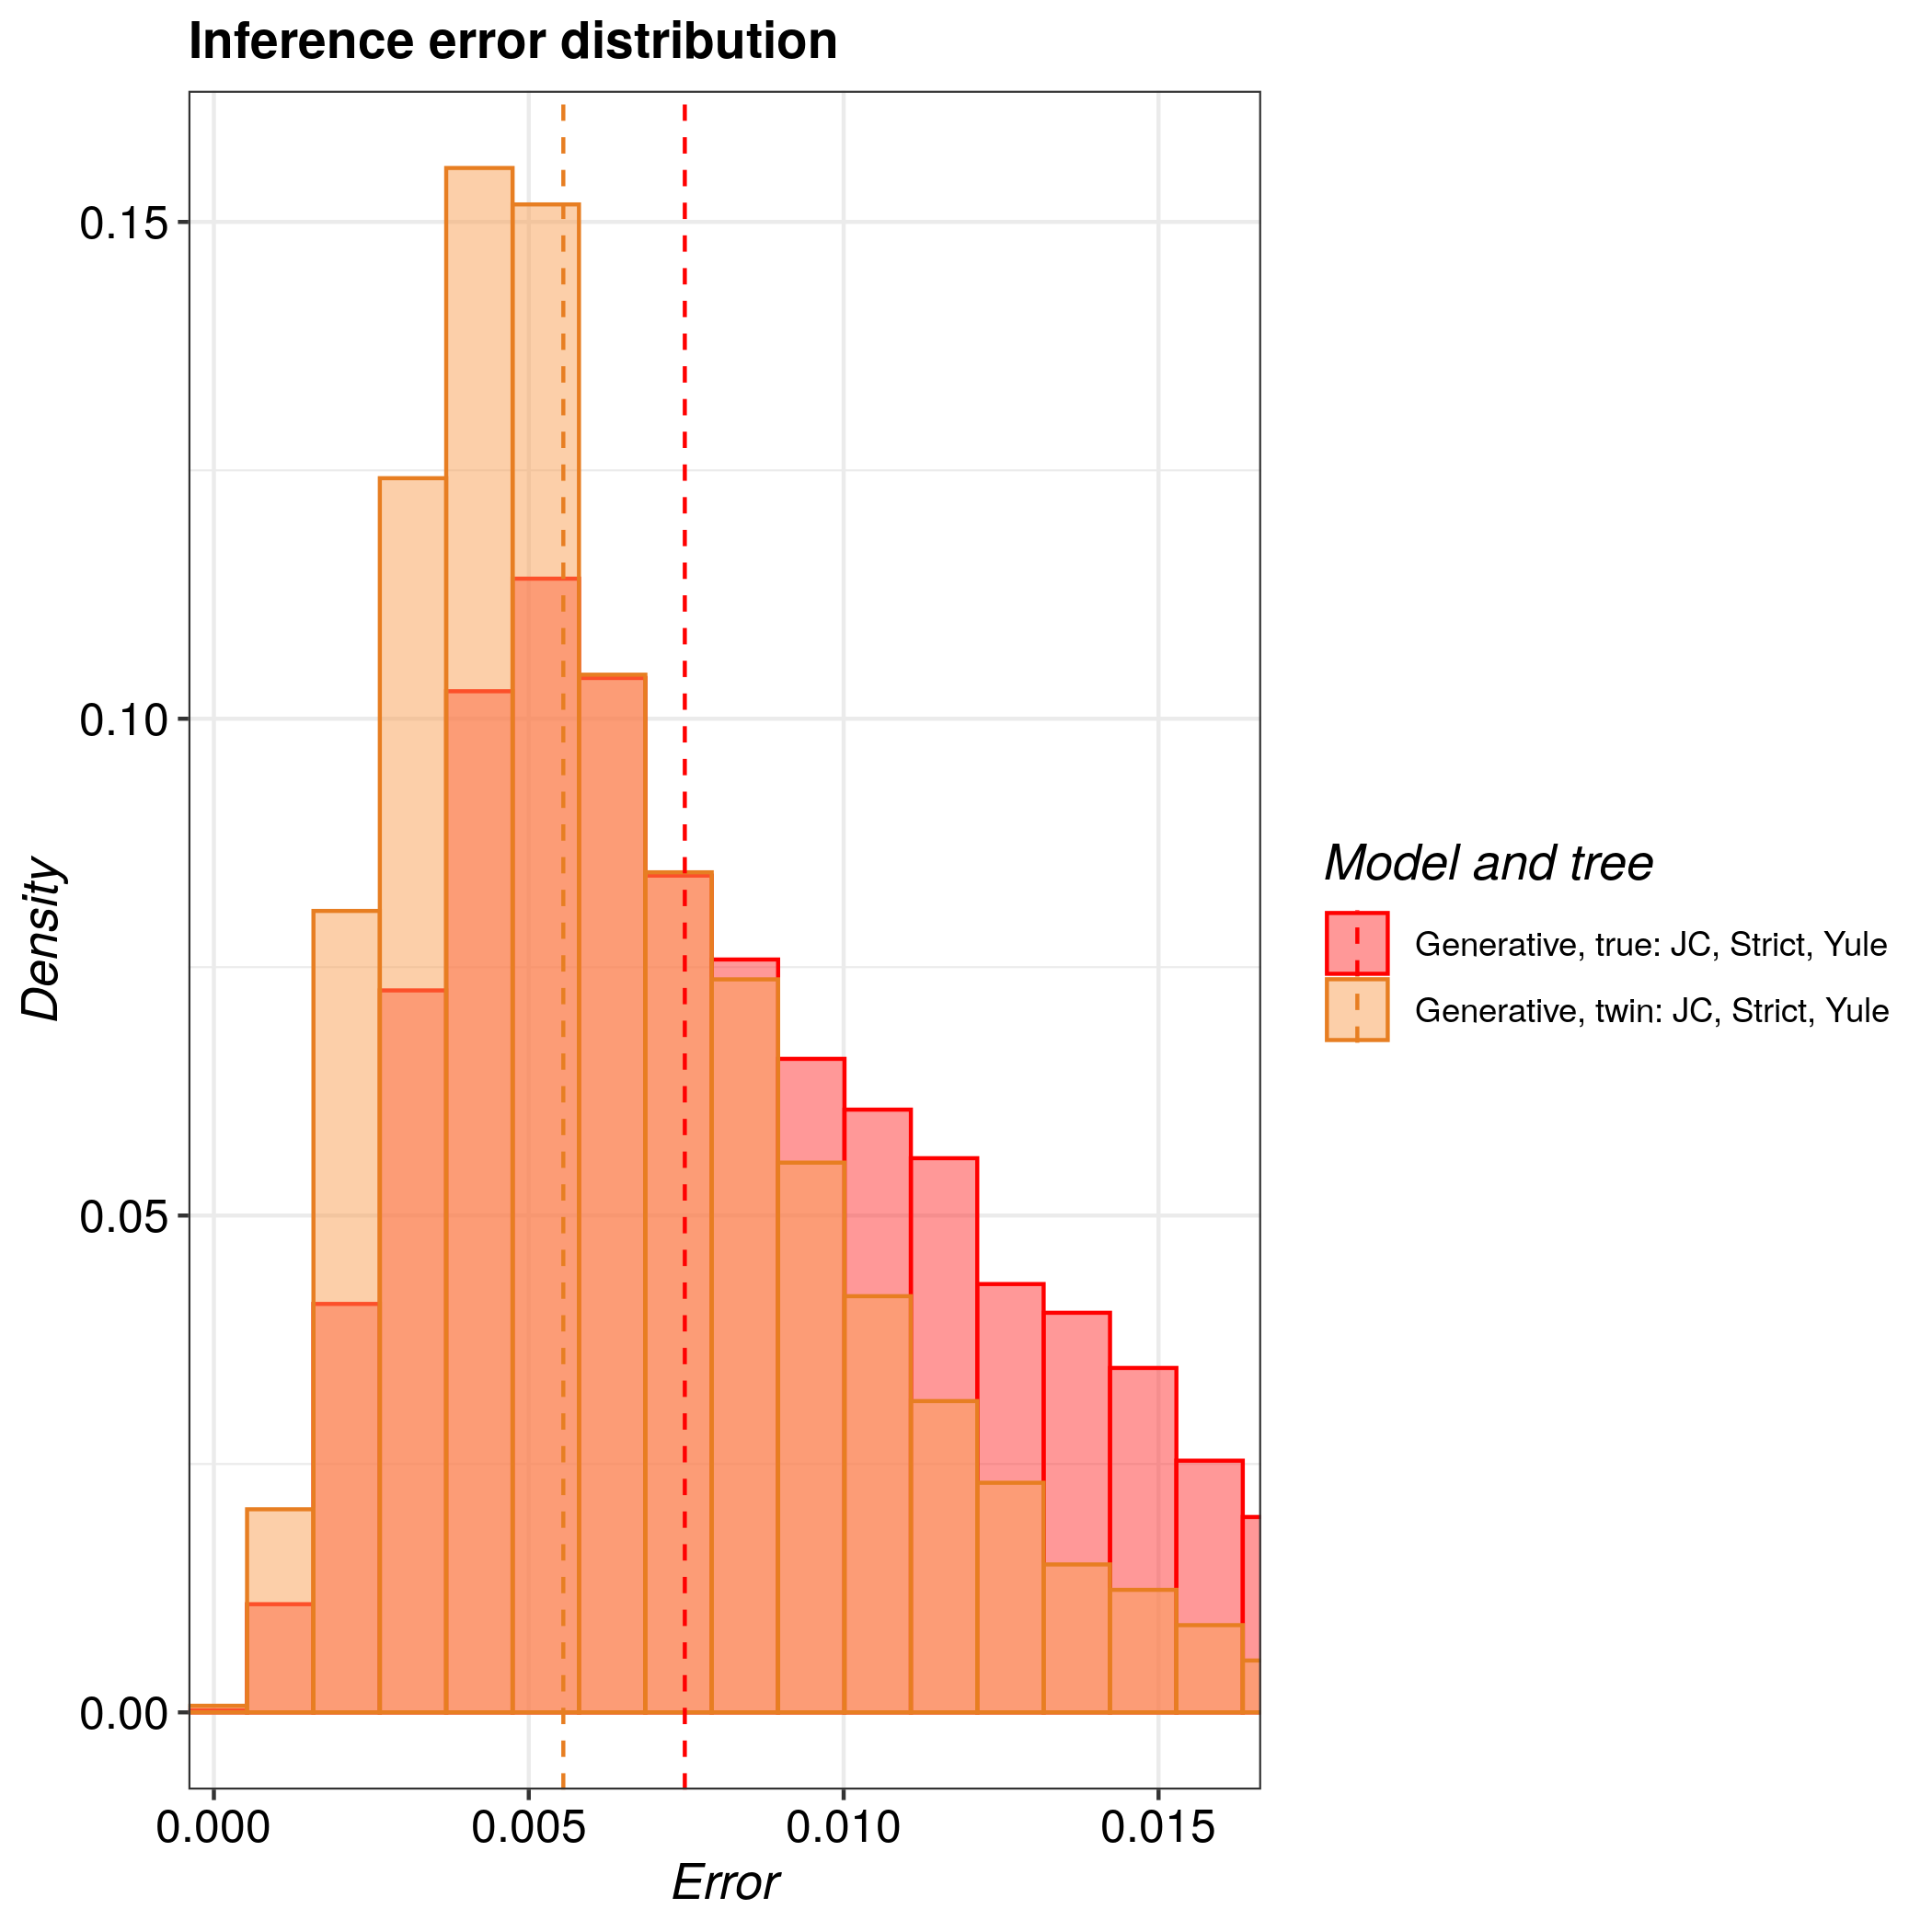
\includegraphics[width=\textwidth]{pirouette_example_21/example_21_321/errors.png}
  \caption{16000 nucleotides}
\end{figure}

%%%%%%%%%%%%%%%%%%%%%%%%%%%%%%%%%%%%%%%%%%%%%%%%%%%%%%%%%%%%%%%%%%%%%%%%%%%%%%%%
\subsection{The effect of non-clock like models}
%%%%%%%%%%%%%%%%%%%%%%%%%%%%%%%%%%%%%%%%%%%%%%%%%%%%%%%%%%%%%%%%%%%%%%%%%%%%%%%%

The code used in this part of the article can be found at 
\url{https://github.com/richelbilderbeek/pirouette_example_17}.

\begin{figure}[H]
  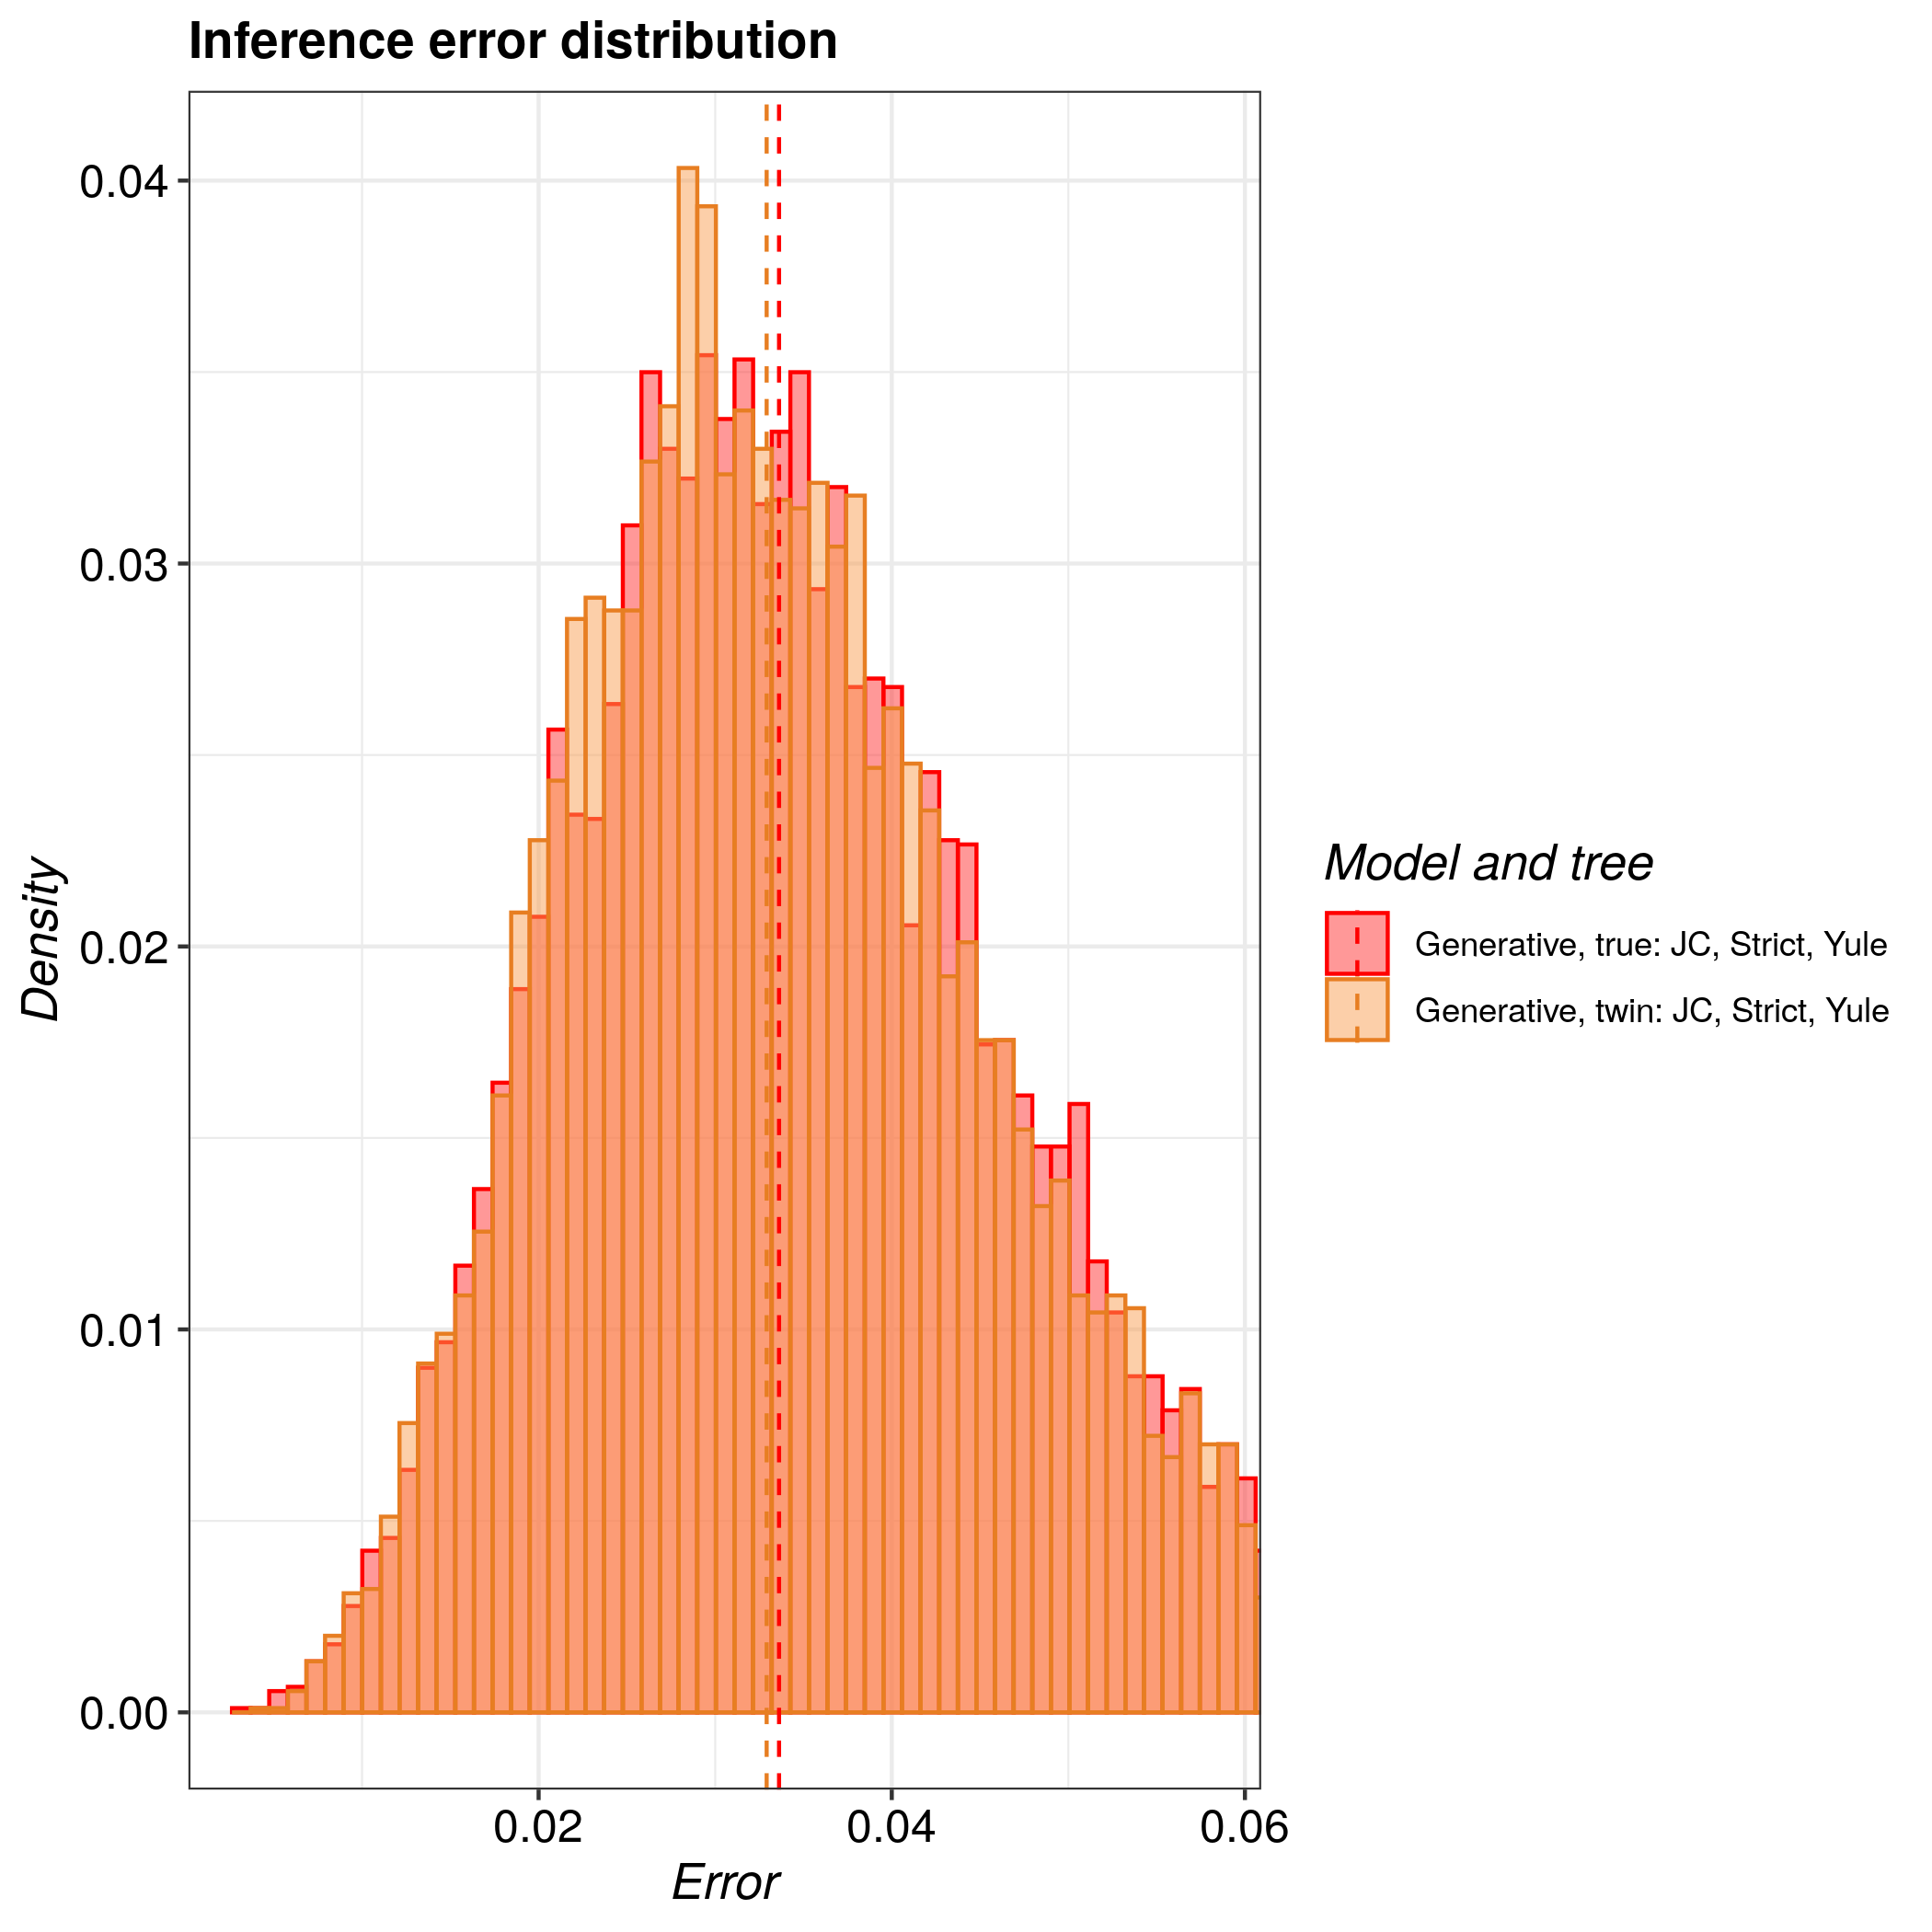
\includegraphics[width=\textwidth]{pirouette_example_17/example_17_314/errors.png}
  \caption{An unliked node substitution model}
\end{figure}

%%%%%%%%%%%%%%%%%%%%%%%%%%%%%%%%%%%%%%%%%%%%%%%%%%%%%%%%%%%%%%%%%%%%%%%%%%%%%%%%
\subsection{The effect of assuming a Yule tree prior on a Yule tree}
%%%%%%%%%%%%%%%%%%%%%%%%%%%%%%%%%%%%%%%%%%%%%%%%%%%%%%%%%%%%%%%%%%%%%%%%%%%%%%%%

The code used in this part of the article can be found at 
\url{https://github.com/richelbilderbeek/pirouette_example_22}.

\begin{figure}[H]
  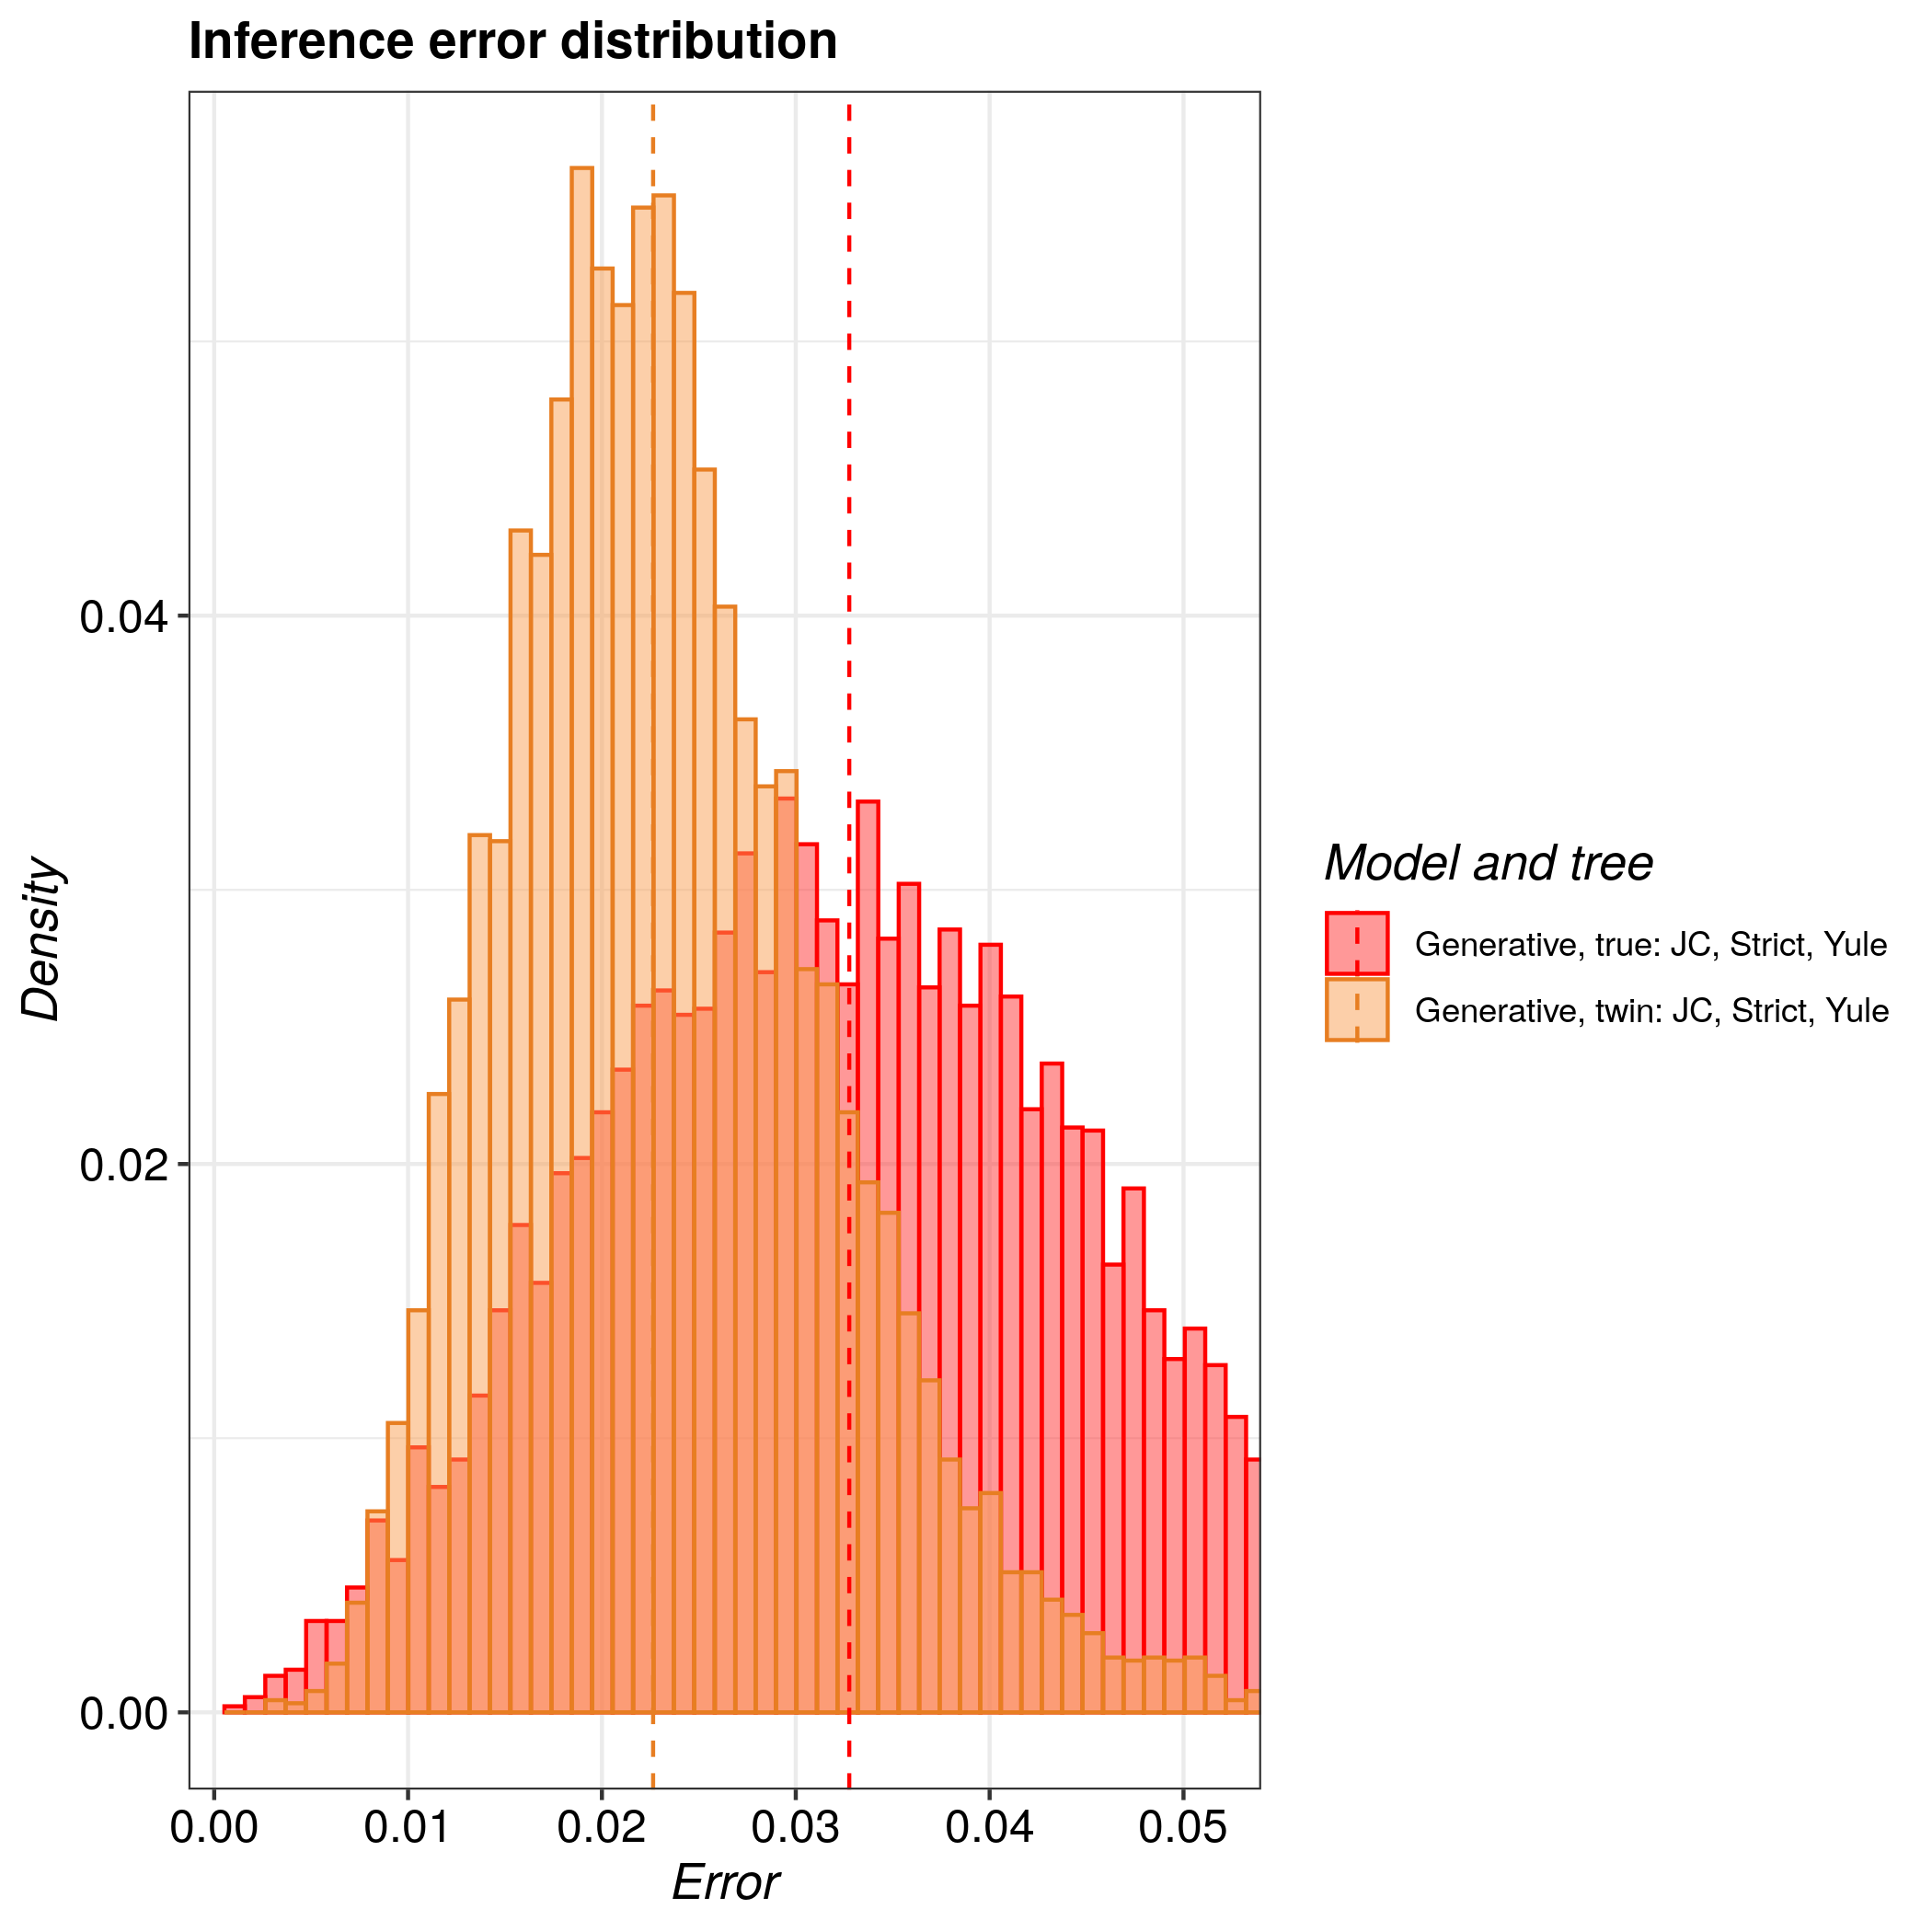
\includegraphics[width=\textwidth]{pirouette_example_22/example_22_314/errors.png}
  \caption{Assuming a Yule tree prior on a Yule tree}
\end{figure}

%%%%%%%%%%%%%%%%%%%%%%%%%%%%%%%%%%%%%%%%%%%%%%%%%%%%%%%%%%%%%%%%%%%%%%%%%%%%%%%%
\subsection{The effect of assuming a Yule tree prior on a BD tree}
%%%%%%%%%%%%%%%%%%%%%%%%%%%%%%%%%%%%%%%%%%%%%%%%%%%%%%%%%%%%%%%%%%%%%%%%%%%%%%%%

The code used in this part of the article can be found at 
\url{https://github.com/richelbilderbeek/pirouette_example_26}.

\begin{figure}[H]
  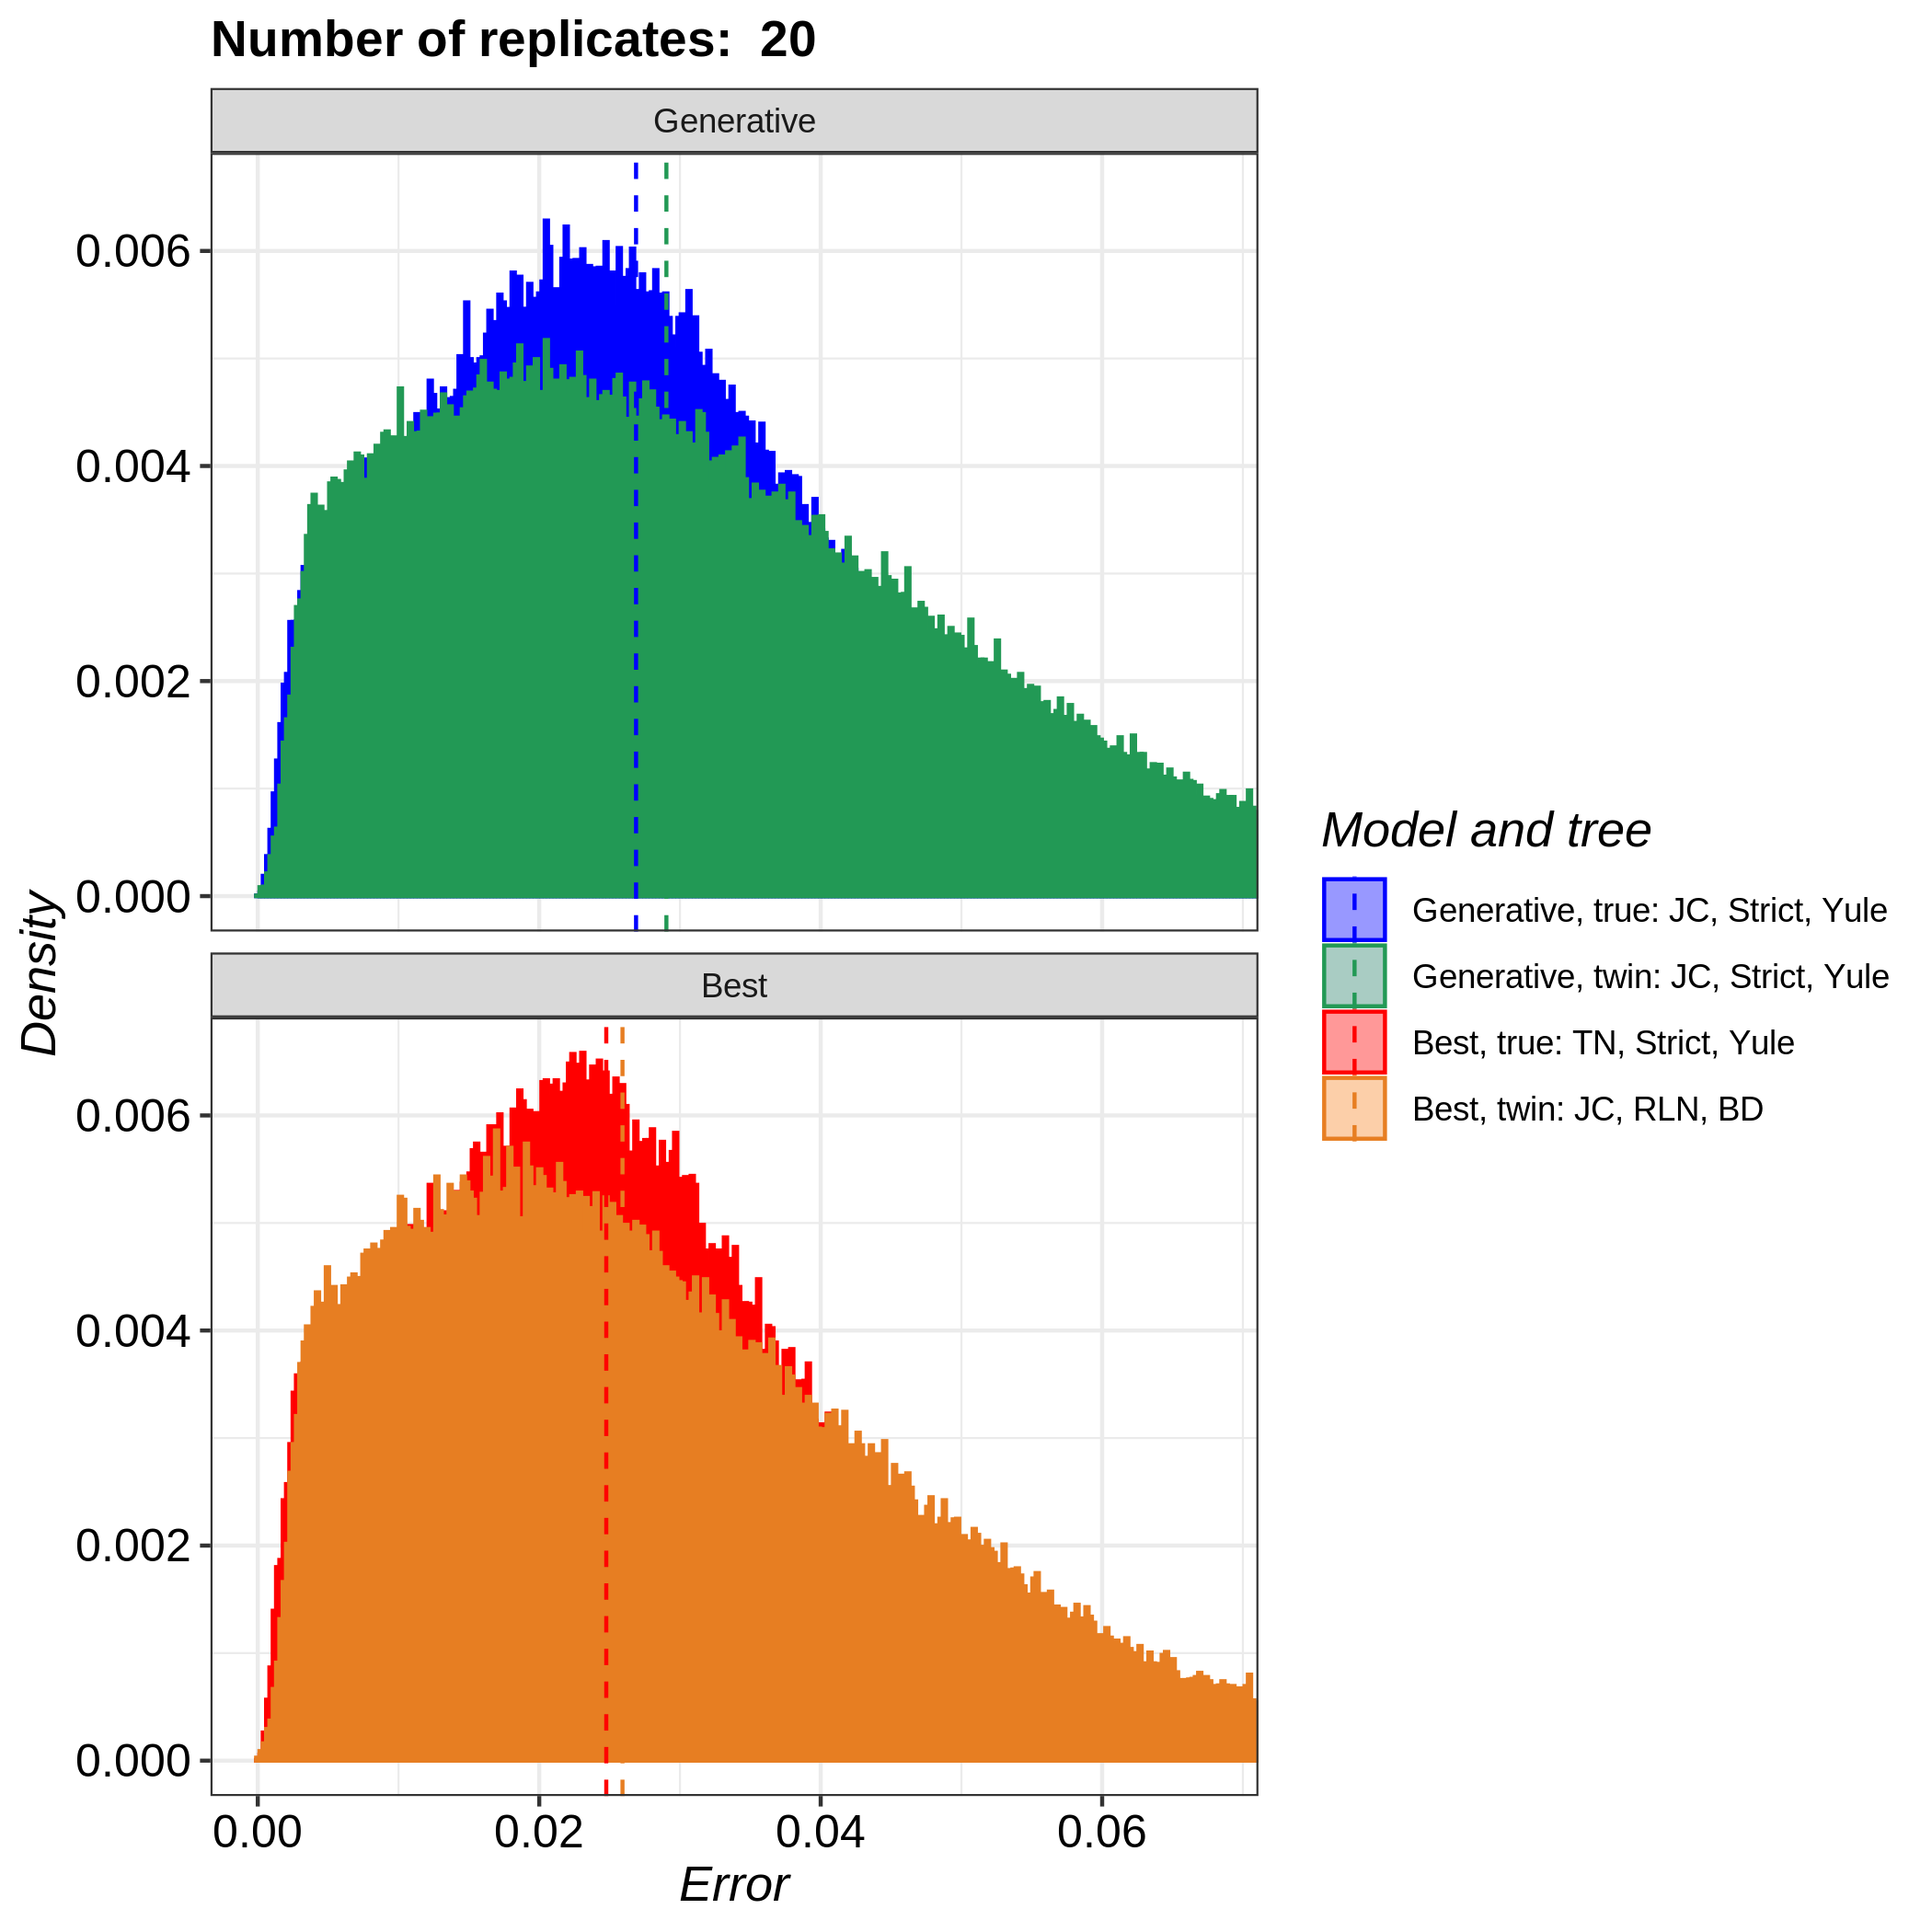
\includegraphics[width=\textwidth]{pirouette_example_26/example_26_314/errors.png}
  \caption{Assuming a Yule tree prior on a BD tree}
\end{figure}

%%%%%%%%%%%%%%%%%%%%%%%%%%%%%%%%%%%%%%%%%%%%%%%%%%%%%%%%%%%%%%%%%%%%%%%%%%%%%%%%
\subsection{The effect of differently common diversity-dependent trees}
%%%%%%%%%%%%%%%%%%%%%%%%%%%%%%%%%%%%%%%%%%%%%%%%%%%%%%%%%%%%%%%%%%%%%%%%%%%%%%%%

The code used in this part of the article can be found at 
\url{https://github.com/richelbilderbeek/pirouette_example_23}.

\begin{figure}[H]
  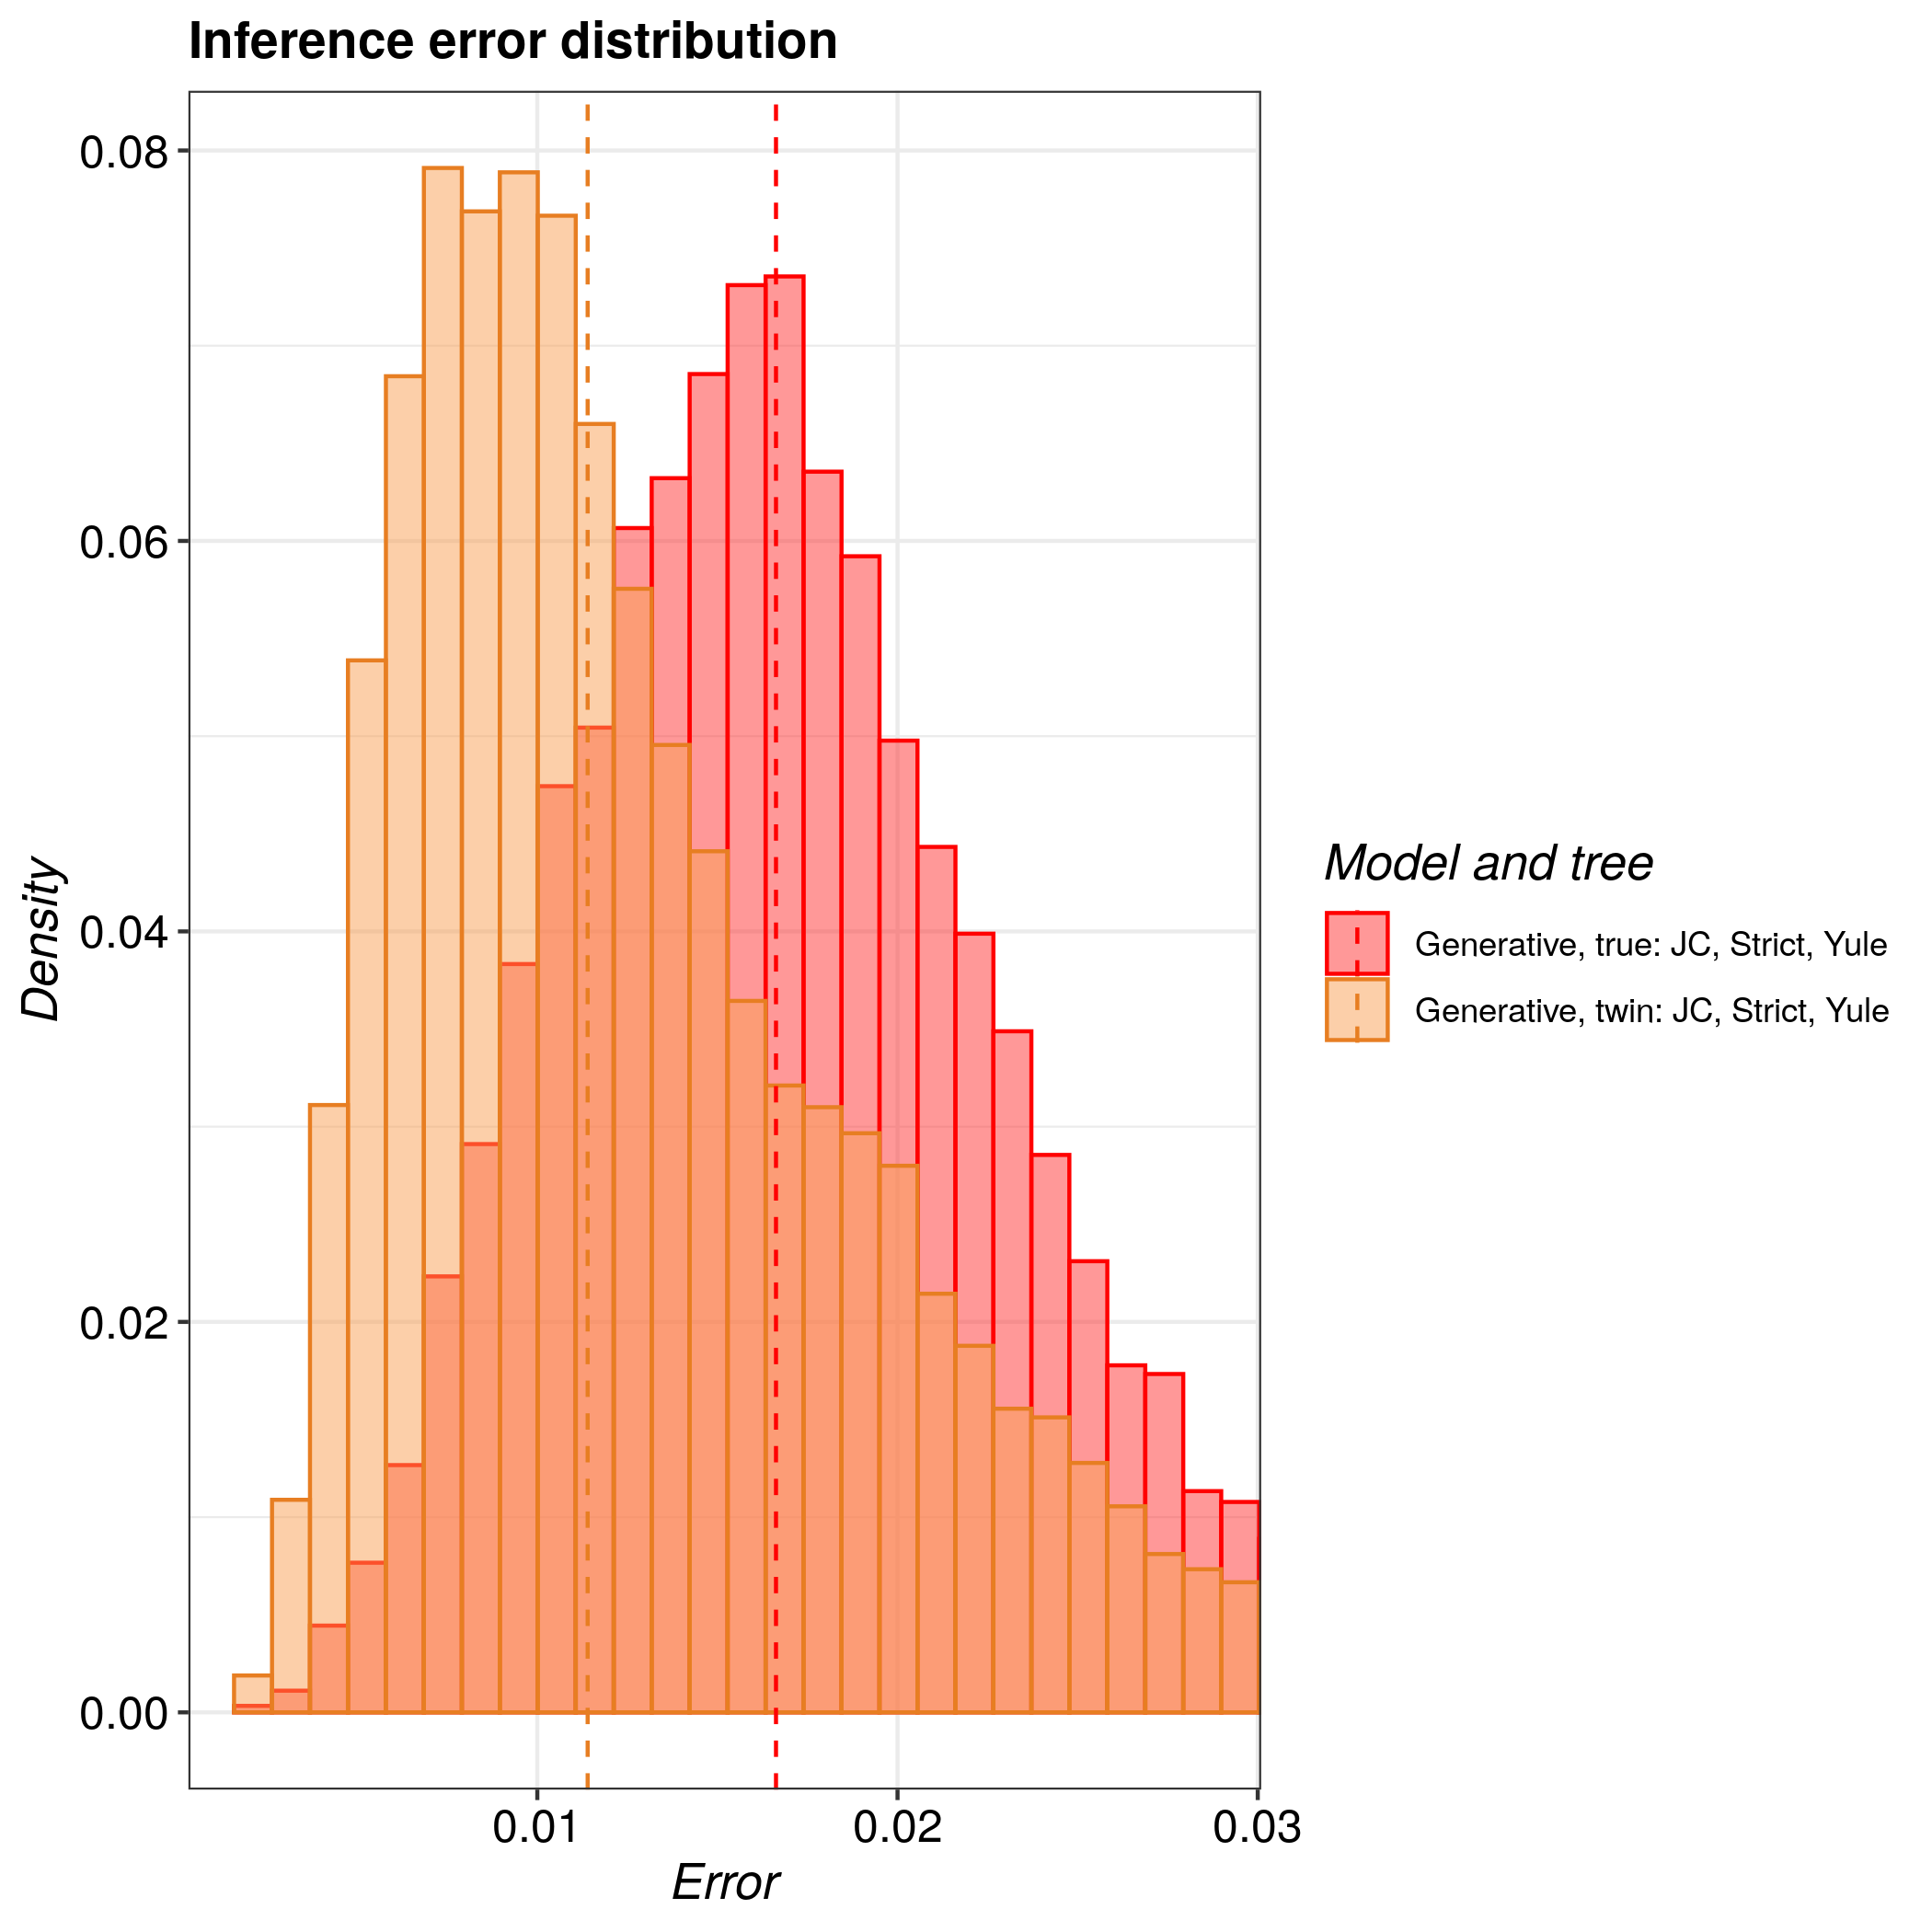
\includegraphics[width=\textwidth]{pirouette_example_23/example_23_314/errors.png}
  \caption{Lowest likelihood}
\end{figure}

\begin{figure}[H]
  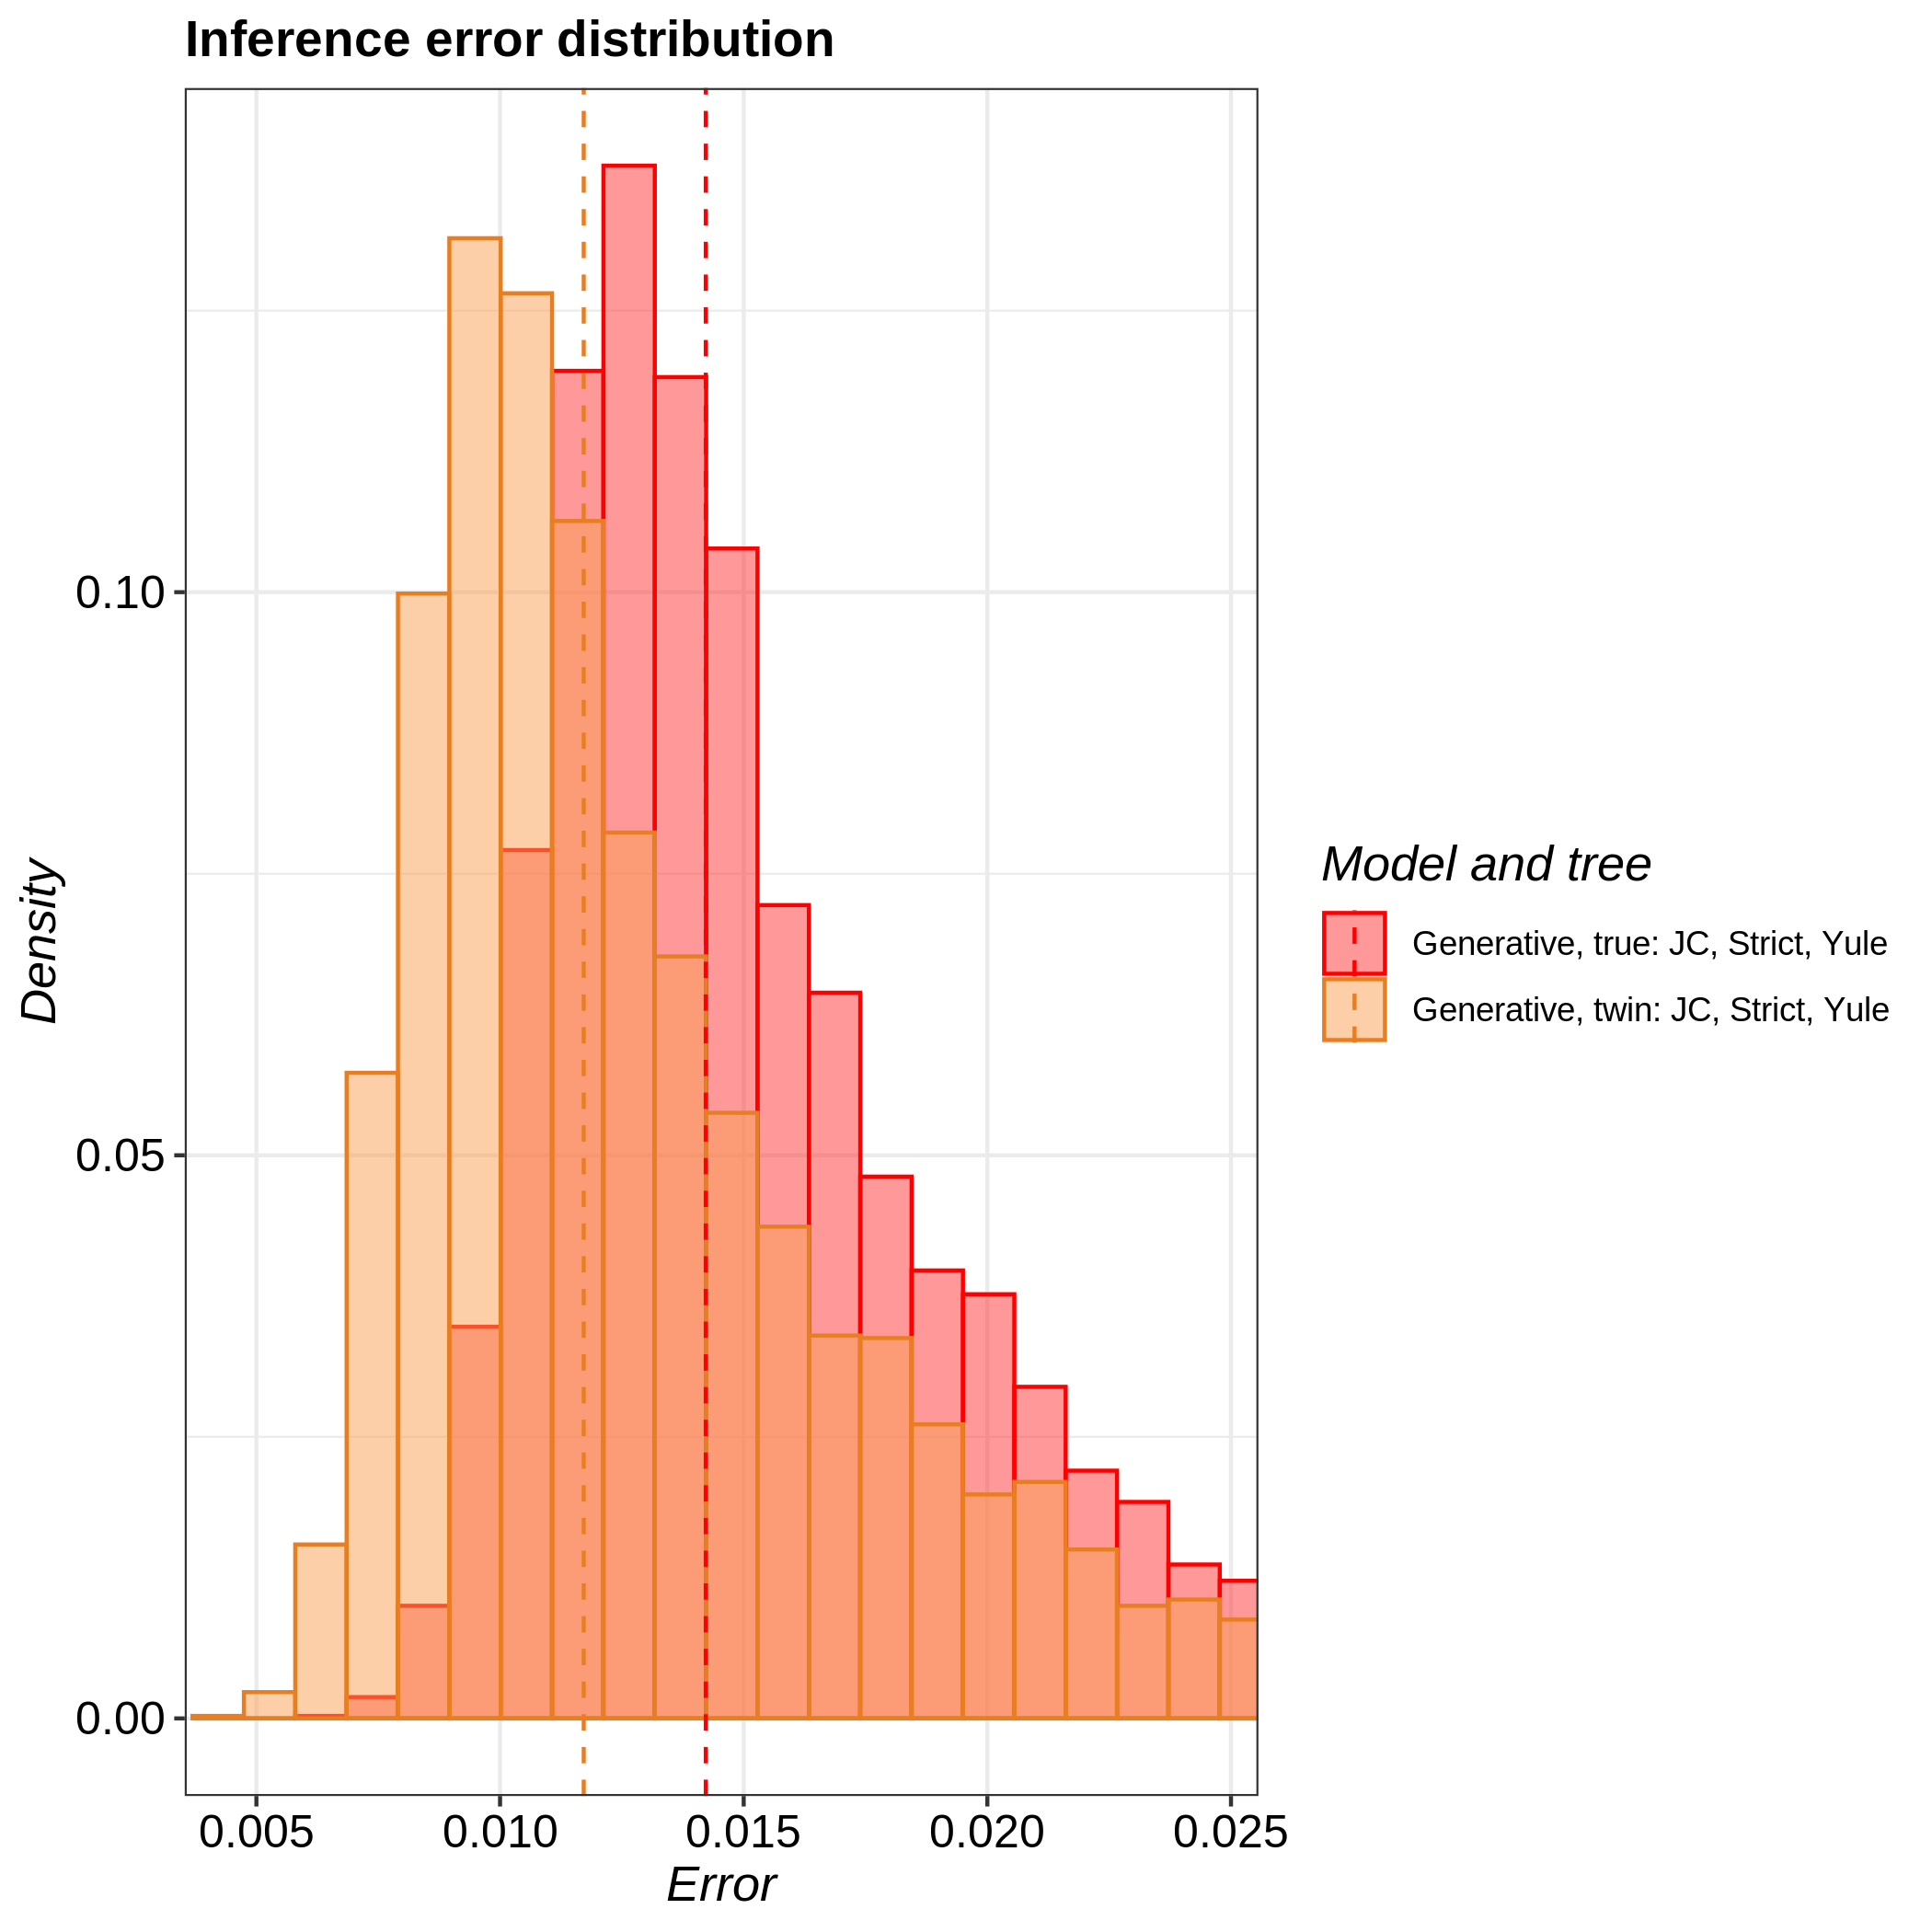
\includegraphics[width=\textwidth]{pirouette_example_23/example_23_315/errors.png}
  \caption{Between lowest and median likelihood}
\end{figure}

\begin{figure}[H]
  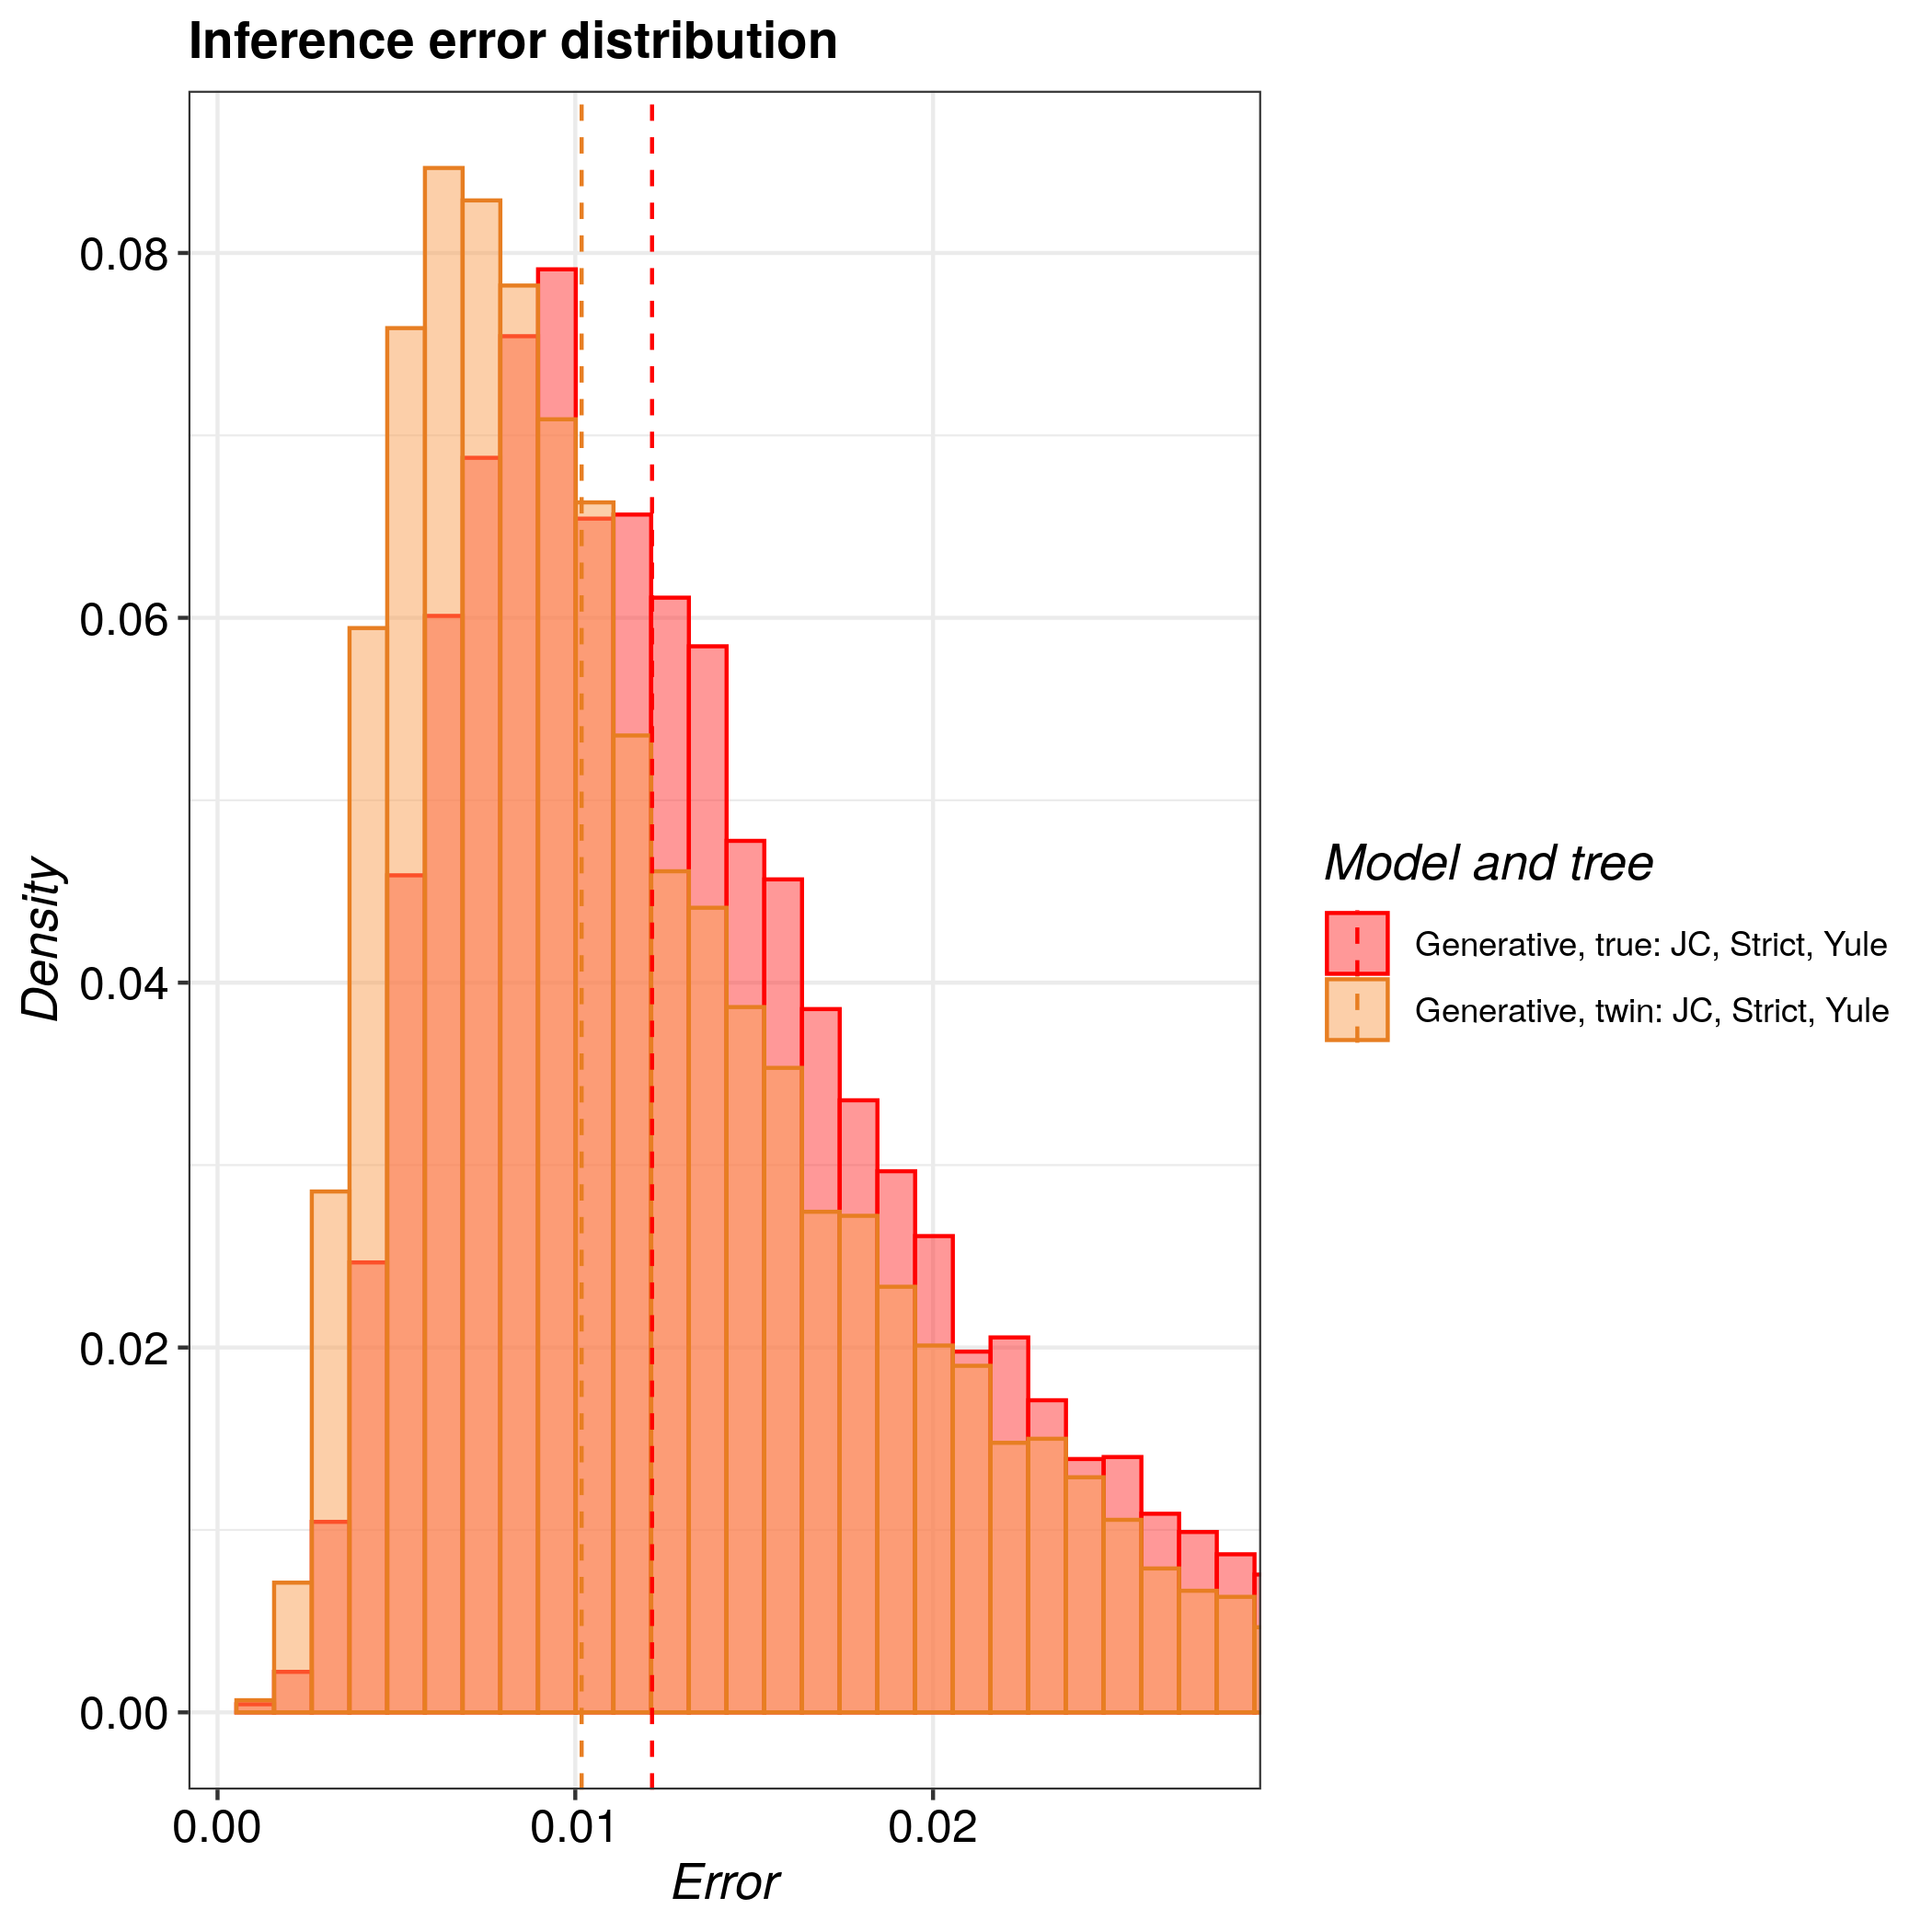
\includegraphics[width=\textwidth]{pirouette_example_23/example_23_316/errors.png}
  \caption{Median likelihood}
\end{figure}


\begin{figure}[H]
  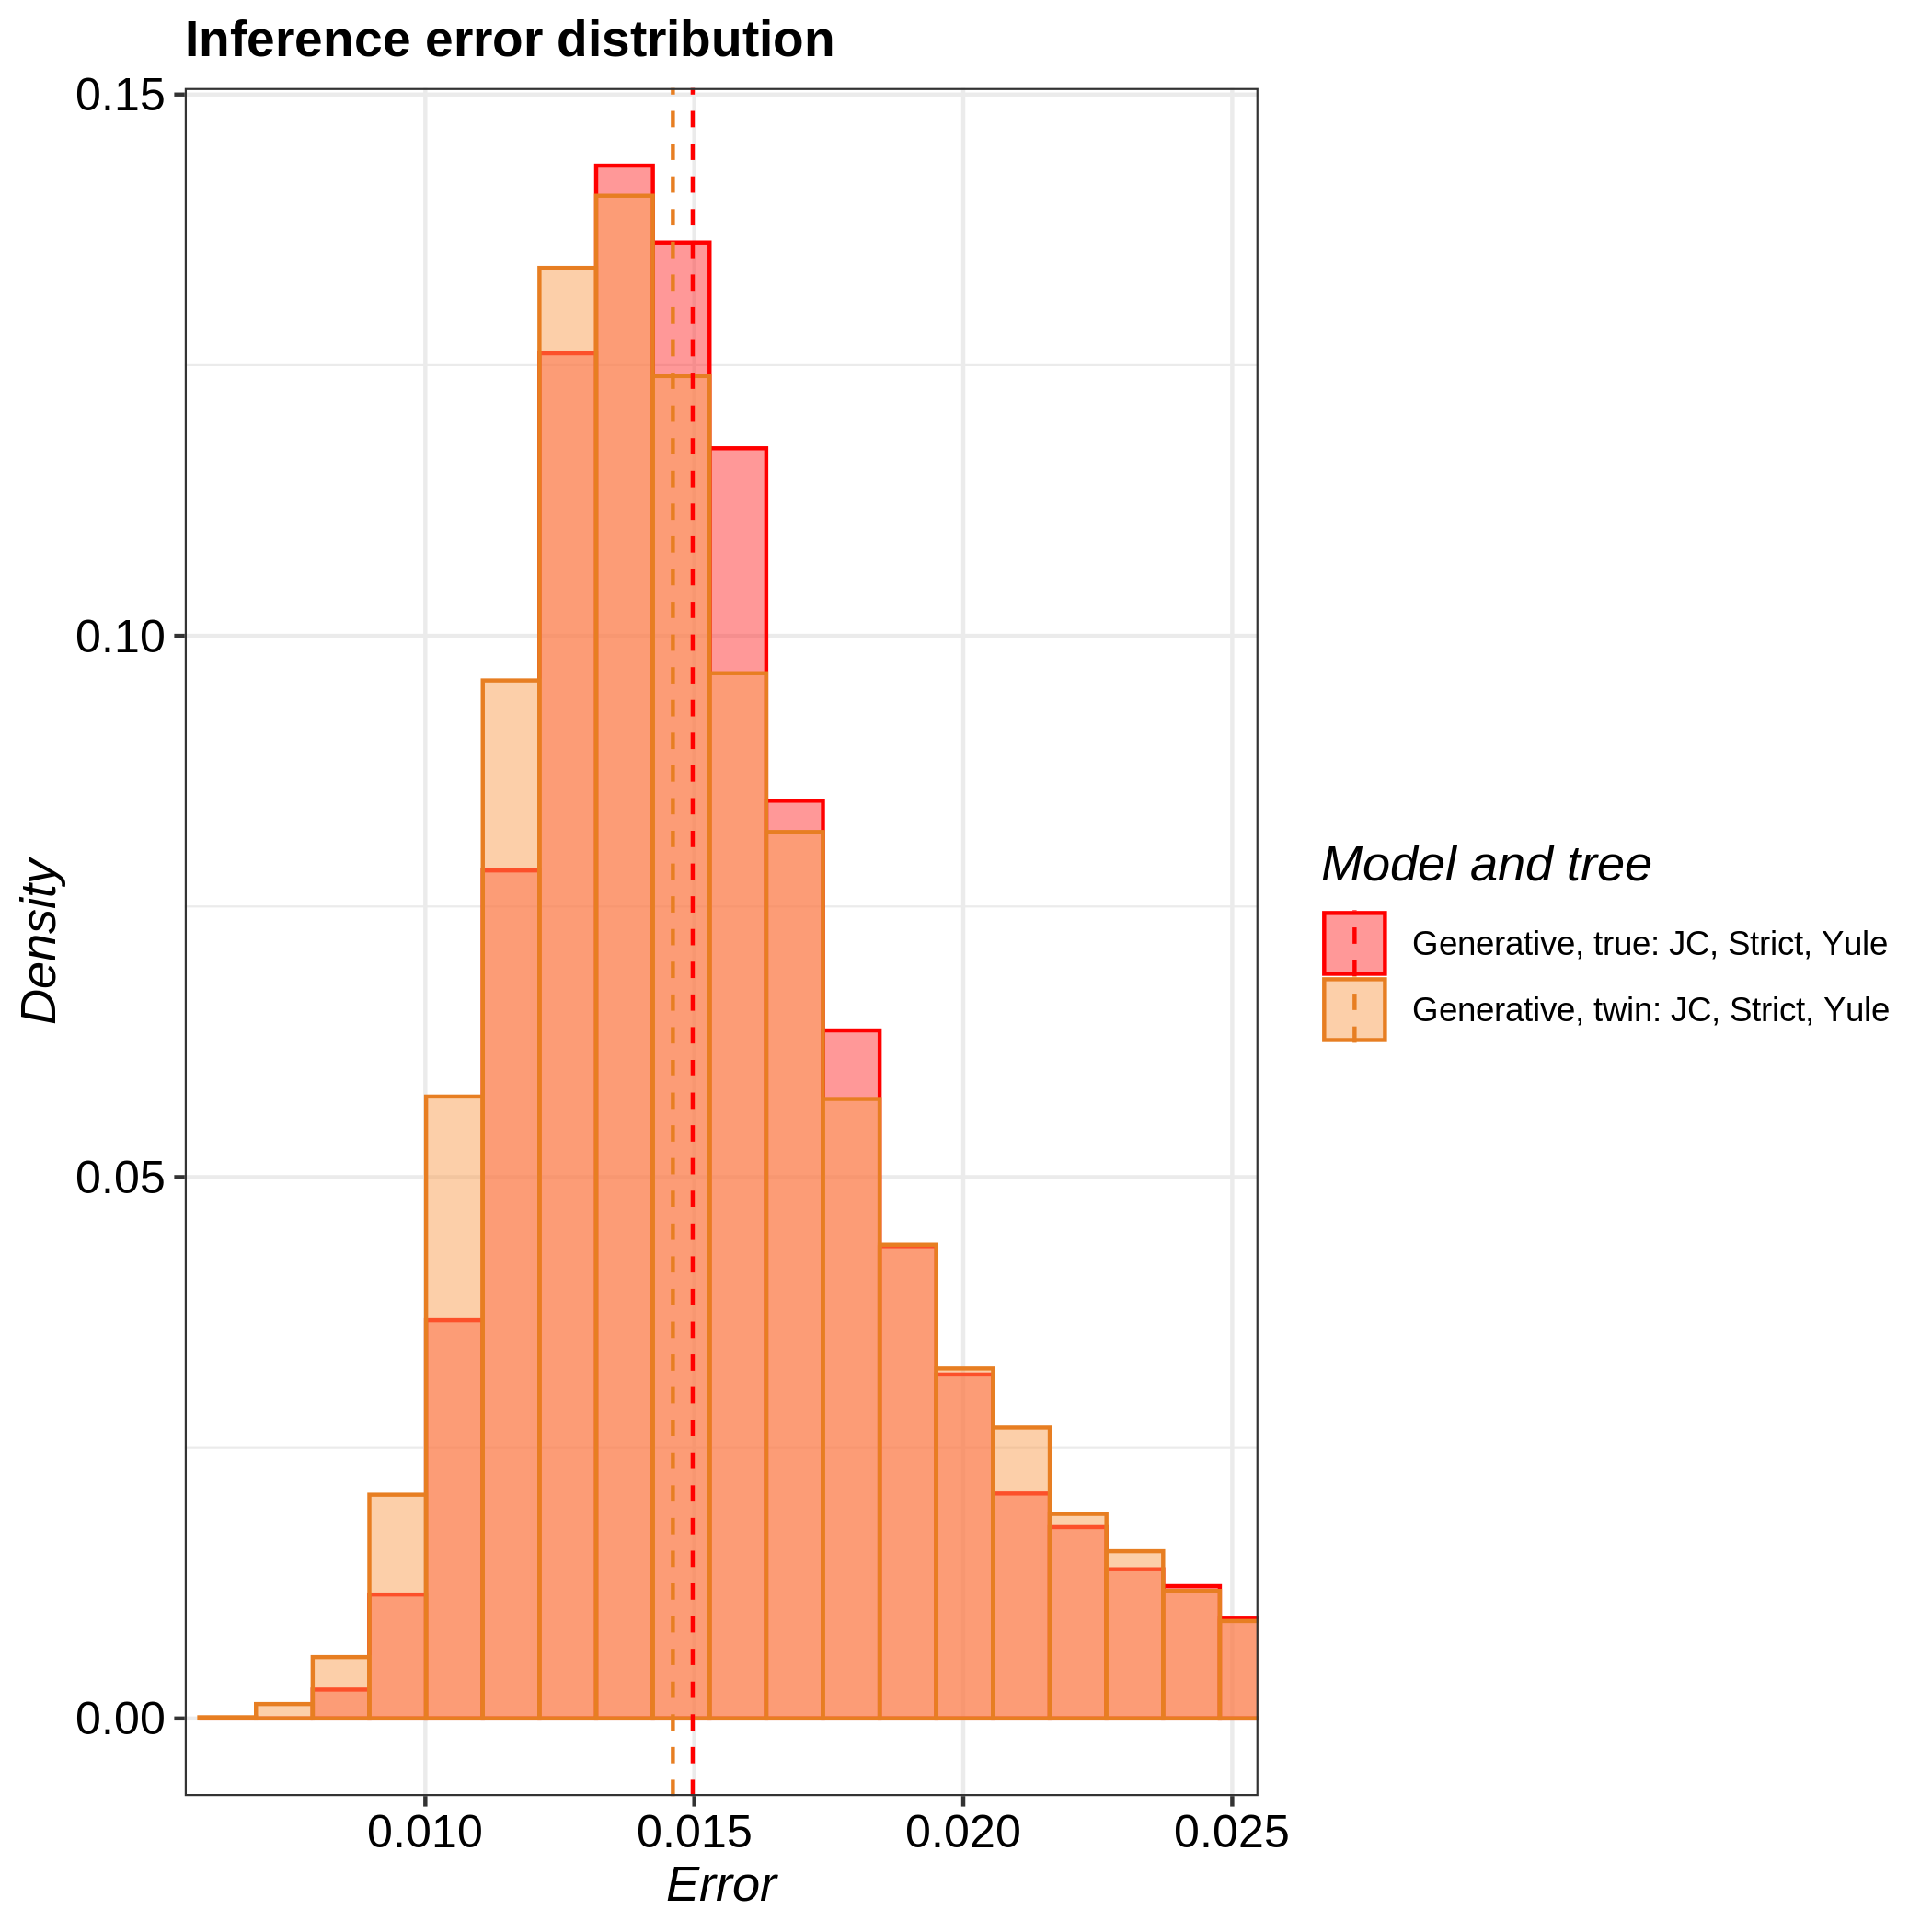
\includegraphics[width=\textwidth]{pirouette_example_23/example_23_317/errors.png}
  \caption{Between median and highest likelihood}
\end{figure}

\begin{figure}[H]
  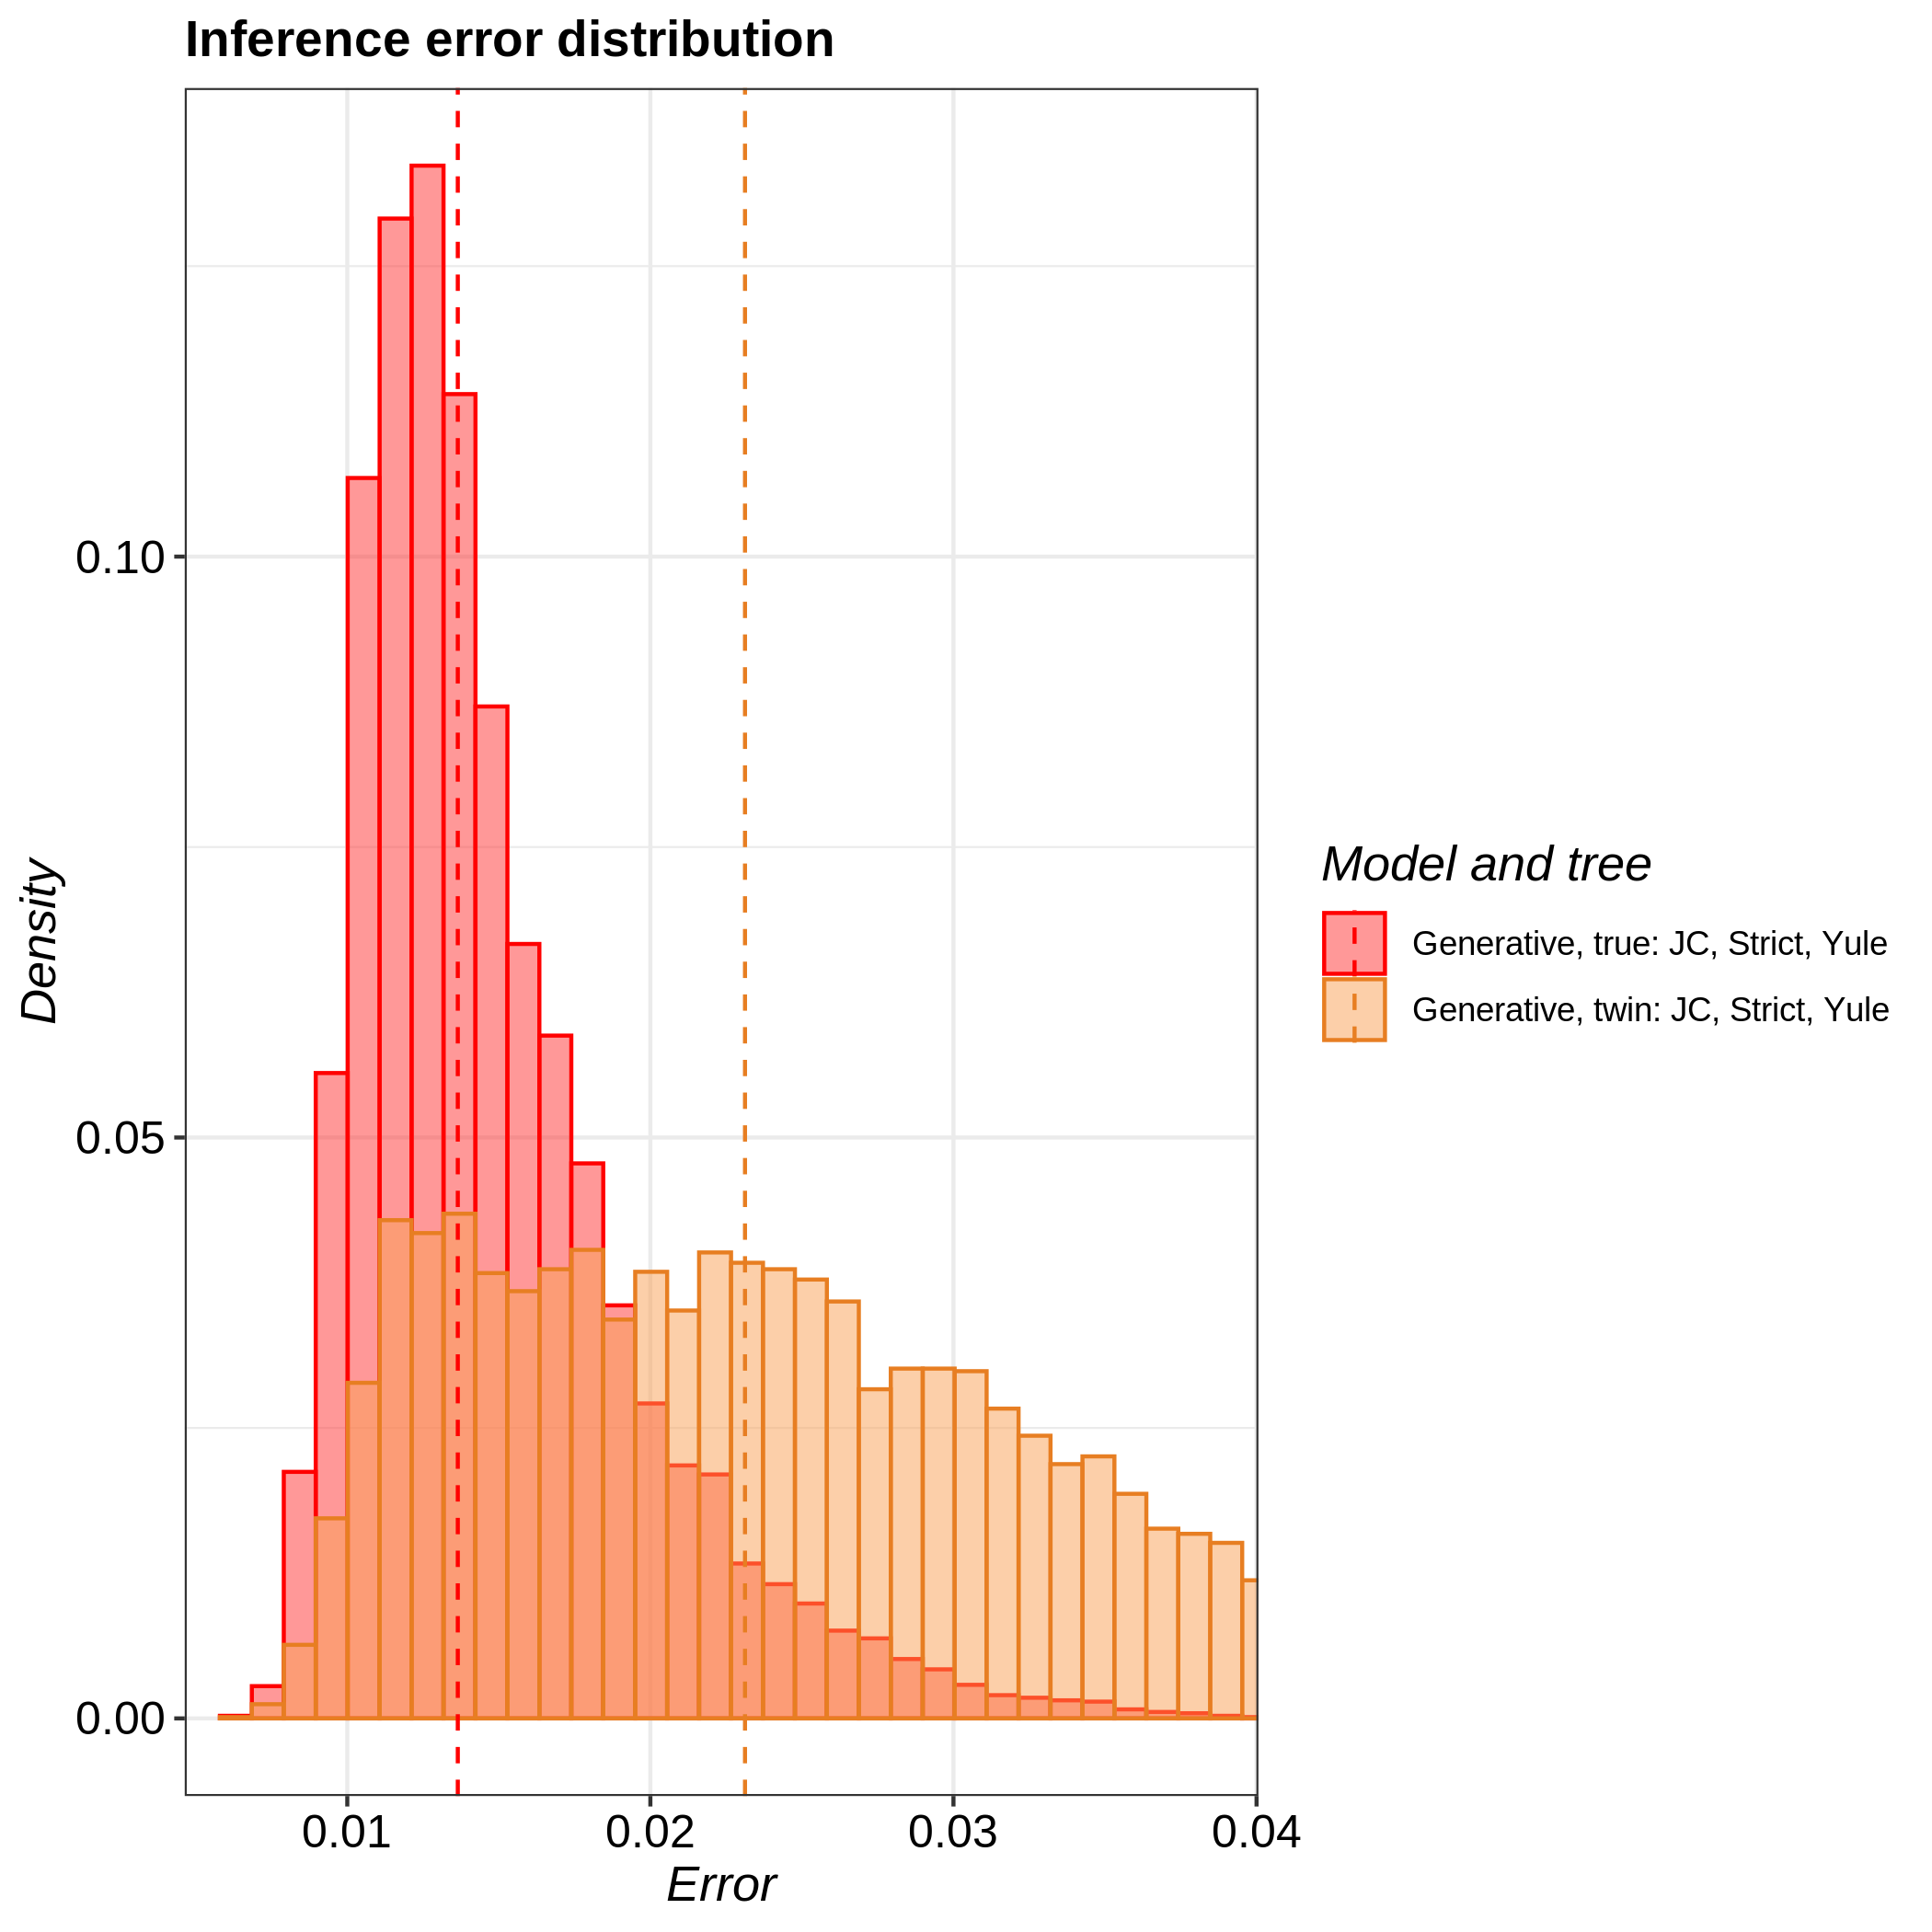
\includegraphics[width=\textwidth]{pirouette_example_23/example_23_318/errors.png}
  \caption{Highest likelihood}
\end{figure}

%%%%%%%%%%%%%%%%%%%%%%%%%%%%%%%%%%%%%%%%%%%%%%%%%%%%%%%%%%%%%%%%%%%%%%%%%%%%%%%%
\subsection{The effect of equal or equalized mutation rate in the twin alignment}
%%%%%%%%%%%%%%%%%%%%%%%%%%%%%%%%%%%%%%%%%%%%%%%%%%%%%%%%%%%%%%%%%%%%%%%%%%%%%%%%

\begin{figure}[H]
  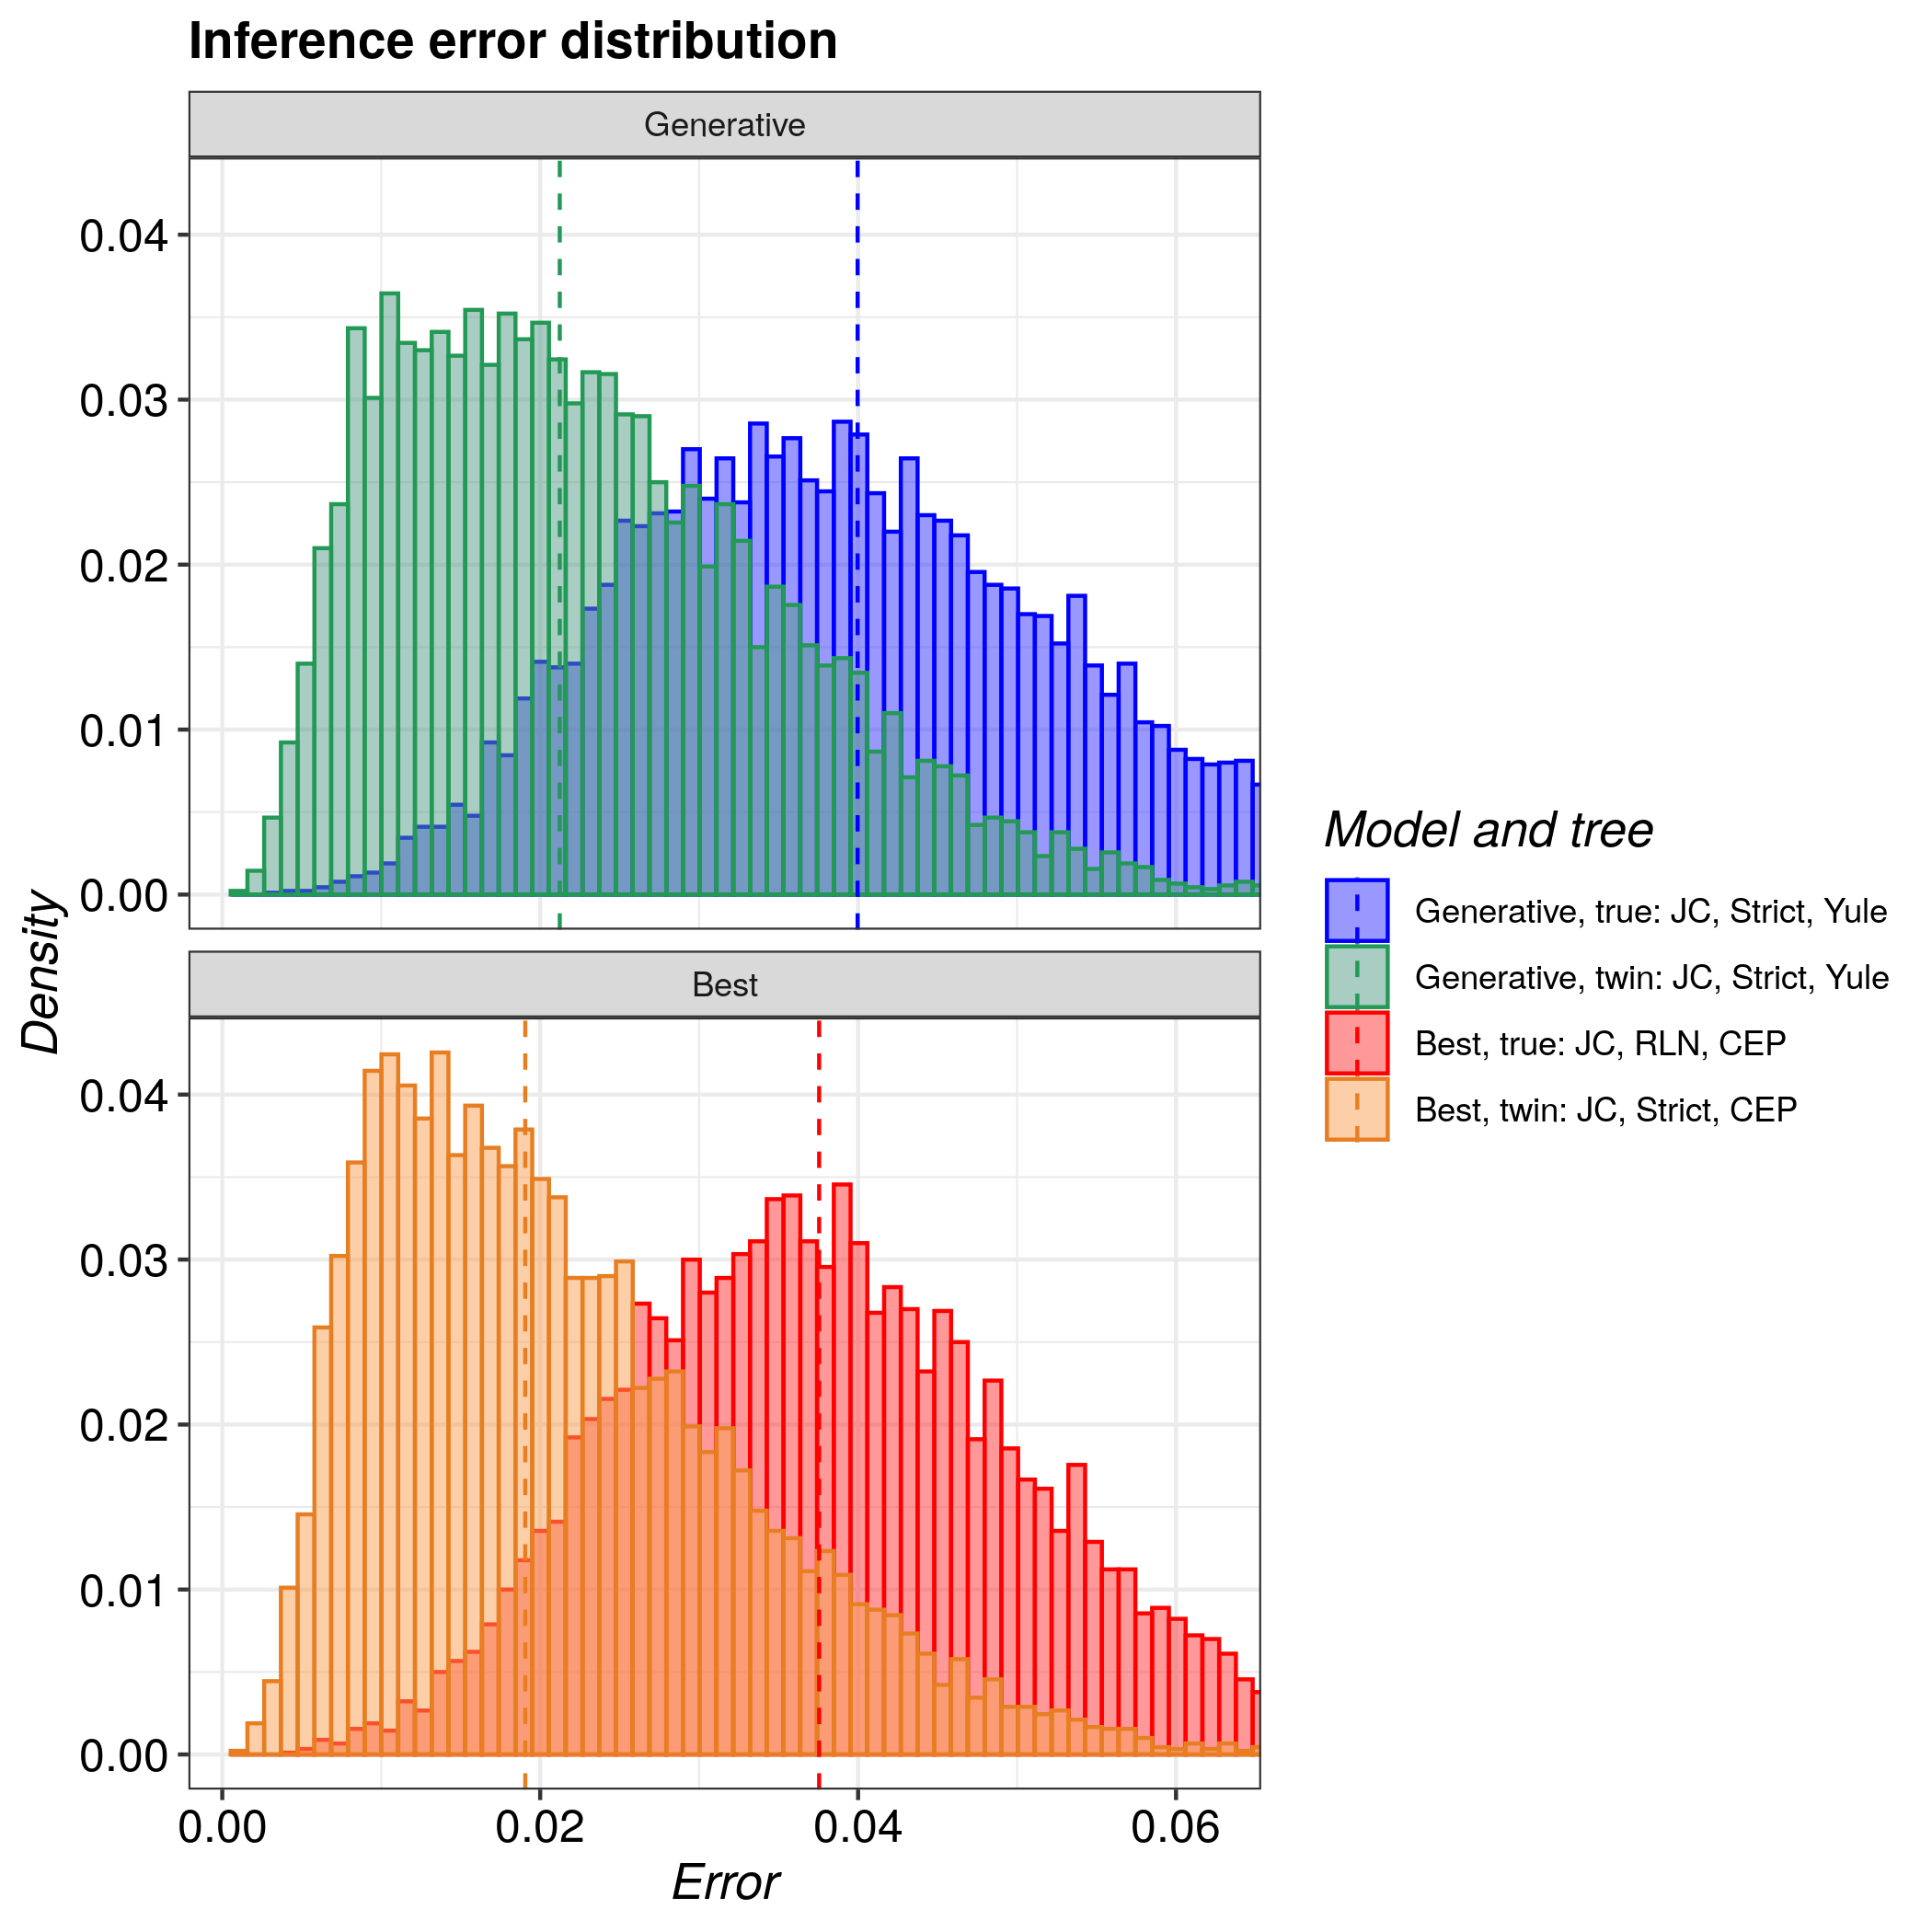
\includegraphics[width=\textwidth]{pirouette_example_3/example_3_314/errors.png}
  \caption{Equal number of mutations}
\end{figure}

\begin{figure}[H]
  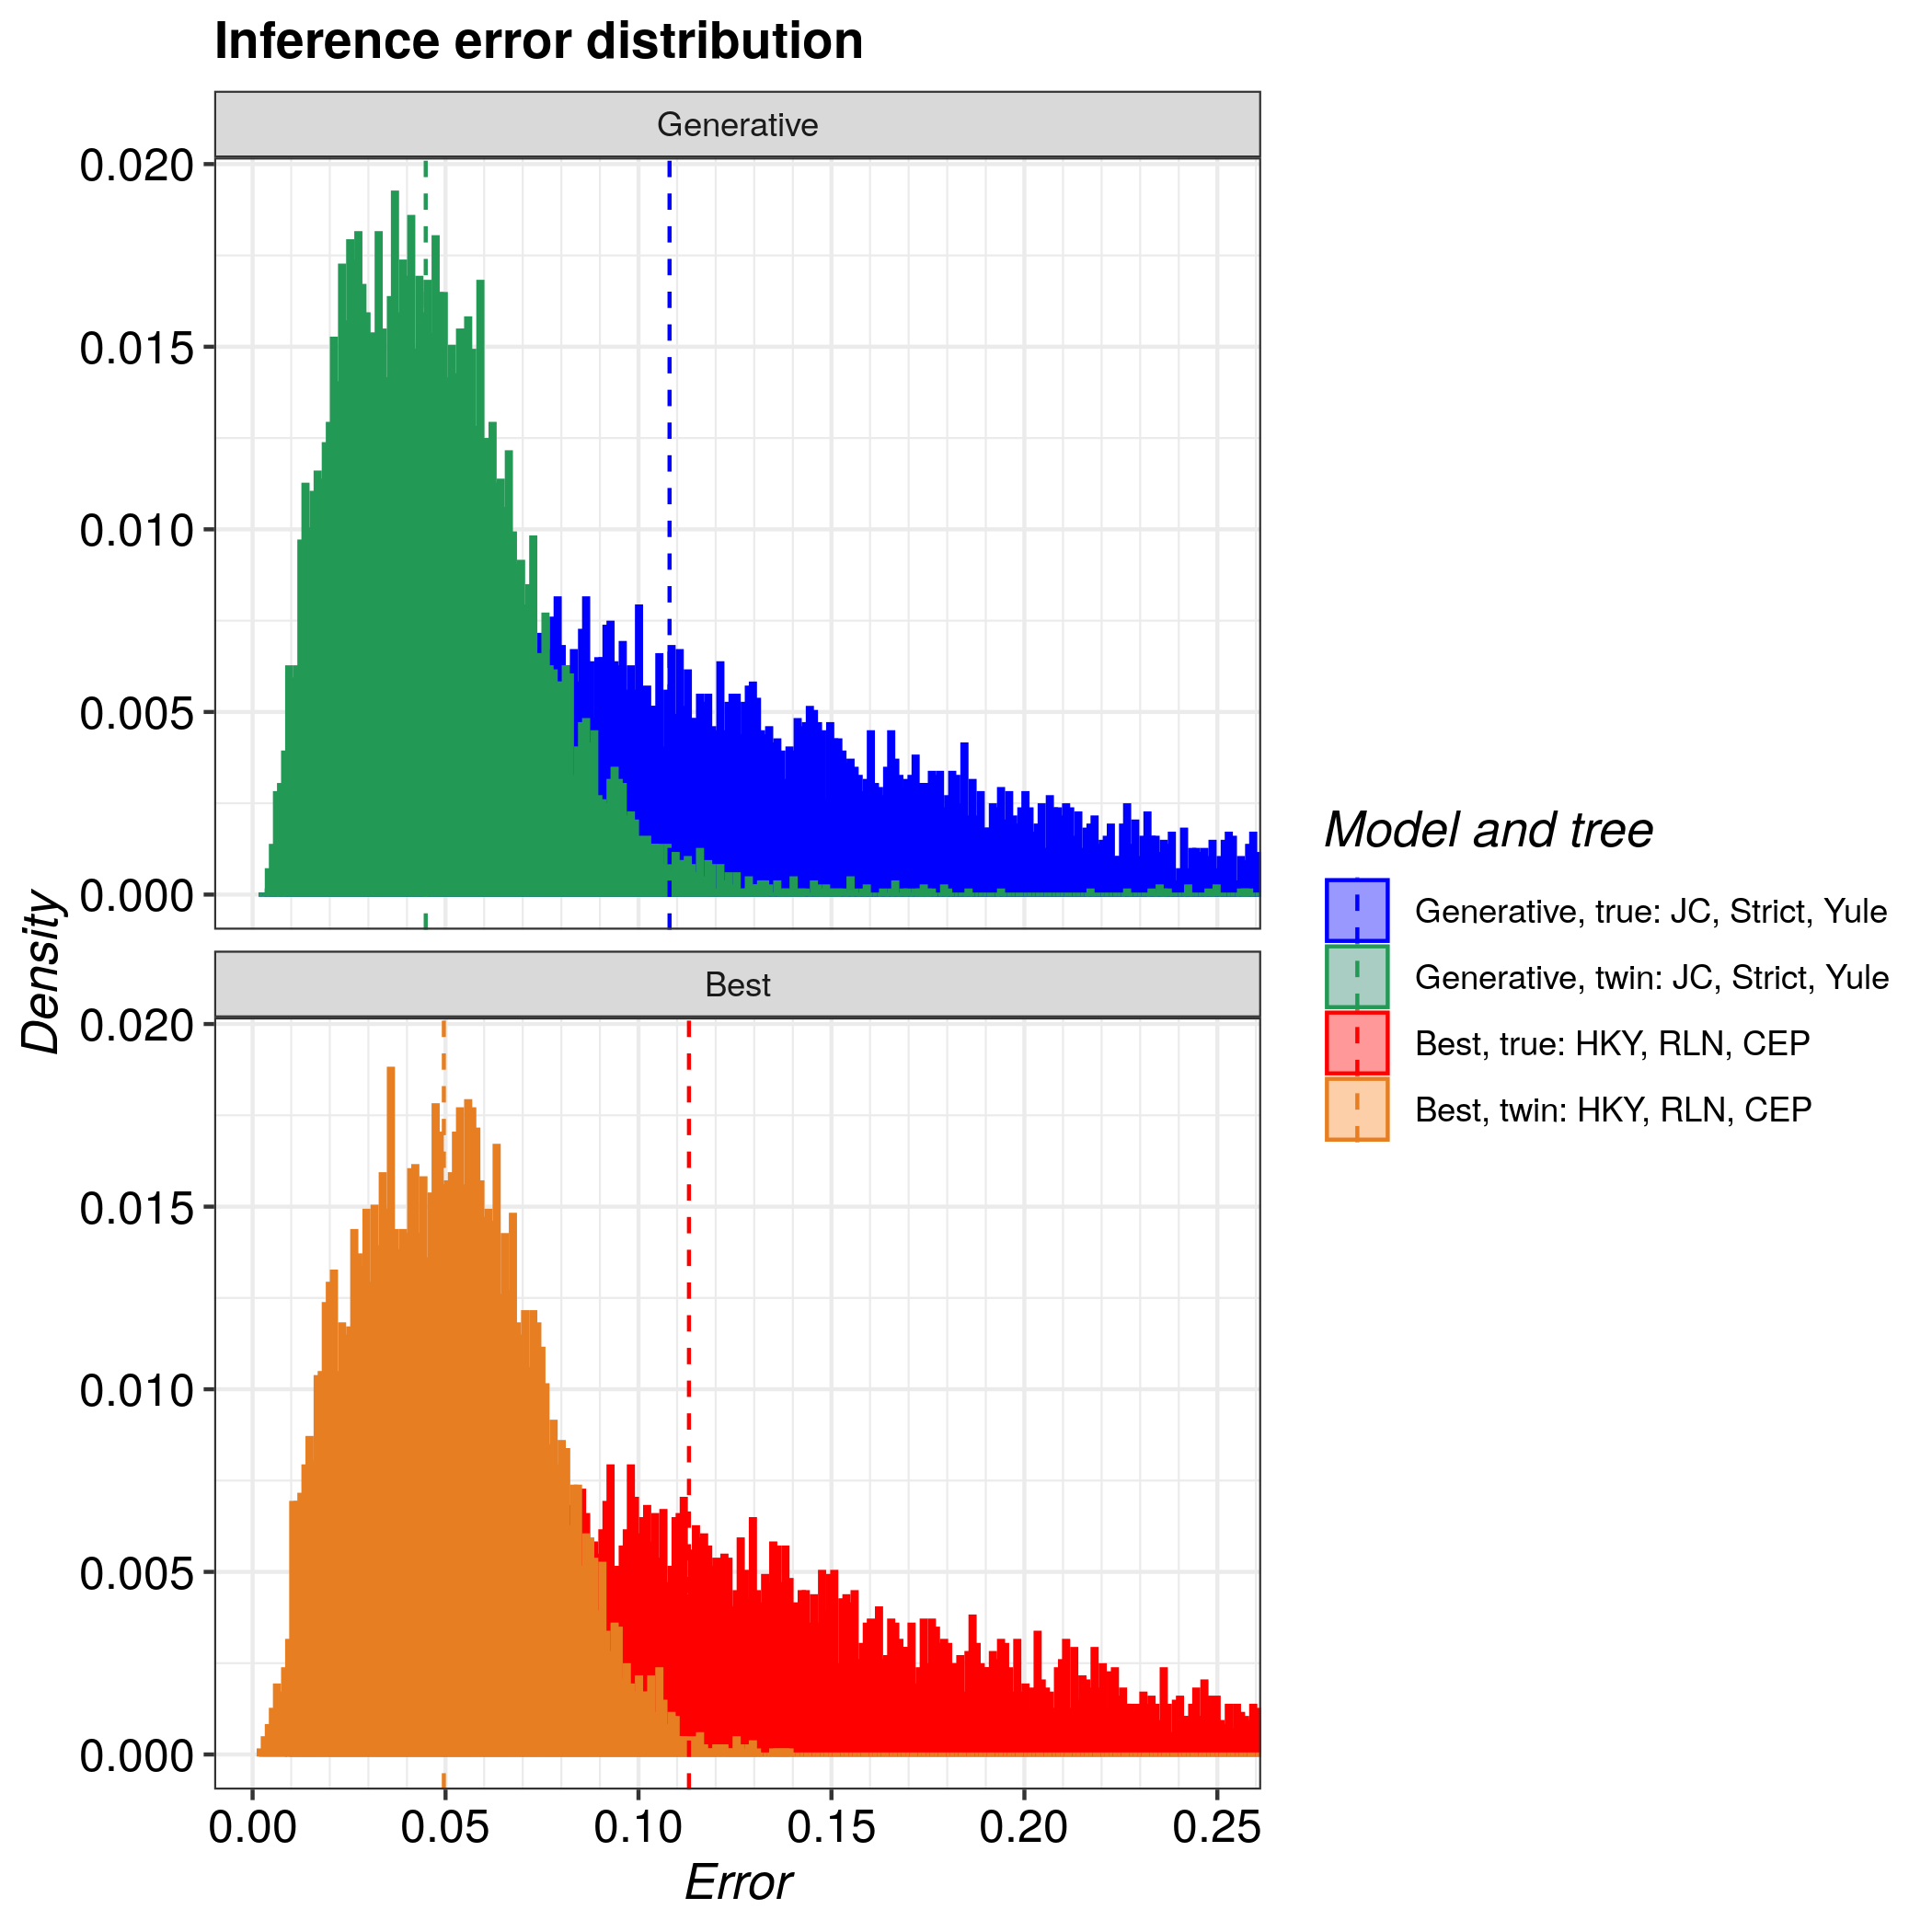
\includegraphics[width=\textwidth]{pirouette_example_18/example_18_314/errors.png}
  \caption{Equal mutation rate}
\end{figure}

%%%%%%%%%%%%%%%%%%%%%%%%%%%%%%%%%%%%%%%%%%%%%%%%%%%%%%%%%%%%%%%%%%%%%%%%%%%%%%%%
\subsection{The effect of mutation rate}
%%%%%%%%%%%%%%%%%%%%%%%%%%%%%%%%%%%%%%%%%%%%%%%%%%%%%%%%%%%%%%%%%%%%%%%%%%%%%%%%

The code used in this part of the article can be found at 
\url{https://github.com/richelbilderbeek/pirouette_example_24}.

\begin{figure}[H]
  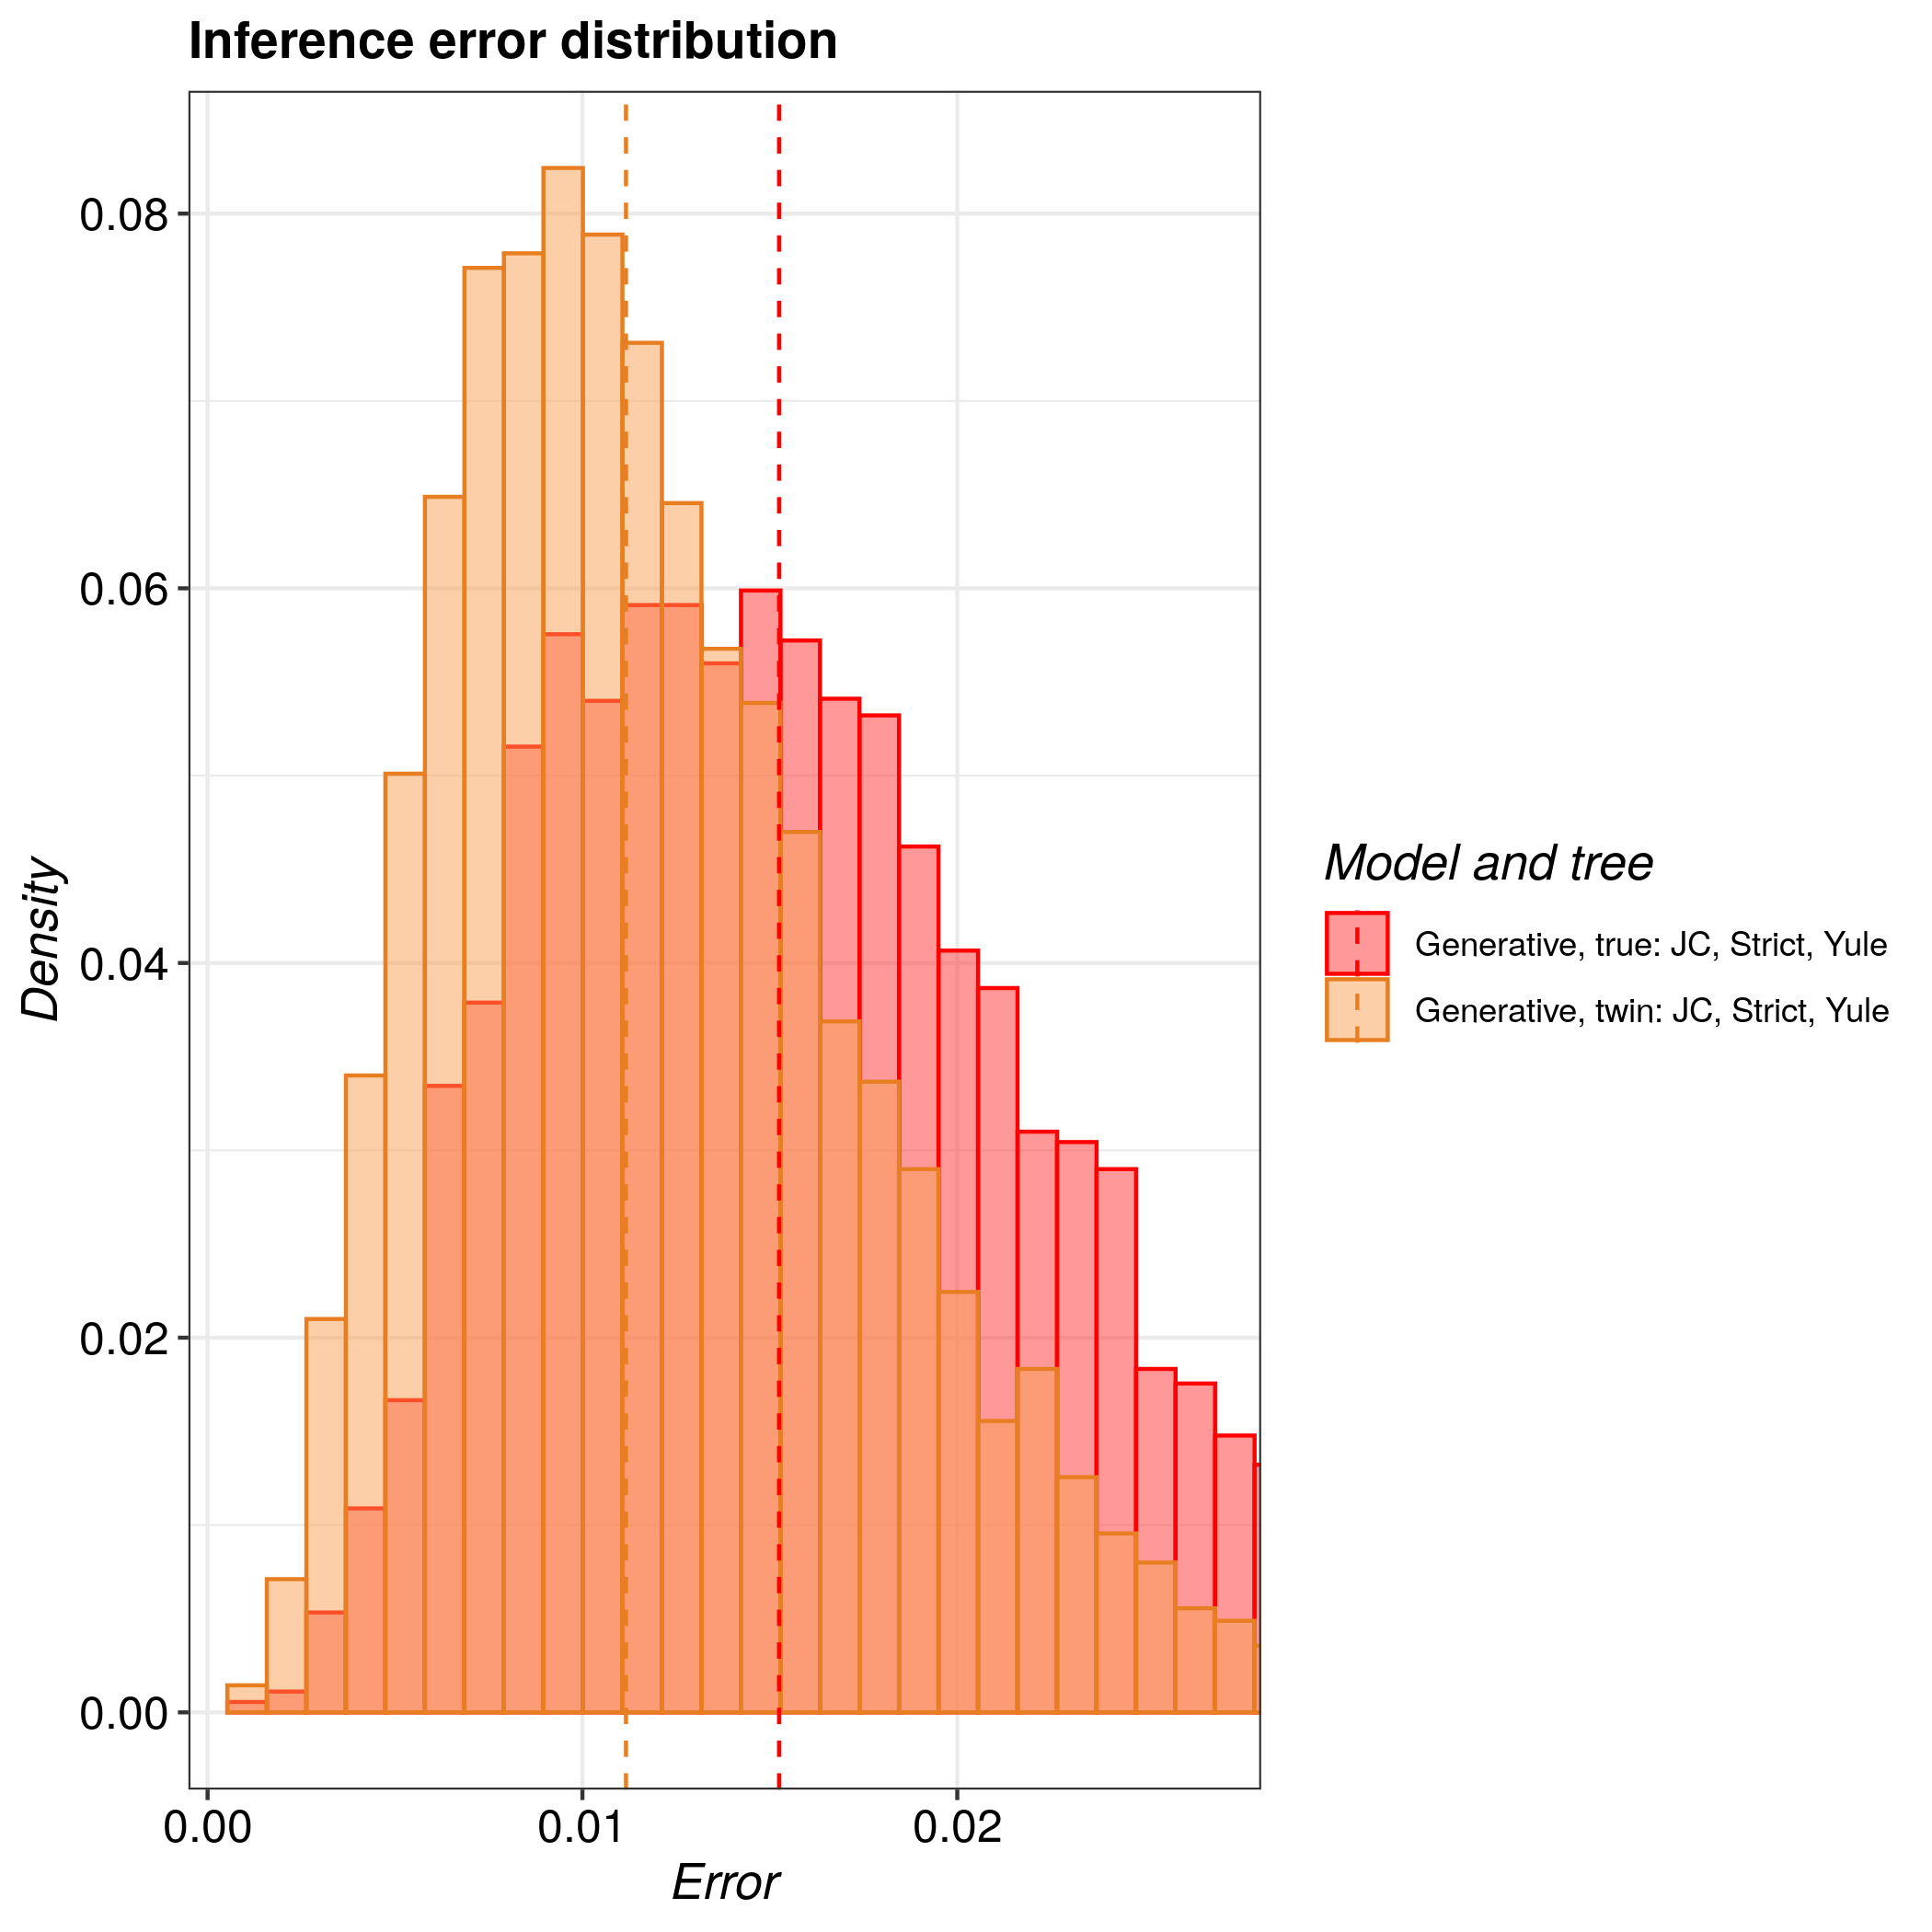
\includegraphics[width=\textwidth]{pirouette_example_24/example_24_314/errors.png}
  \caption{Per-nucleotide mutation rate of 0.0125}
\end{figure}


\begin{figure}[H]
  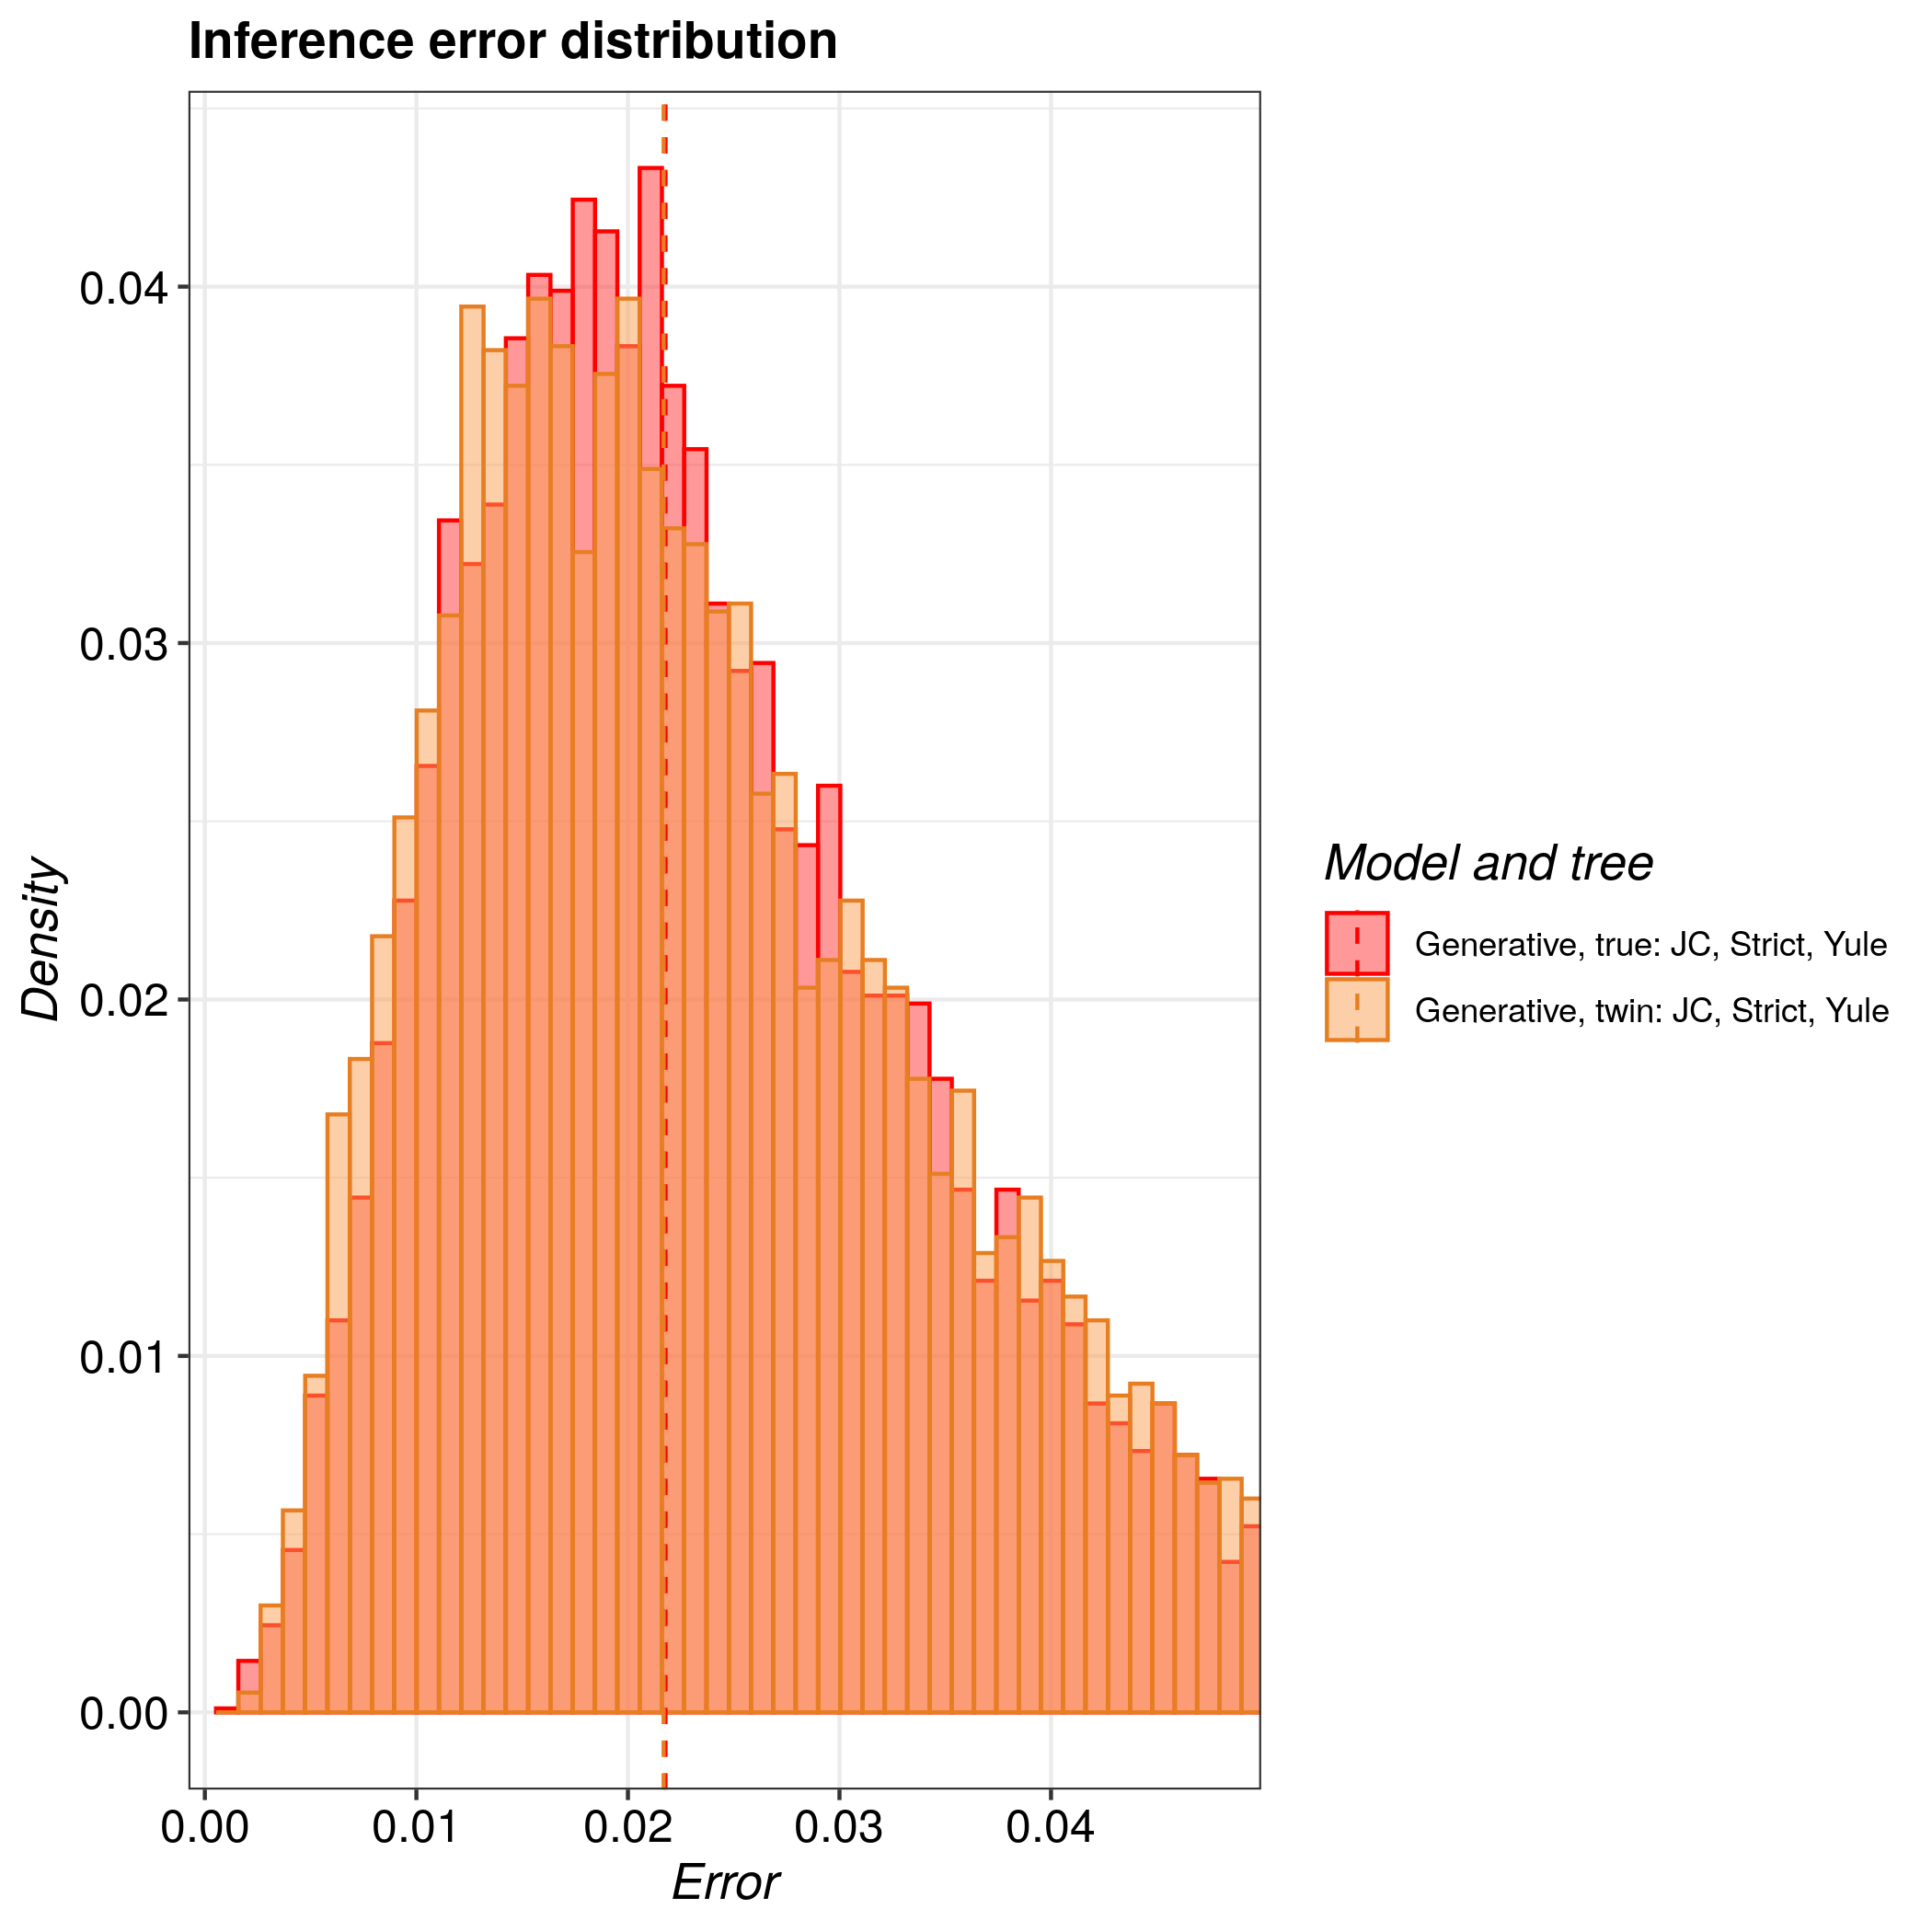
\includegraphics[width=\textwidth]{pirouette_example_24/example_24_315/errors.png}
  \caption{Per-nucleotide mutation rate of 0.025}
\end{figure}

\begin{figure}[H]
  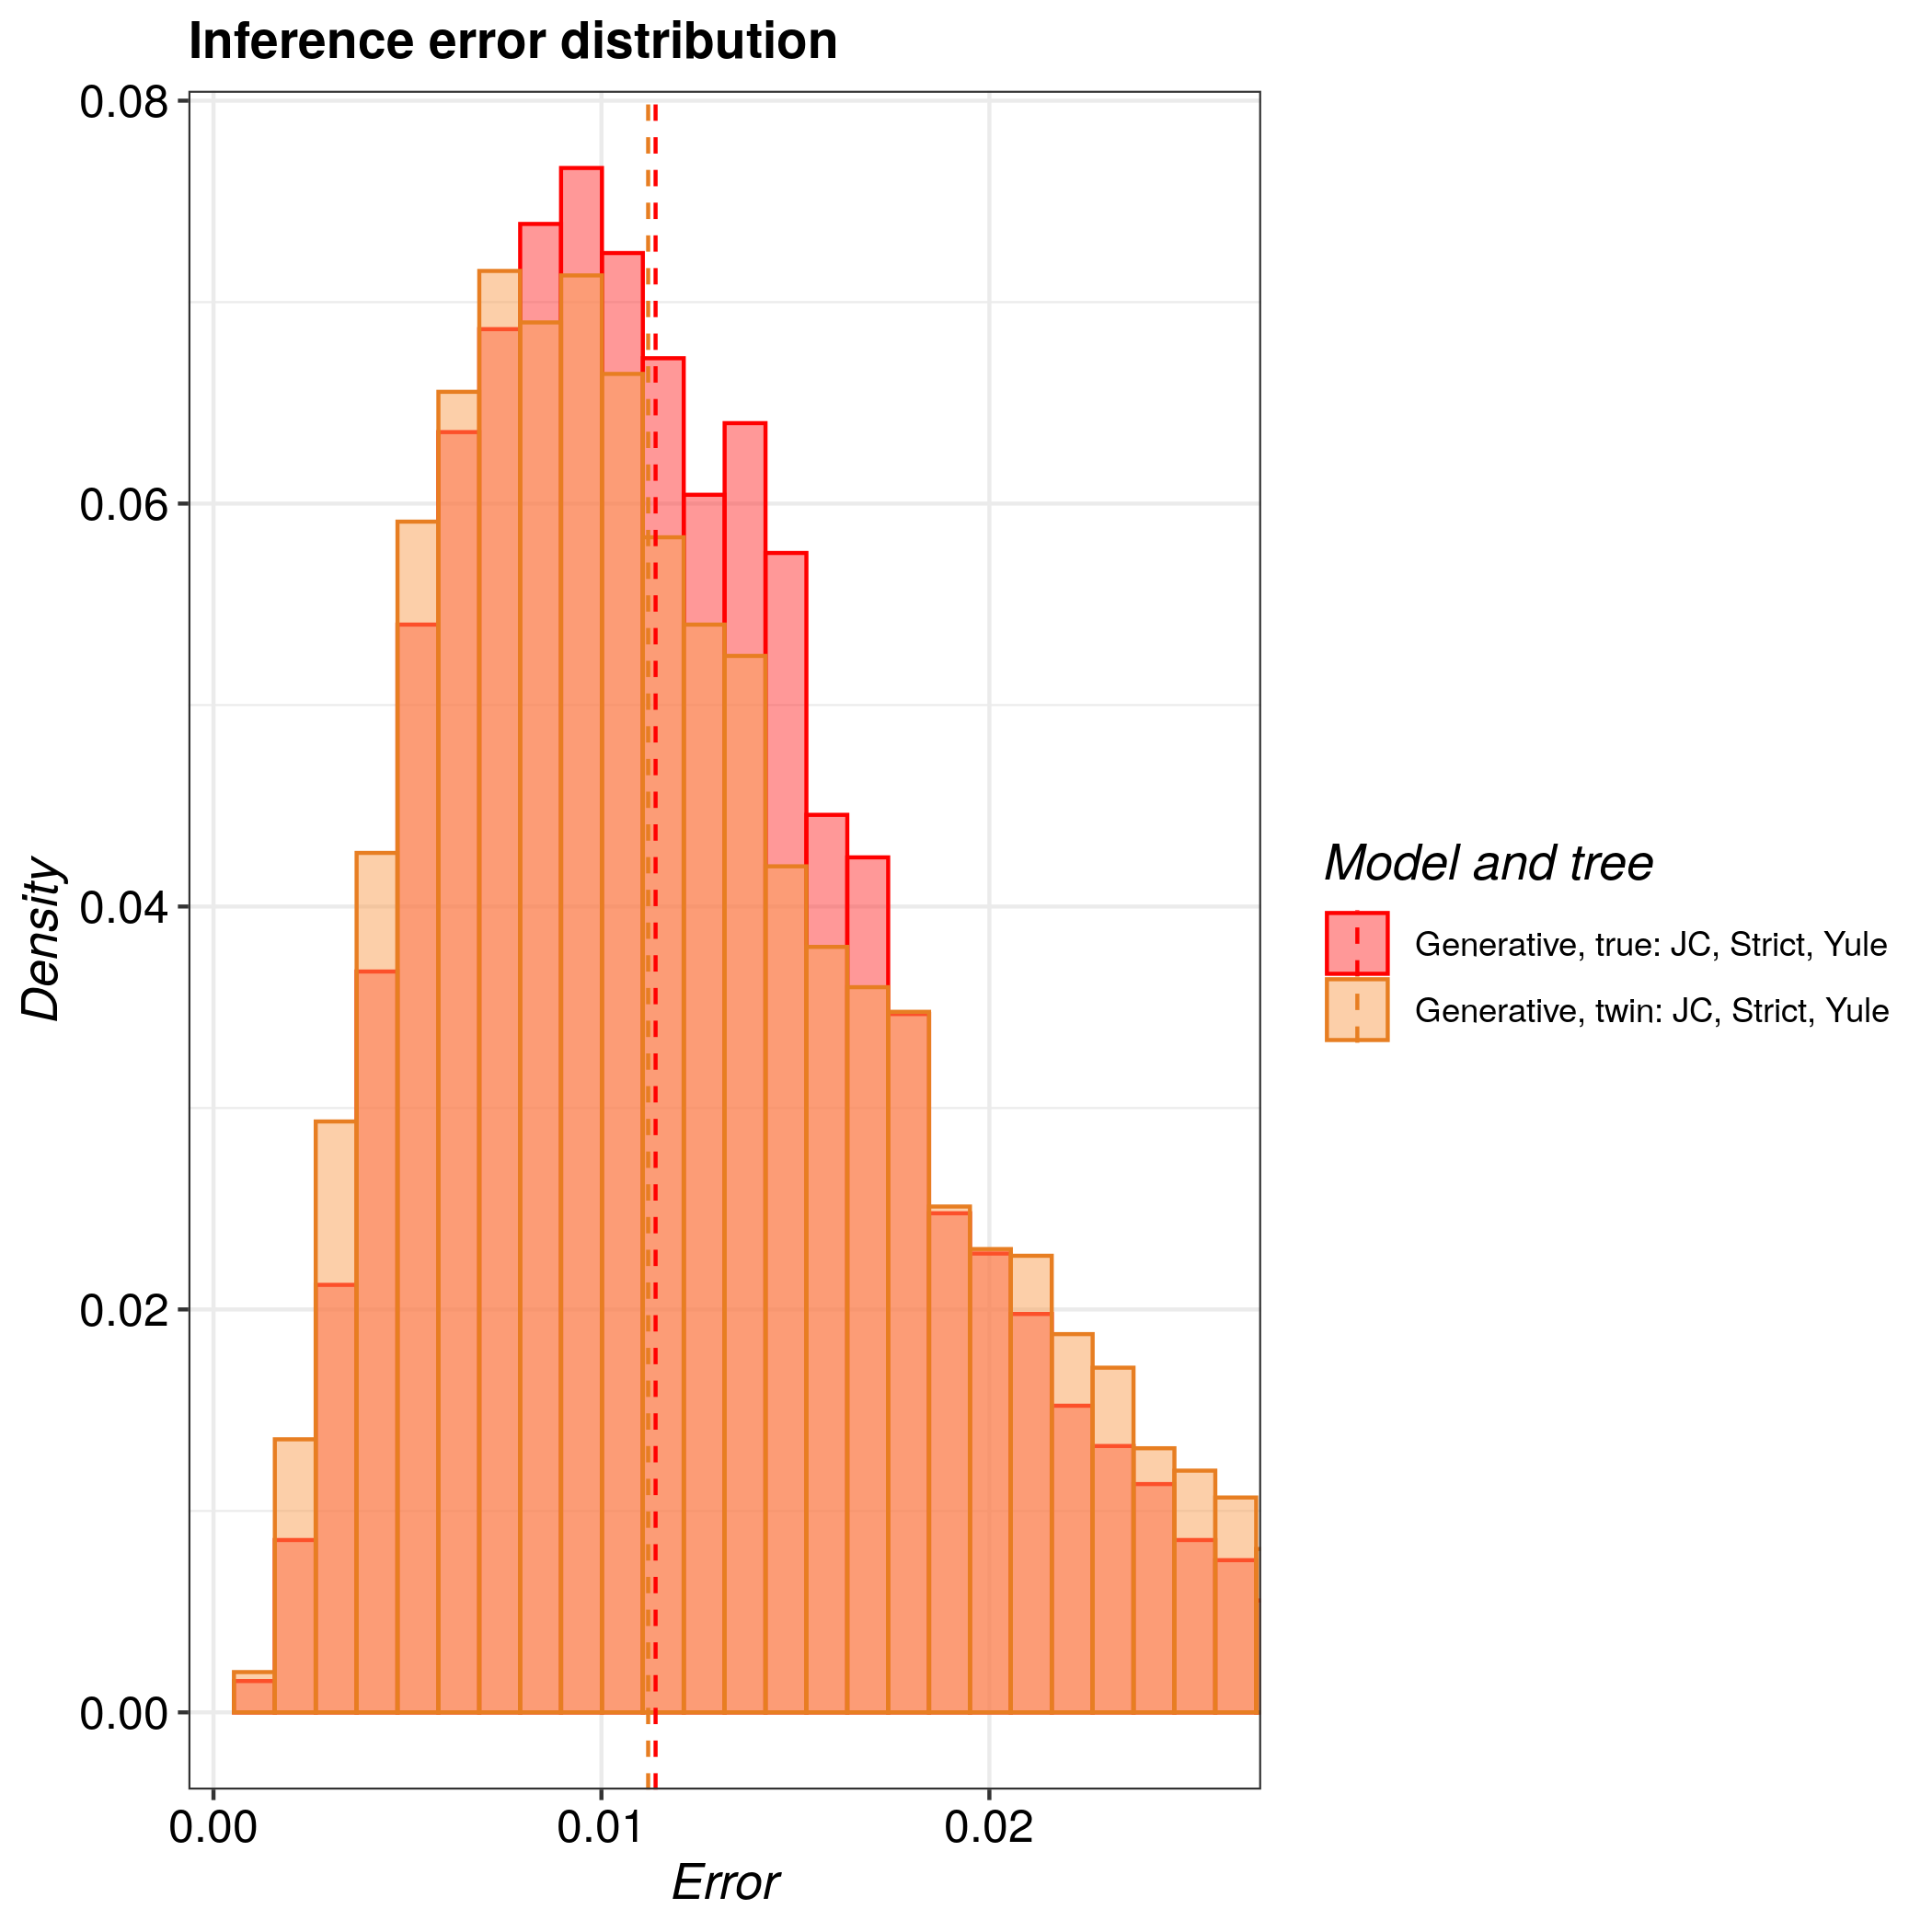
\includegraphics[width=\textwidth]{pirouette_example_24/example_24_316/errors.png}
  \caption{Per-nucleotide mutation rate of 0.05}
\end{figure}

\begin{figure}[H]
  \includegraphics[width=\textwidth]{pirouette_example_24/example_24_317/errors.png}
  \caption{Per-nucleotide mutation rate of 0.1}
\end{figure}

\begin{figure}[H]
  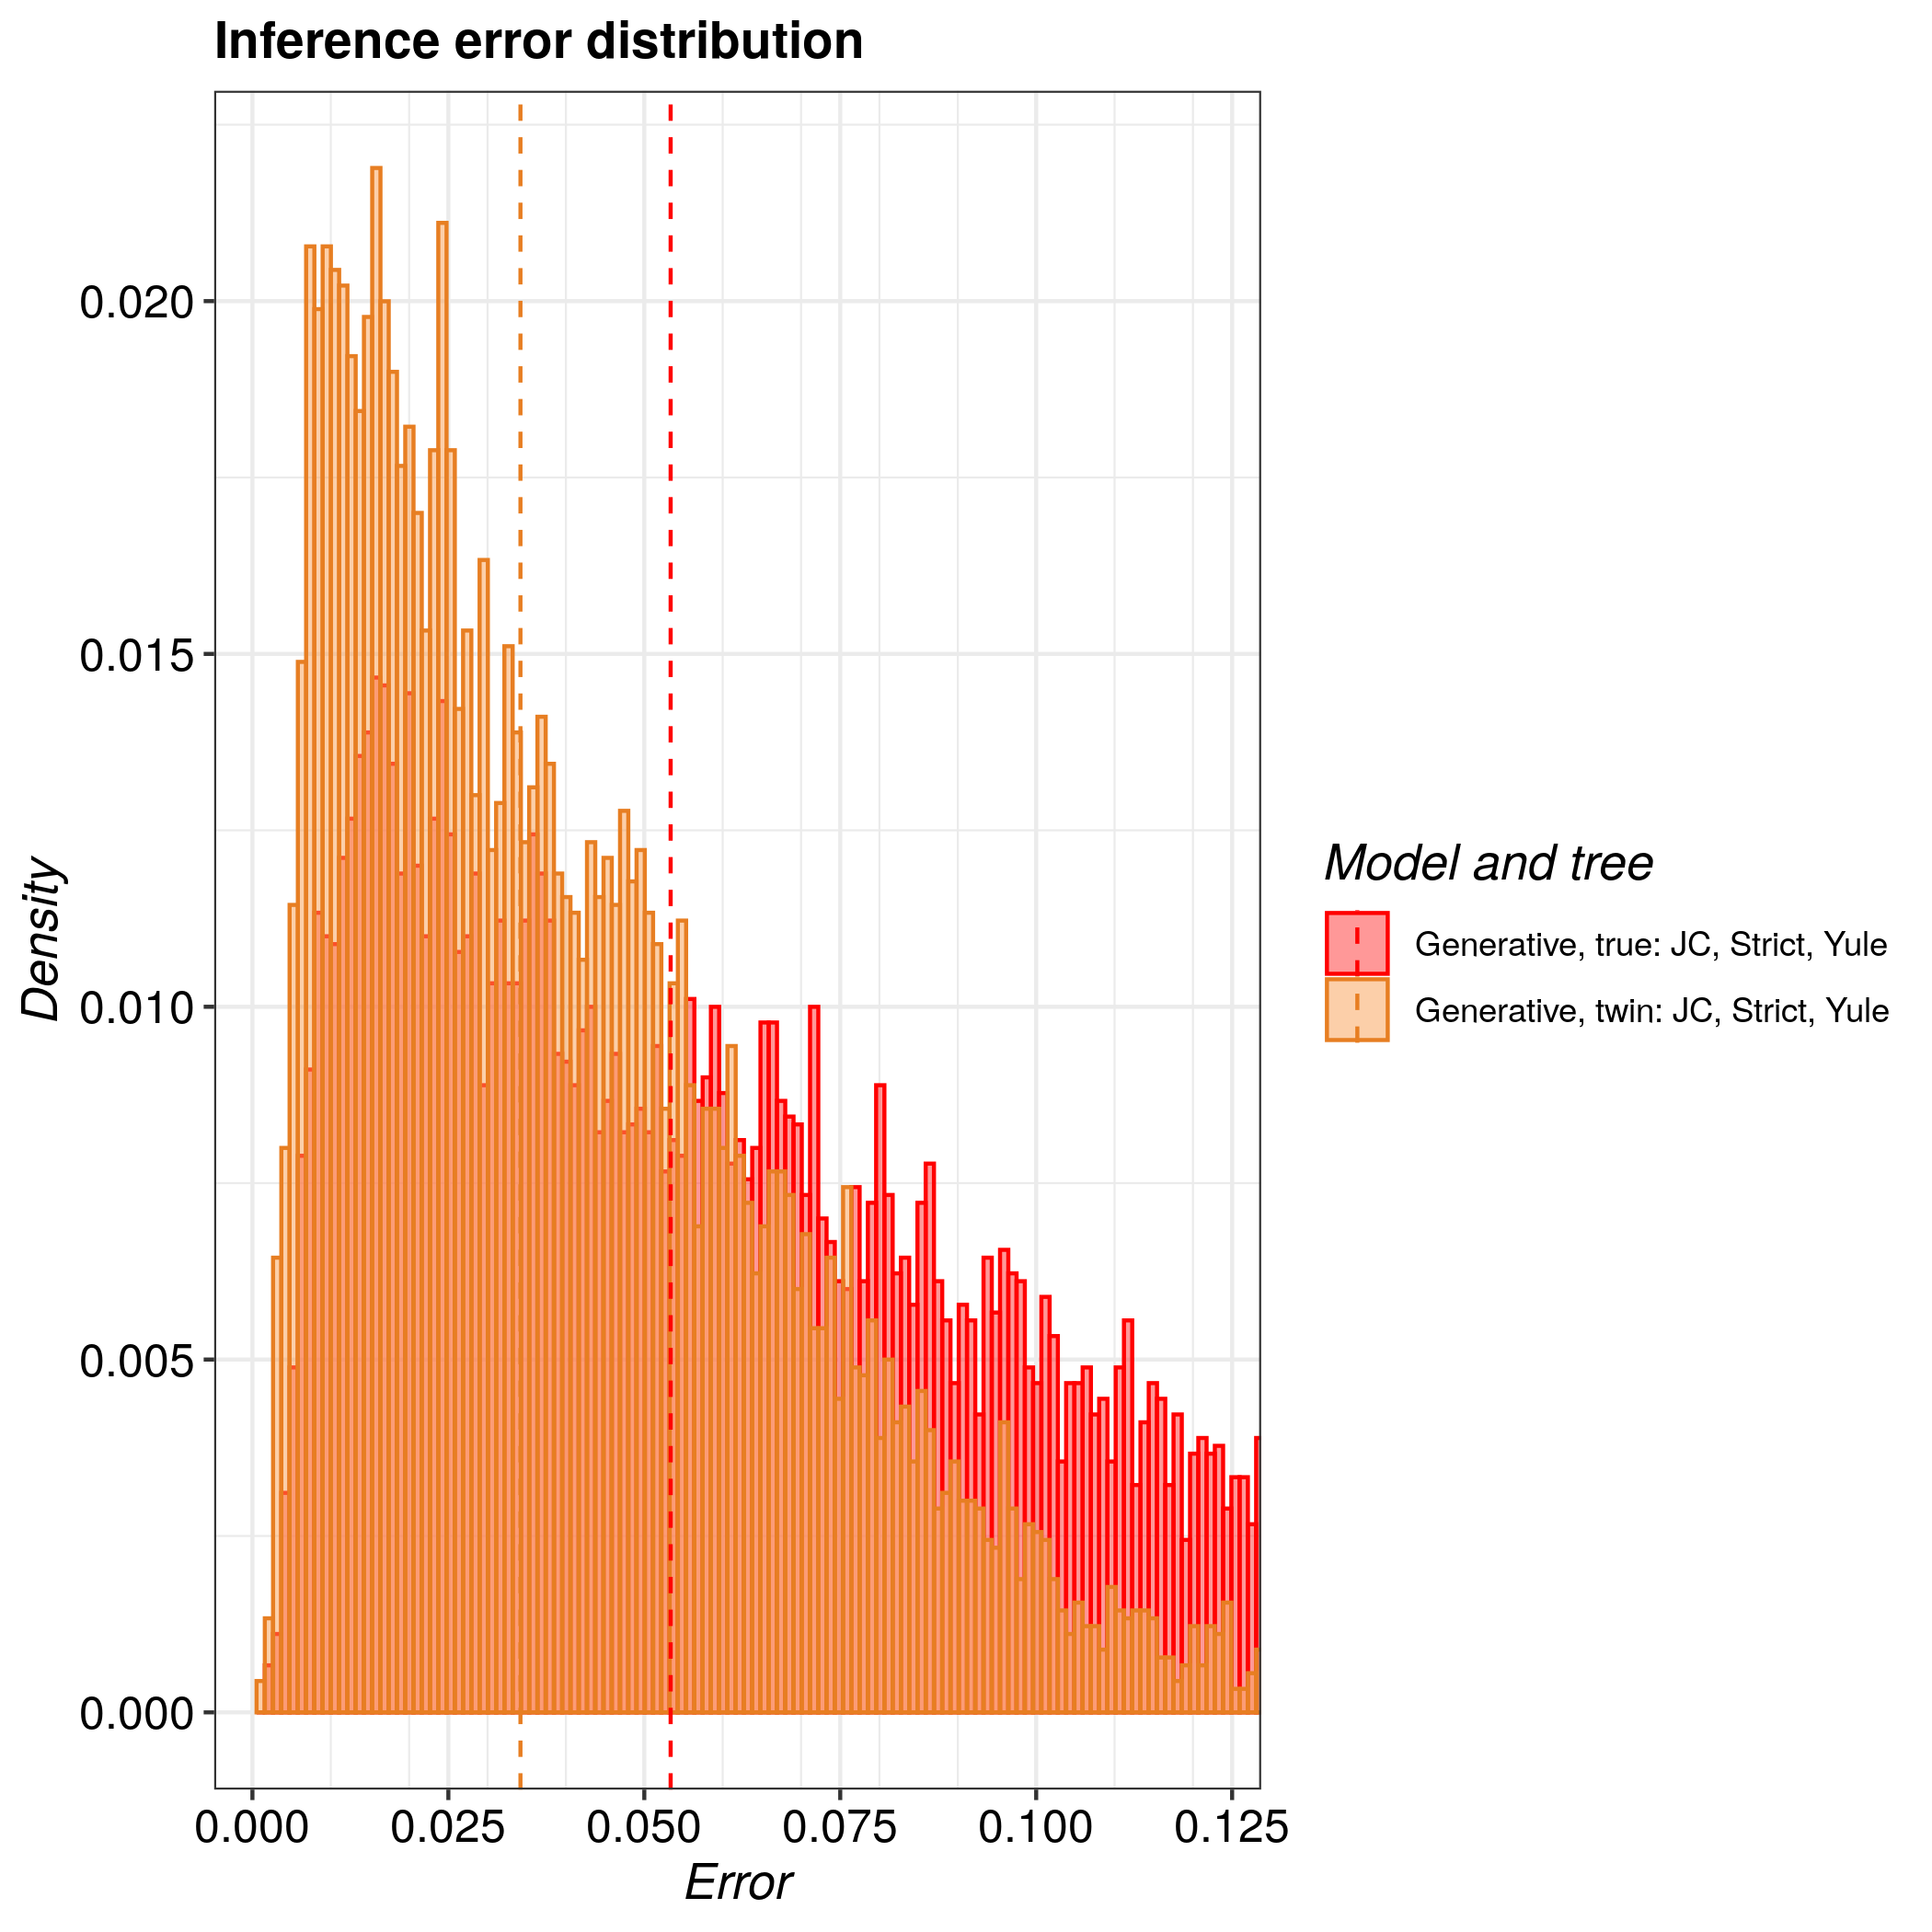
\includegraphics[width=\textwidth]{pirouette_example_24/example_24_318/errors.png}
  \caption{Per-nucleotide mutation rate of 0.2}
\end{figure}

\begin{figure}[H]
  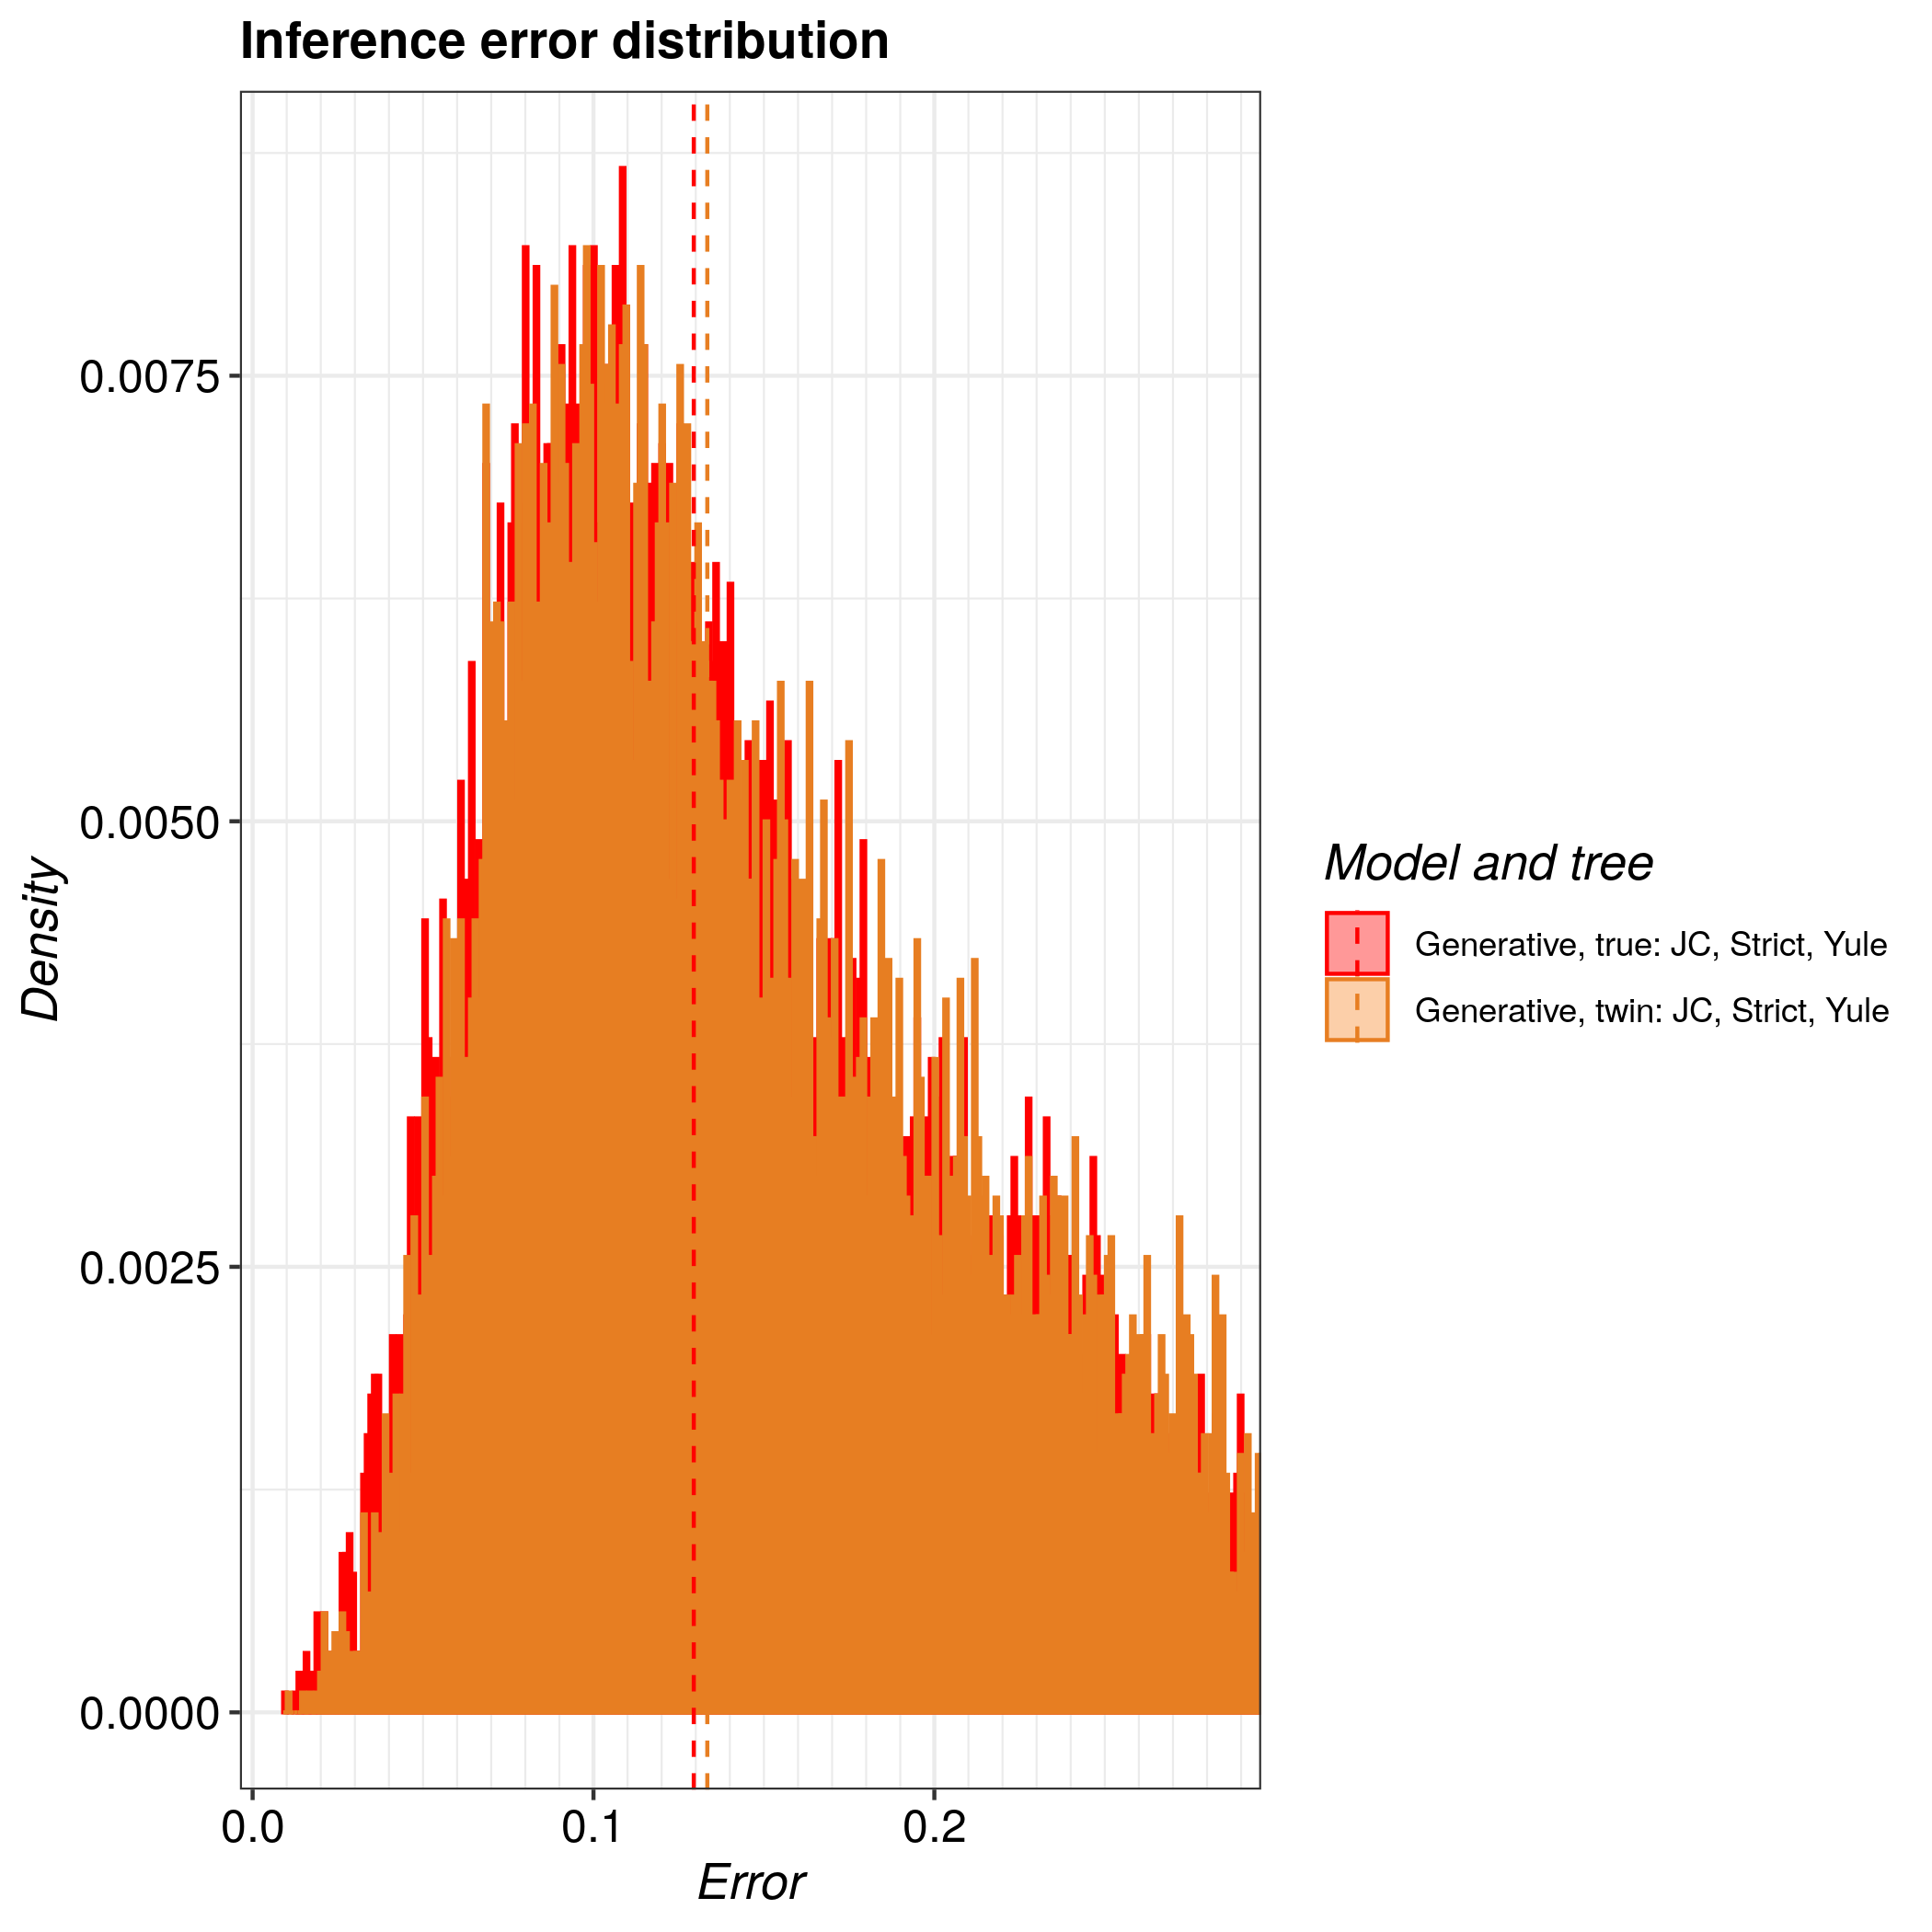
\includegraphics[width=\textwidth]{pirouette_example_24/example_24_319/errors.png}
  \caption{Per-nucleotide mutation rate of 0.4}
\end{figure}

\begin{figure}[H]
  \includegraphics[width=\textwidth]{pirouette_example_24/example_24_320/errors.png}
  \caption{Per-nucleotide mutation rate of 0.8}
\end{figure}

